%-------------------------------------------------------------------------------
% This file provides a skeleton ATLAS note.
% \pdfinclusioncopyfonts=1
% This command may be needed in order to get \ell in PDF plots to appear. Found in
% https://tex.stackexchange.com/questions/322010/pdflatex-glyph-undefined-symbols-disappear-from-included-pdf
%-------------------------------------------------------------------------------
% Specify where ATLAS LaTeX style files can be found.
\newcommand*{\ATLASLATEXPATH}{latex/}
% Use this variant if the files are in a central location, e.g. $HOME/texmf.
% \newcommand*{\ATLASLATEXPATH}{}
%-------------------------------------------------------------------------------
\documentclass[NOTE, atlasdraft=true, texlive=2016, UKenglish]{\ATLASLATEXPATH atlasdoc}
% The language of the document must be set: usually UKenglish or USenglish.
% british and american also work!
% Commonly used options:
%  atlasdraft=true|false This document is an ATLAS draft.
%  texlive=YYYY          Specify TeX Live version (2016 is default).
%  coverpage             Create ATLAS draft cover page for collaboration circulation.
%                        See atlas-draft-cover.tex for a list of variables that should be defined.
%  cernpreprint          Create front page for a CERN preprint.
%                        See atlas-preprint-cover.tex for a list of variables that should be defined.
%  NOTE                  The document is an ATLAS note (draft).
%  PAPER                 The document is an ATLAS paper (draft).
%  CONF                  The document is a CONF note (draft).
%  PUB                   The document is a PUB note (draft).
%  BOOK                  The document is of book form, like an LOI or TDR (draft)
%  txfonts=true|false    Use txfonts rather than the default newtx
%  paper=a4|letter       Set paper size to A4 (default) or letter.

%-------------------------------------------------------------------------------
% Extra packages:
\usepackage{\ATLASLATEXPATH atlaspackage}
% Commonly used options:
%  biblatex=true|false   Use biblatex (default) or bibtex for the bibliography.
%  backend=bibtex        Use the bibtex backend rather than biber.
%  subfigure|subfig|subcaption  to use one of these packages for figures in figures.
%  minimal               Minimal set of packages.
%  default               Standard set of packages.
%  full                  Full set of packages.
%-------------------------------------------------------------------------------
% Style file with biblatex options for ATLAS documents.
\usepackage{\ATLASLATEXPATH atlasbiblatex}

% Package for creating list of authors and contributors to the analysis.
\usepackage{\ATLASLATEXPATH atlascontribute}

% Useful macros
\usepackage{\ATLASLATEXPATH atlasphysics}
% See doc/atlas_physics.pdf for a list of the defined symbols.
% Default options are:
%   true:  journal, misc, particle, unit, xref
%   false: BSM, heppparticle, hepprocess, hion, jetetmiss, math, process, other, texmf
% See the package for details on the options.

% Files with references for use with biblatex.
% Note that biber gives an error if it finds empty bib files.
\addbibresource{ANA-STDM-2018-50-INT1.bib}
\addbibresource{bib/ATLAS.bib}
\addbibresource{bib/CMS.bib}
\addbibresource{bib/ConfNotes.bib}
\addbibresource{bib/PubNotes.bib}

% Paths for figures - do not forget the / at the end of the directory name.
\graphicspath{{logos/}{figures/}}

% Add you own definitions here (file ANA-STDM-2018-50-INT1-defs.sty).
\usepackage{ANA-STDM-2018-50-INT1-defs}

%-------------------------------------------------------------------------------
% Generic document information
%-------------------------------------------------------------------------------

% Title, abstract and document
%-------------------------------------------------------------------------------
% This file contains the title, author and abstract.
% It also contains all relevant document numbers used for an ATLAS note.
%-------------------------------------------------------------------------------

% Title
\AtlasTitle{ Lepton (non)-universality in W decays in Run 2 with low mu data}

% Draft version:
% Should be 1.0 for the first circulation, and 2.0 for the second circulation.
% If given, adds draft version on front page, a 'DRAFT' box on top of each other page, 
% and line numbers.
% Comment or remove in final version.
\AtlasVersion{0.1}

% Abstract - % directly after { is important for correct indentation
\AtlasAbstract{%
  Interesting hints of lepton non-universality have been seen in decays of B hadrons.  
  Measurements from LEP on W decays also show a hint of non universality at the level of a few percent. 
  The ATLAS experiment has produced over $10^9$ W decays to leptons, which allows us to make a high-precision measurement of lepton (non)-universality in W decay by measuring the ratio $R_{\tau/\mu} =  BR (W\rightarrow \tau\nu \rightarrow \mu\nu\bar{\nu}) / BR (W \rightarrow \mu\nu)$, in which many systematic effects are cancel. 
  Main challenges are control of the non-W background and trigger related systematics.
  Our results \todo{agree/disagree} with the value of $R_{\tau/\mu} = 1$ expected in the case of Lepton Flavour Universality as predicted by the Standard Model.
}

% Author - this does not work with revtex (add it after \begin{document})
% \author{The ATLAS Collaboration}

% Authors and list of contributors to the analysis
% \AtlasAuthorContributor also adds the name to the author list
% Include package latex/atlascontribute to use this
% Use authblk package if there are multiple authors, which is included by latex/atlascontribute
% \usepackage{authblk}
% Use the following 3 lines to have all institutes on one line
% \makeatletter
% \renewcommand\AB@affilsepx{, \protect\Affilfont}
% \makeatother
% \renewcommand\Authands{, } % avoid ``. and'' for last author
% \renewcommand\Affilfont{\itshape\small} % affiliation formatting
% \AtlasAuthorContributor{First AtlasAuthorContributor}{a}{Author's contribution.}
% \AtlasAuthorContributor{Second AtlasAuthorContributor}{b}{Author's contribution.}
% \AtlasAuthorContributor{Third AtlasAuthorContributor}{a}{Author's contribution.}
% \AtlasContributor{Fourth AtlasContributor}{Contribution to the analysis.}
% \author[a]{First Author}
% \author[a]{Second Author}
% \author[b]{Third Author}
% \affil[a]{One Institution}
% \affil[b]{Another Institution}

\AtlasAuthorContributor{Daniil Ponomarenko}{a, b}{Software development. Data/MC studies and selection optimisation. Fake background estimation and Z control region studies. Control plots, preliminary fit and preliminary systematics.}
\AtlasAuthorContributor{Jia Jia Teoh}{a}{ Corrections and calibrations for d0. Studies for Ztt region.}
\AtlasAuthorContributor{Nataliia Zakharchuk}{c}{ Software development advisor. Z cross checks. Supporting note.}
\AtlasAuthorContributor{Nicolo de Groot}{a}{General analysis supervision.}
\affil[a]{Radboud University}
\affil[b]{Moscow MEPhI}
\affil[c]{Carleton University}


% If a special author list should be indicated via a link use the following code:
% Include the two lines below if you do not use atlasstyle:
% \usepackage[marginal,hang]{footmisc}
% \setlength{\footnotemargin}{0.5em}
% Use the following lines in all cases:
% \usepackage{authblk}
% \author{The ATLAS Collaboration%
% \thanks{The full author list can be found at:\newline
%   \url{https://atlas.web.cern.ch/Atlas/PUBNOTES/ATL-PHYS-PUB-2016-007/authorlist.pdf}}
% }

% ATLAS reference code, to help ATLAS members to locate the paper
\AtlasRefCode{ANA-STDM-2020-XX}

% ATLAS note number. Can be an COM, INT, PUB or CONF note
\AtlasNote{ANA-STDM-2020-XX-INTX}

% Author and title for the PDF file
\hypersetup{pdftitle={ATLAS document},pdfauthor={The ATLAS Collaboration}}

%-------------------------------------------------------------------------------
% Content
%-------------------------------------------------------------------------------
\begin{document}

\maketitle

\tableofcontents

% List of contributors - print here or after the Bibliography.
%\PrintAtlasContribute{0.30}

\clearpage
%-------------------------------------------------------------------------------
\section*{Preface}
\label{sec:preface}
%-------------------------------------------------------------------------------


\subsection*{Summary on major updates}

\begin{itemize}
\item \textbf{v0.1} First draft.

\item

\end{itemize}

\subsection*{To do list}


\clearpage
%-------------------------------------------------------------------------------
\section{Introduction}
\label{sec:intro}
%-------------------------------------------------------------------------------

Lepton universality is one of the cornerstones of the Standard Model of particle physics. 
In the past years interesting hints of lepton non-universality have been seen in semi-leptonic decays of B hadrons~\cite{HFLAV16} where an excess of $\tau$ final states over $e,\mu$ final states is seen at the level of 4 standard deviations.
Measurements from LEP on W decays also show a hint of non universality at the level of a few percent~\cite{LEP-2}, again with a surplus of $\tau$ final states: 
\begin{equation}
  \label{eq:LEP_BRoverBRAll}
  \frac{2BR(W\to\tau\nu)}{BR(W\to\mu\nu)+BR(W\to e\nu)} = 1.077 \pm 0.026
\end{equation}
resulting in a poor agreement at the level of 2.8 standard deviations, with all correlations included.

Both results are shown in Figure~\ref{fig:lnuhints}.

\begin{figure}[htbp]
\centering
\includegraphics[width=10cm]{figures/01_intro/rdrds_summer18.png}
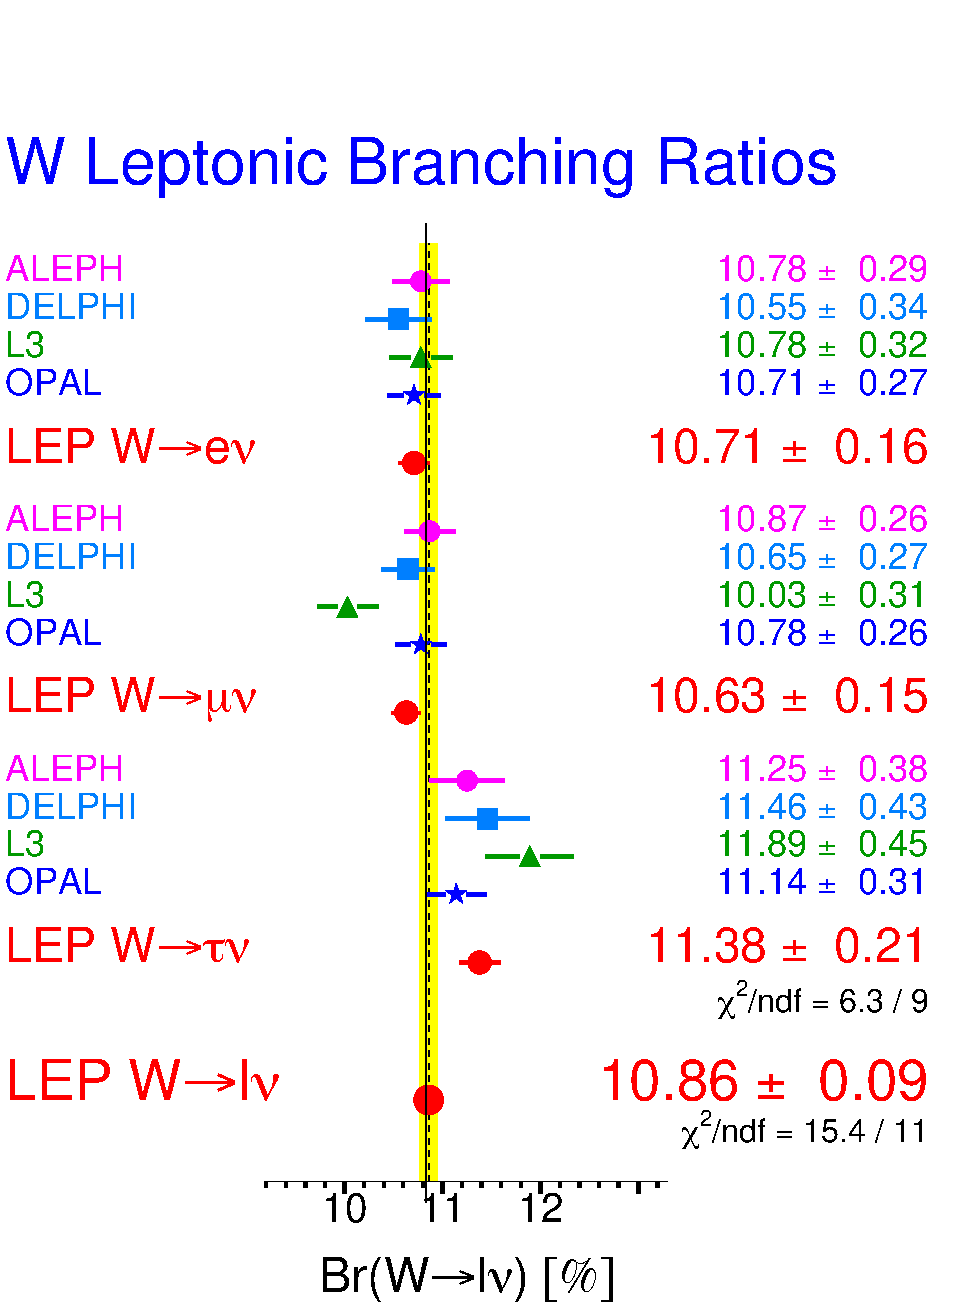
\includegraphics[width=6cm]{figures/01_intro/4f_brlv_lep_2008.pdf}
\caption{Left: Lepton universality in $B\to D^{(*)}$ decay from \cite{HFLAV16}. 
Right:  W leptonic branching ratios from \cite{LEP-2}}
\label{fig:lnuhints}
\end{figure}


\subsection{Summary of the Analysis Strategy}

The ATLAS experiment has produced over $10^9$ W decays to leptons, which allows us to make a high-precision measurement of lepton (non)-universality in prompt W decay by measuring the ratio $R_{\tau/\mu} =  BR (W\to \tau\nu \to \ell\nu\bar{\nu}) / BR (W \to \ell\nu)$, where $\ell = e, \mu$,  in which many of the systematic effects related to lepton identification cancel. 
Most leptons comes from prompt $W$ decay since the branching fraction of $\tau$ to leptons is 17.39 \% and many leptons coming from $W\to\tau\to \ell$ decay do not make it through the L1 trigger because of their lower momentum. 
Our first step is identification of the parts of the phase space enriched in $\tau$ decays using a multivariate classifier based on kinematic information and on the impact parameter of the lepton $d_0$.
Since these two variables are largely uncorrelated we can constrain the efficiency from data.

Same way as it is described in Top group analysis paper \cite{Mcfayden:2667199}, this analysis is setup to measure the ratio of the parameter of interest $R(\tau/\mu)$ in data and MC:
\begin{equation}
  \label{eq:fit_poi}
  \mu_{R(\tau/\mu)} = R^{full}(\tau/\mu) = \frac{BR(W\to\tau\nu)}{BR(W\to\mu\nu)}
\end{equation}
But instead of measuring tag and prompt leptons, we are working with single lepton triggers. 
This leads us to one of the main analysis challenges: good control over single trigger related systematics.


Control regions are defined to constrain the modelling of the major backgrounds: $Z\to\ell\ell$ boson production and QCD fake leptons.
Additional $Z\to\tau\tau$ leptonic control region is get used for $d_0$ correction studies.

Similarly as it was done in \cite{Mcfayden:2667199}, we define next list of categories of leptons according to their truth origin:
\begin{itemize}
\item \textbf{prompt ($W$)} leptons are leptons produced in $W\to\ell\nu$ decays.
\item \textbf{tau} are leptons produced in the leptonic decay chain $W \to \tau\nu \to \ell\nu\bar{\nu}$.
\item \textbf{prompt (non-$W$)} are leptons from $Z^0$ or other EWK process where these leptons do not originate from $W$ decays: for example di-boson, single top or $t\bar{t}$ process.
\item \textbf{``fake''} are reconstructed leptons from all other sources, including wrongly identified leptons.
\end{itemize}

A two-dimensional fit is performed in BDT and $d_0$ of the lepton.
The overall rate of the $W$ events is allowed to float along with the property of interest -- the ratio of $W \to \tau\nu$ to $W \to \ell\nu$ events.
The combined $d_0$--$p_T$ fit allows the best separation between prompt-, tau- and fake leptons.

Initial studies are performed for both electron and muon $W$ decay channels, but we focus on the ratio to muons rather then electrons for this analysis due to the lower rate of bremsstrahlung of muons and lower fakes background contribution.


% %-------------------------------------------------------------------------------
% \section{Data and MC Samples}
% \label{sec:data_and_mc_samples}
% %-------------------------------------------------------------------------------
% 
The analysis is performed on the low pile-up data samples of pp collisions at $\sqrt{s}=13$~TeV collected by ATLAS in 2017 and 2018 years.

Event selection is the same as used for low pile-up analysis paper~\cite{Kretzschmar:2657141}.

The full list is given in Appendix~\ref{sec:details_on_list_of_MC_samples}.








% %-------------------------------------------------------------------------------
% \section{Object Identification}
% \label{sec:object_identification}
% %-------------------------------------------------------------------------------
% % https://glance.cern.ch/atlas/analysis/analyses/details?id=1186

Same as for low pile-up analysis. 
Muon corrections~\cite{Sydorenko:2657116}.
Hadronic recoil reconstruction and calibration~\cite{Li:2657182}.


% %-------------------------------------------------------------------------------
% \section{Event Selection}
% \label{sec:event_selection}
% %-------------------------------------------------------------------------------
% 
The signal region is designed to be enriched in events including the EW W leptonic decay process, while additional orthogonal (control) regions are constructed as part of the methods used to determine the main backgrounds, namely the multijet processes as described in Section~\ref{sec:bkg_mj}.

\subsection{Trigger selection and data quality}
\label{sec:event_selection_trigger_and_dataQ}

Only events recorded with a fully operational detector are used in this analysis.
The detector status as stored in the good run lists (Table~\ref{tbl:GRL}) is used to select the appropriate events.
Events selected by any of the single electron or muon trigger listed in Table~\ref{tbl:triggers} are kept, totalling an integrated luminosity of \todo{3.2} $fb^{-1}$ of data.

\begin{table}[h]
\begin{center}
 \begin{tabular}{ | c | c | } 
 \hline
 \hline
 Trigger type & Trigger name \\
 \hline
 Single electron & \\
 -- 2015 & HLT\_e24\_lhmedium\_L1EM20VH, HLT\_e60\_lhmedium, HLT\_e120\_lhloose \\
%  -- 2016 & HLT\_e26\_lhtight\_nod0\_ivarloose, HLT\_e60\_lhmedium\_nod0, HLT\_e140\_lhloose\_nod0 \\
 \hline
 \hline
 Single muon & \\
  -- 2015 & HLT\_mu20\_iloose\_L1MU15, HLT\_mu50 \\
%   -- 2016 & HLT\_mu26\_ivarmedium, HLT\_mu50 \\
 \hline 
\end{tabular}
\caption{
     List of single electron and muon triggers inclusively combined for the electron and muon channels, respectively.
}%
\label{tbl:triggers}
\end{center}
\end{table}

\subsection{Phase Space Definitions}
\label{sec:event_selection_phase_space}

In order to ensure being consistent with pp-collisions, events are required to include a reconstructed primary vertex from the hard scattering interaction, with at least 3 tracks associated.
The events of interest are then pre-selected by specifying the multiplicity of the physics objects.
Events including exactly one or two leptons are kept.
The transverse momentum of the selected leading leptons is required to exceed 27~GeV, so as to maintain a maximum efficiency for the lepton triggers, for which the lowest online $p_T$ threshold is of 26(24)~GeV in 2016(2015) data.
In addition, only events containing no $b$-tagged jets or bad jets are selected.


Table \ref{tbl:event_selection} summarises the selection cuts of all the regions considered in the analysis.

\subsubsection{Signal region}
\label{sec:w_boson_selection}

% The $W$ production cross section the fiducial phase space is defined by:
% \begin{itemize}
% \item $p_{T,\ell} > 25$~GeV
% \item $p_{T,\nu} > 25$~GeV
% \item $|\eta_\ell| < 2.5$
% \item $m_{T} > 40$~GeV
% \end{itemize}
% where p$p_{T,\nu}$ is the neutrino transverse momentum, and $m_{T}$ is the transverse mass defined as
% \begin{equation}
%   \label{eq:mT_W}
%   m_{T} = \sqrt{2p_{T,\ell} p_{T,\nu} (1-cos(\phi_{\ell} - \phi_{\nu} )) }
% \end{equation}
% with $\phi_{\ell}$ the azimuthal angle of the charged lepton, and $\phi_{\nu}$ the azimuthal angle of the neutrino.

On top of the requirements above, additional cuts are applied in order to define an signal region, which contains a significant amount of $W$ events arising from EW processes.
In this region, events with a W boson decaying leptonically are enhanced by requiring exactly one selected lepton and the missing transverse energy defined in Section~\ref{sec:definition_of_missing_energy} to exceed 25~GeV.
Lepton should pass ``Tight'' ID and ``FCTight'' isolation working point.

Events containing calibrated jets with quality ``LooseBad'', satisfying the Jet Vertex Tagger (JVT) requirement, and with transverse momentum above 20 GeV are rejected. 
This is referred to as “MET cleaning”. 
Transverse mass of the $(\ell,E_{T}^{miss})$ system:
\begin{equation}
  \label{eq:mT_W}
  m_{T} = \sqrt{2 p_{T,\ell} p_{T,\nu} (1-cos(\phi_{\ell} - \phi_{\nu} )) }
\end{equation}
to be greater than 40~GeV, so as to suppress the contribution from multijet events from one side and not cut out to many signal $W\rightarrow\tau\nu$ events.

\begin{table}[htbp]
\begin{center}
 \begin{tabular}{c | c} 
 \hline
 \hline
 \multicolumn{2}{c}{Preselection} \\
 \hline
 GRL & See Table~\ref{tbl:GRL}  \\ 
 Vertex & > 3 associated tracks  \\ 
 Jets & No $b$-tagged jets \&\& no bad jets \\
 \hline
 \multicolumn{2}{c}{Lepton Selection - Electrons} \\
 \hline
Trigger & Single electron (see Table~\ref{tbl:triggers}) \\
 $pT$ & > 27 GeV \\
 $\eta$ & $|\eta|$ < 2.47 \&\& ($|\eta|$ < 1.37 || $|\eta|$ > 1.52) \\
 ID & Tight \\
 Isolation & tight isolation \\
 \hline
 \multicolumn{2}{c}{Lepton Selection - Muons} \\
 \hline
 Trigger & Single muon (see Table~\ref{tbl:triggers}) \\
 $pT$ & > 27 GeV \\
 $\eta$ & $|\eta|$ < 2.4 \\
 ID & Tight \\
 Isolation & tight isolation \\
 \hline
 \multicolumn{2}{c}{Boson Selection - $W$} \\
 \hline
 N leptons & exactly 1 \\
 OR & Overlap removal between jets and leptons \\
 $E_{T}^{miss}$ & > 25 GeV and apply MET cleaning \\
 $m_{T}$ & > 40 GeV \\
 \hline
 \multicolumn{2}{c}{Boson Selection - $Z\rightarrow\ell\ell$, where $\ell=e,\mu$} \\
 \hline
 N leptons & exactly 2, same flavor \&\& oppositely charged \\
 Mass window & 66 GeV < $m_{\ell\ell}$ < 116 GeV  \\
%  \hline
%  \multicolumn{2}{c}{Boson Selection - $Z\rightarrow\tau\tau$} \\
%  \hline
%  N leptons & exactly 2, opposite flavor \&\& oppositely charged \\
%  Mass window & $m_{\ell\ell}$ < 85 GeV  \\
 \hline
 \hline
\end{tabular}
\caption{Overview of the event selection criteria applied. For the definition of leptons and missing energy refer to the text.}%
\label{tbl:event_selection}
\end{center}
\end{table}

% Table \ref{tbl:selection_w} summarises the number of $W \rightarrow \ell \nu$ candidates in data remaining after each major requirement in the respective analyses. 
Table \ref{tbl:SR_observed_candidates} summarises the number of $W \rightarrow \ell \nu$  candidates pass all requirements in the electron and the muon channels.

% A total of \todo{1.58441e+07} candidates 
% % (\todo{8849290}$e^+$ and \todo{6994806} $e^-$) 
% pass all requirements in the electron channel and \todo{1.666795e+07} candidates 
% % (\todo{9444709} $\mu^+$ and \todo{7223237} $\mu^-$)
% in the muon channel.

% \begin{table}[h]
% \begin{center}
%  \begin{tabular}{ c | c | c | c | c } 
%  \hline \hline
%  Requirement & \multicolumn{4}{c}{Number of candidates} \\
%  \hline
%   & \multicolumn{2}{c}{$W \rightarrow e \nu$} & \multicolumn{2}{|c}{$W \rightarrow \mu \nu$} \\
%  \hline
%   & Data & Signal MC & Data & Signal MC \\
%  \hline \hline
%  Lepton selection & & & & \\
%  $E_T^{miss}$ > 25 GeV & & & & \\
%  $m_T$ > 40 GeV & & & & \\
%  \hline \hline
% \end{tabular}
% \caption{
% Number of $W \rightarrow e \nu$ and $W \rightarrow \mu \nu$ candidates in data and signal MC, remaining after each major requirement.
% The first entry of the table (Lepton selection) includes also the preselection, OR, and di-lepton veto cuts listed in \ref{tbl:event_selection}.
% The signal MC is normalised to the NNLO cross-section shown in Table \ref{tbl:mc_samples} and to luminosity.
% }%
% \label{tbl:selection_w}
% \end{center}
% \end{table}

\subsubsection{Z region ($ee$ and $\mu\mu$)}
\label{sec:z_boson_selection_ll}

Events containing a $Z$ boson candidate are selected by requiring exactly two selected leptons of the same flavor which are oppositely charged. 
The invariant mass of the di-lepton pair has to be within 66~GeV$<m_{\ell\ell}<$116~GeV.
Both leptons should pass ``Tight'' ID and ``FCTight'' isolation working point.
Sub-leading lepton should also have $p_T>27$~GeV.
% Table \ref{tbl:selection_zll} summarises the number of $Z \rightarrow \ell \ell$ candidates remaining in data after each major requirement has been imposed.

Table \ref{tbl:ZR_observed_candidates} summarises the number of $Z \rightarrow \ell \ell$  candidates pass all requirements in the electron and the muon channels.
% % (\todo{610231}$e^+e^+$ and \todo{608734} $e^-e^-$)
% pass all requirements in the electron channel and \todo{1374247} candidates 
% % (\todo{749630} $\mu^+\mu^+$ and \todo{677202} $\mu^-\mu^-$)
% in the muon channel.

% \begin{table}[h]
% \begin{center}
%  \begin{tabular}{ c | c | c } 
%  \hline \hline
%  Requirement & \multicolumn{2}{|c}{Number of candidates} \\
%   & $Z \rightarrow e e$ & $Z \rightarrow \mu \mu$ \\
%  \hline \hline
%  Trigger & & \\
%  Two tight ID leptons ($ee$ or $\mu\mu$ with $E_T(p_{T})$ > 27 GeV) & & \\
%  Isolation & & \\
%  Opposite charge $ee$ or $\mu\mu$ pair & & \\
%  66~GeV$<m_{\ell\ell}<$116~GeV & & \\
%  \hline \hline
% \end{tabular}
% \caption{
% Number of $Z \rightarrow e e$ and $Z \rightarrow \mu \mu$ candidates in data, remaining after each major requirement.
% }%
% \label{tbl:selection_zll}
% \end{center}
% \end{table}

% \begin{table}[h]
% \begin{center}
%  \begin{tabular}{ c | c | c } 
%  \hline \hline
%  Requirement & \multicolumn{2}{|c}{Number of candidates} \\
%   & $Z \rightarrow \tau\tau \rightarrow e \mu$ & $Z \rightarrow \tau\tau \rightarrow \mu e$ \\
%  \hline \hline
%  Trigger & & \\
%  Two tight ID leptons ($e\mu$ or $\mu e$ with $E_T(p_{T})$ > 27 GeV) & & \\
%  Isolation & & \\
%  Opposite charge $\mu e$ or $e\mu$ pair & & \\
%  $m_{\ell\ell}<$85~GeV & & \\
%  \hline \hline
% \end{tabular}
% \caption{
% Number of leptonic $Z \rightarrow \tau\tau$ candidates in data, remaining after each major requirement.
% }%
% \label{tbl:selection_ztau}
% \end{center}
% \end{table}


% \subsubsection{Z region ($\tau\tau$)}
% \label{sec:z_boson_selection_tautau}

% \todo{Add $Z\to\tau\tau$ selection.}

% Events containing a $Z$ boson candidate are selected by requiring exactly two selected leptons of the same flavor which are oppositely charged. 
% The invariant mass of the di-lepton pair has to be within 66~GeV$<m_{\ell\ell}<$116~GeV.
% Both leptons should pass ``Tight'' ID and ``FCTight'' isolation working point.
% Sub-leading lepton should also have $p_T>27$~GeV.
% % Table \ref{tbl:selection_zll} summarises the number of $Z \rightarrow \ell \ell$ candidates remaining in data after each major requirement has been imposed.

% Table \ref{tbl:ZR_observed_candidates} summarises the number of $Z \rightarrow \ell \ell$  candidates pass all requirements in the electron and the muon channels.


% % %-------------------------------------------------------------------------------
% % \section{Corrections, Scale Factors and Systematic Variations}
% % \label{sec:corrections}
% % %-------------------------------------------------------------------------------
% % 
% All analyses in this note are performed in either the ATHENA or \todo{RootCore} software frameworks, using the most up-to-date ATLAS software release.

\subsection{Calibration and Tuning of Monte Carlo Signal}
\label{sec:calibration_and_tuning_of_Monte_Carlo_Signal}

\subsubsection{Weights applied to MC events}
\label{sec:Weights_applied_to_MC_events}

The weight applied to each MC event is computed as the product of the following factors:
\begin{itemize}
    \item {\fontfamily{txtt}\selectfont weight\_mc} - weight produced by the MC generators;
    \item {\fontfamily{txtt}\selectfont weight\_pileup} - weight intended to make the pileup distribution in MC to be consistent with that in data;
    \item {\fontfamily{txtt}\selectfont weight\_leptonSF} - lepton scale factor;
    \item {\fontfamily{txtt}\selectfont weight\_bTagSF\_MV2c10\_70} - scale factor correcting the $b$-tagging efficiency;
    \item {\fontfamily{txtt}\selectfont weight\_jvt} - scale factor correcting the distribution of the {\fontfamily{txtt}\selectfont JVT} variable;
\end{itemize}

Our preselection of events includes the requirement of one lepton or two leptons that are both satisfy trigger conditions.
So we are using the default {\fontfamily{txtt}\selectfont weight\_leptonSF} that is computed for single lepton according to Eq. \ref{eq:weight_leptonSF_singl}:

% \begin{equation}
\begin{multline}
    \label{eq:weight_leptonSF_singl}
    % { \fontfamily{txtt}\selectfont
    weight\_leptonSF = weight\_leptonSF\_Reco\ *\ weight\_leptonSF\_Trigger\ \\
    *\ weight\_leptonSF\_ID\ *\ weight\_leptonSF\_Isol\ *\ weight\_leptonSF\_TTVA
    % }
\end{multline}
% \end{equation}

All individual weights used in (Eq. \ref{eq:weight_leptonSF_singl}) are provided by the Muon Combined Performance Group.





% %-------------------------------------------------------------------------------
% \section{Background Expectations}
% \label{sec:background}
% %-------------------------------------------------------------------------------
% 
The selection described in the previous section define the analysis Signal Region (SR) for $W \rightarrow \ell\nu$ and  $ Z \rightarrow \ell\ell$ candidate events (ZR).
% and $ Z \rightarrow \tau\tau$ candidate events (ZRtt).
However additional background processes contributing to the dataset need to be estimated with data-driven techniques, employing different event selection.

Two categories of backgrounds can be defined: the electroweak (single and diboson) and top backgrounds, obtained from the appropriate MC samples as described in Section~\ref{sec:bkg_EWK}, and the multijet (MJ) background, estimated from data in both the W and the Z channels, as discussed in Section \cite{sec:bkg_mj}.

The numbers of expected background events in both channels are summarised in Tables~\ref{tbl:SR_observed_candidates} and \ref{tbl:ZR_observed_candidates}.
The values for the predicted cross sections of the signal and background samples
% and their estimated uncertainties 
are given in~\ref{tbl:mc_samples_ewk} \cite{CrossSectionHighOrder,SMDC14xsecs,TtbarNNLO}.
This section summarises the evaluation of the expected background.

\subsection{Electroweak and top backgrounds}
\label{sec:bkg_EWK}

The electroweak and top Monte Carlo samples listed in Table~\ref{tbl:mc_samples_ewk} are used to estimate the background in the analyses.
Their contributions are normalised to the cross-sections shown in the same table.
% , while their uncertainties, also in \todo{Table 10}, \todo{are used to evaluate the systematic uncertainties on the electroweak and top backgrounds.}
Table \ref{tbl:ewk_bkg_SR} shows the expected contributions of individual background processes in each measurement channel.

\begin{table}[h]
\begin{center}
 \begin{tabular}{ c | c | c | c | c } 
 & $W \rightarrow e\nu$ &  $W \rightarrow \mu\nu$ &  $Z \rightarrow ee$ & $Z \rightarrow \mu\mu$ \\
 & \% MC & \% MC & \% MC & \% MC \\
 \hline
  $W \rightarrow \tau\nu$ & 1.67 & 1.74 & 0.00 & 0.00 \\
  $Z \rightarrow \tau\tau$ & 0.122 & 0.127 & 0.045 & 0.042 \\
  Diboson & 0.11 & 0.1 &  0.106 & \\
  single top and $t\bar{t}$ & 0.065 & 0.054 & 0.024 & 0.019 \\
  $W \rightarrow e\nu$ & 96.64 & - & 0.033 & 0.00 \\
  $W \rightarrow \mu\nu$ & - & 93.9 & 0.00 & 0.01 \\
  $Z \rightarrow ee$ & 1.39 & - & 99.79 & 0.00 \\
  $Z \rightarrow \mu\mu$ & - & 4.07 & 0.00 & 99.83 \\
 \hline 
\end{tabular}
\caption{
Electroweak background contributions estimated from simulation. 
Expectations are expressed as a percentage of the total simulated events coming from the sources listed in the table and passing signal selection in each channel. 
Totals with uncertainty are given in Tables~\ref{tbl:SR_observed_candidates} and \ref{tbl:ZR_observed_candidates}.
}%
\label{tbl:ewk_bkg_SR}
\end{center}
\end{table}

\textbf{$W \rightarrow e\nu$:} Electroweak backgrounds $W \rightarrow \tau\nu$, $Z \rightarrow ee$, and $Z \rightarrow \tau\tau$ are evaluated.
Top backgrounds $t\bar{t}$, $Wt$ and single top $t$-channel contributions are evaluated.
Diboson backgrounds $WW$, $WZ$, $ZZ$ are evaluated.

\textbf{$W \rightarrow \mu\nu$:} Electroweak backgrounds $W \rightarrow \tau\nu$, $Z \rightarrow \mu\mu$, and $Z \rightarrow \tau\tau$ are evaluated.
Top backgrounds $t\bar{t}$, $Wt$ and single top $t$-channel contributions are evaluated.
Diboson backgrounds $WW$, $WZ$, $ZZ$ are evaluated.

All other sources of background are negligible in comparison.

\subsection{$W\rightarrow\ell\nu$ multijet background estimate methodology}
\label{sec:bkg_mj}

The selection of an isolated lepton, high $E_T^{miss}$, and high $m_T$, effectively rejects most of the multijet QCD production (MJ).
However, contamination from such background process remains because of its very high production cross-section, and a small probability of fake $W$-boson-like signatures from jets mimicking the isolated lepton selection, and $E_T^{miss}$,  generated through energy mismeasurement in the event.
The MJ background composition may also be very diverse, depending on the $p_T$ range of interest and the lepton type.
It may be composed by heavy-quark leptonic decays, material conversions, or hadrons.
Because of the difficulties in the precise simulation of all these effects, data-driven techniques are often used for the MJ estimate in the $W \rightarrow e\nu$ and $W \rightarrow \mu\nu$. 

A generic recipe for a data-driven estimate is based on the selection of an MJ fake-enriched data sample obtained by relaxing or inverting one of the isolated lepton identification cuts (\textit{MJ-template selection}) then the newly selected MJ-template is normalized using data in a Control Region (CR) selected to have a sizable MJ fraction.
The normalization can be extracted using the fit of a kinematic distribution able to separate the signal from the MJ, where the MJ shape is derived from the MJ-template and the signal shape from MC.
The normalization scaling factor extracted from the CR is then applied to the number of MJ-template events passing the Signal Region (SR) selection.
The weak points arising from the MJ extraction with the described method are:
\begin{itemize}
\item Arbitrariness of MJ-template lepton selection
\item Arbitrariness of the choice of the discriminant variable to fit
\item Biases in composition and kinematics of MJ-template with respect to events containing non-prompt leptons or fakes passing the signal selection
\item Subtraction from the MJ-template of contamination coming from prompt leptons produced by $W$ signal (of which we should measure the cross-section) or other electroweak processes.
\end{itemize}

% ToDo : ones extrapolation will work, use it

\subsubsection{Proposed approach for $W\rightarrow\ell\nu$ analysis at 13~TeV}
\label{sec:bkg_mj_approach}

A possible solution to some of these problems is used in Ref. \cite{Andari:1976186}: several MJ-templates are defined slicing the lepton isolation variable for values greater than the one used in the SR and progressively farther from the SR lepton selection.
The MJ extraction fit on a kinematic variable is then repeated for each of the MJ-templates corresponding to each slice. 
The result is a “scan” of the MJ extractions with templates closer and closer to the SR lepton selection.
It is then possible to linearly extrapolate the MJ estimate into the signal region.
This procedure addresses the following points:
\begin{itemize}
\item the MJ-template selection is not arbitrary any more, in fact ideally the MJ estimate coming from the extrapolation is the one with the SR selection;
\item the biases in the kinematic or in the composition of the MJ-template reduce as the MJ-selection gets closer to the SR selection;
\item different variables are used in the MJ-extraction fits, and the MJ extrapolation is repeated for each of them.
\end{itemize}

\todo{MJ fit formula here}

One not trivial point in the definition of the scan is the choice of the variable to slice on for the MJ-template building. 
% We investigated the option of using Lepton-ID based variables, as the electron-ID likelihood value. 
% However this was not feasible because of the need of low statistics pre-scaled support trigger for the MJ-template selection, the multi-dimensional optimization used to build the electron-ID likelihood selection, and the poor statistics available in the loose-not-medium electron sample. 
% Therefore 
We decided to invert the isolation selection for the construction of the MJ templates, keeping the rest of the selection cuts like the nominal signal selection.
This revealed not to be straightforward because this analysis uses the ``Gradient-Iso'' working point to define a lepton as isolated or not.
The Gradient-Iso selection is a $p_T - \eta$ dependent cut on both calorimeter and track relative isolation variables: ptvarcone20(30)/$p_T$ and topoetcone20/$p_T$ for electrons (muons).

We decided to scan both the isolation variables to cover for the different effects which may come from the inversion of the calorimeter or track isolation. 
The scan slice size and interval have been identified by analysing the ptvarcone20(30)/$p_T$ versus topoetcone20/$p_T$ distributions for electrons (muons) in data for events passing or failing the Gradient-Iso selection.
The result is reported in Fig.\ref{fig:isolation_2D}.
The events passing the Gradient-Iso cut appear to be bounded in the regions:
\begin{equation}
  \label{eq:XvarConeSRCuts}
  \frac{ptvarcone20(30)}{p_T} <0.06~(0.11)~\&\&~\frac{topoetcone20}{p_T} <0.13~(0.09)
\end{equation}
for electrons (muons).
Given the particular phase-space defined by the Gradient isolation requirement, (the definition of the isolation criteria depends on $p_T$ and $\eta$ of the lepton) we decided to produce MJ-templates inverting the Gradient isolation requirement but only considering the events outside the area delimited by Eq. \ref{eq:XvarConeSRCuts}. 
This forces the extrapolation from a region not immediately adjacent to the SR lepton selection, and is an intrinsic problem of the use of the Gradient-Iso selection.

\begin{figure}[htbp]
\centering
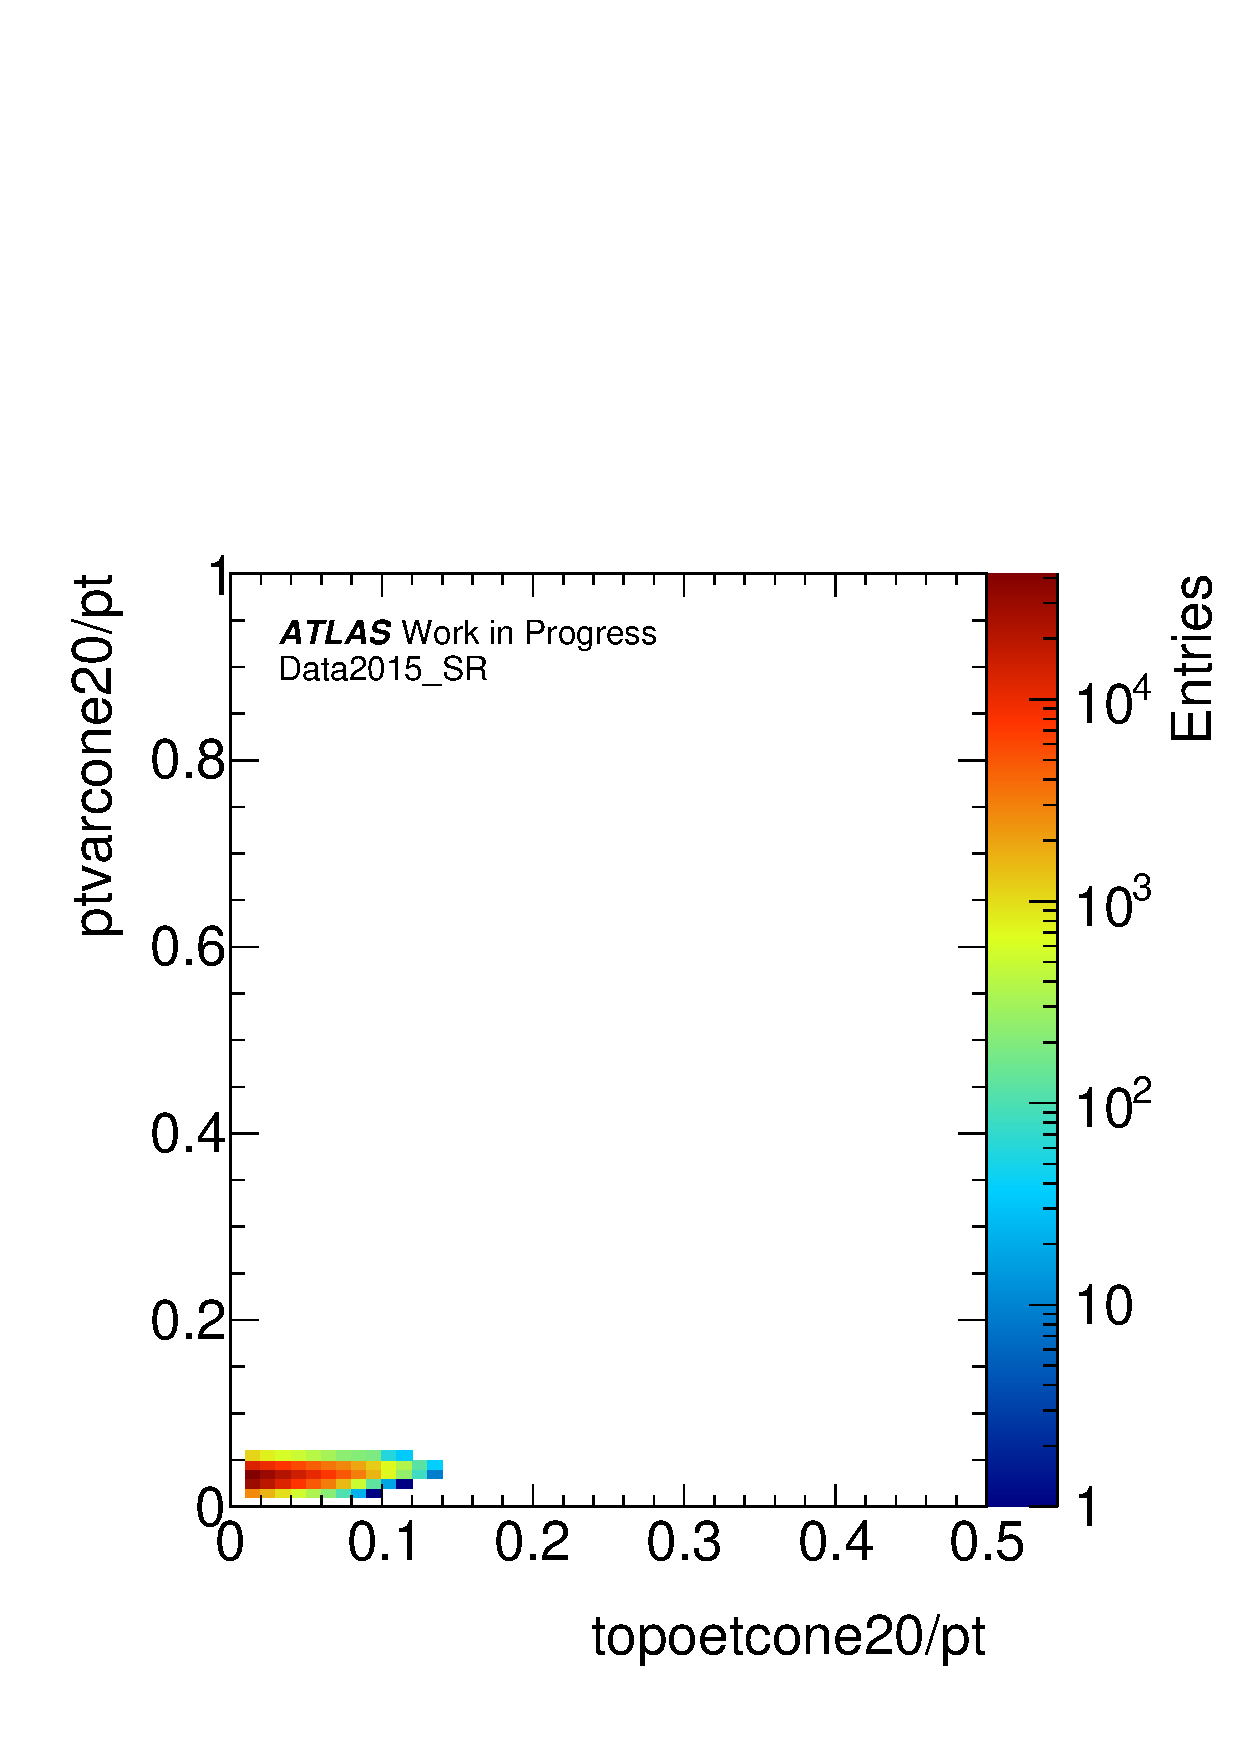
\includegraphics[width=0.4\textwidth]{figures/mj/plot2D-Data2015_SR-el_lep_0_iso_topoetcone20dPtVSel_lep_0_iso_ptvarcone20dPt-el.pdf}
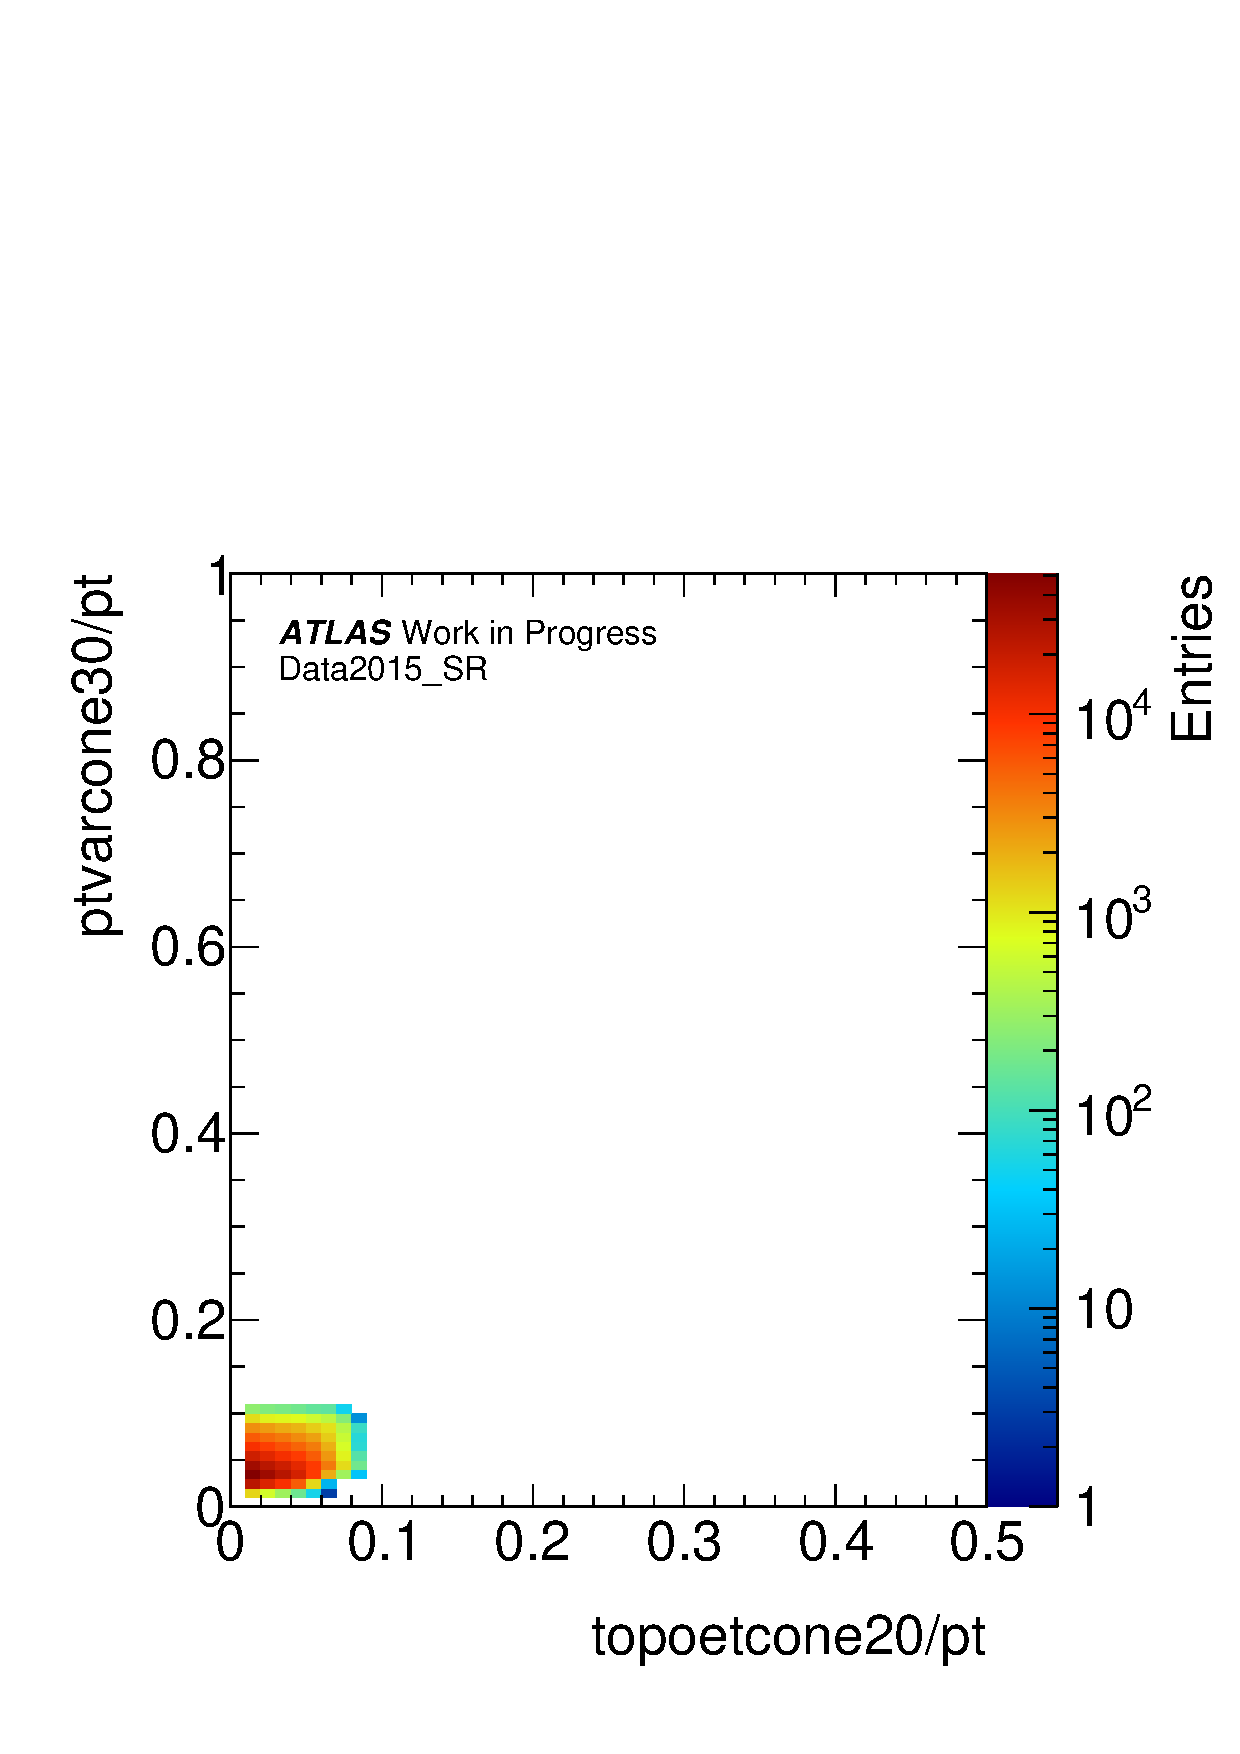
\includegraphics[width=0.4\textwidth]{figures/mj/plot2D-Data2015_SR-mu_lep_0_iso_topoetcone20dPtVSmu_lep_0_iso_ptvarcone30dPt-mu.pdf}
\\
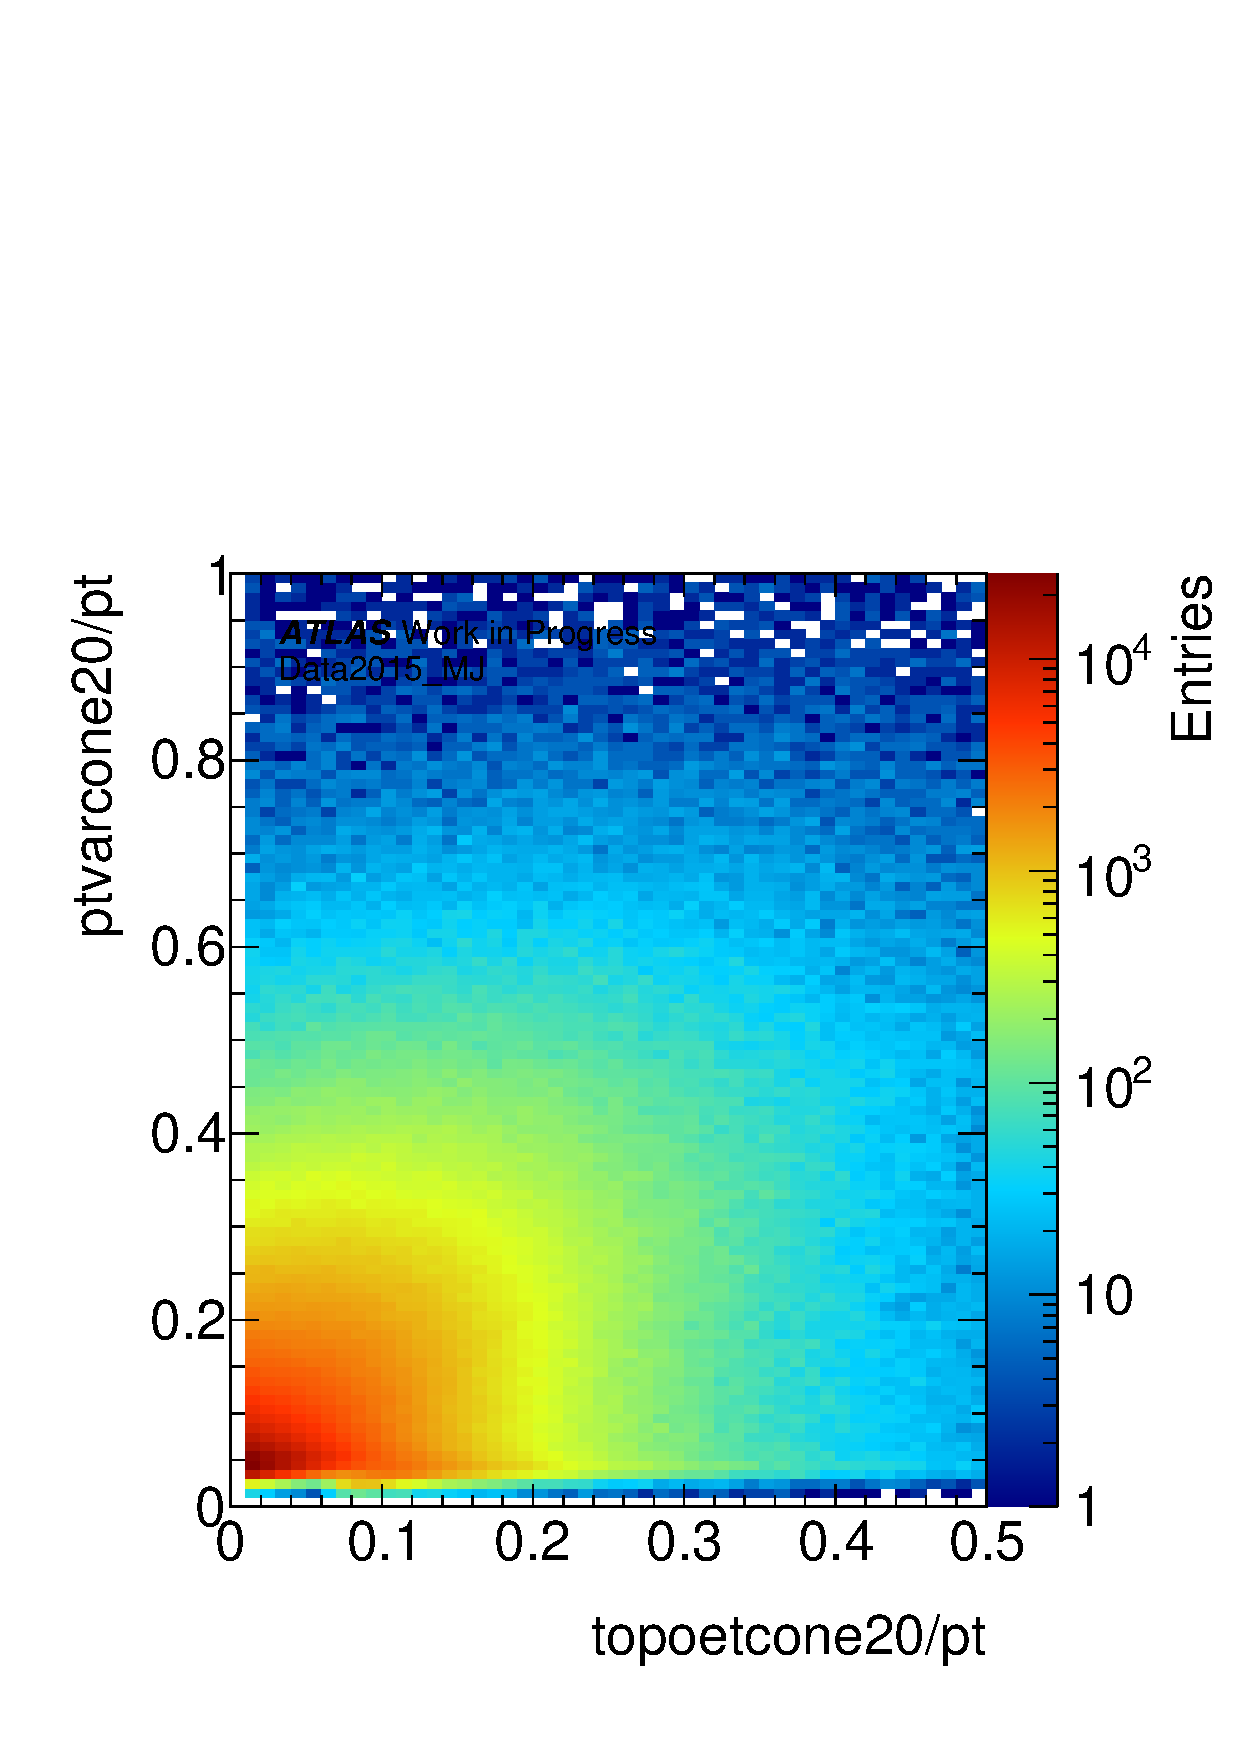
\includegraphics[width=0.4\textwidth]{figures/mj/plot2D-Data2015_MJ-el_lep_0_iso_topoetcone20dPtVSel_lep_0_iso_ptvarcone20dPt-el.pdf}
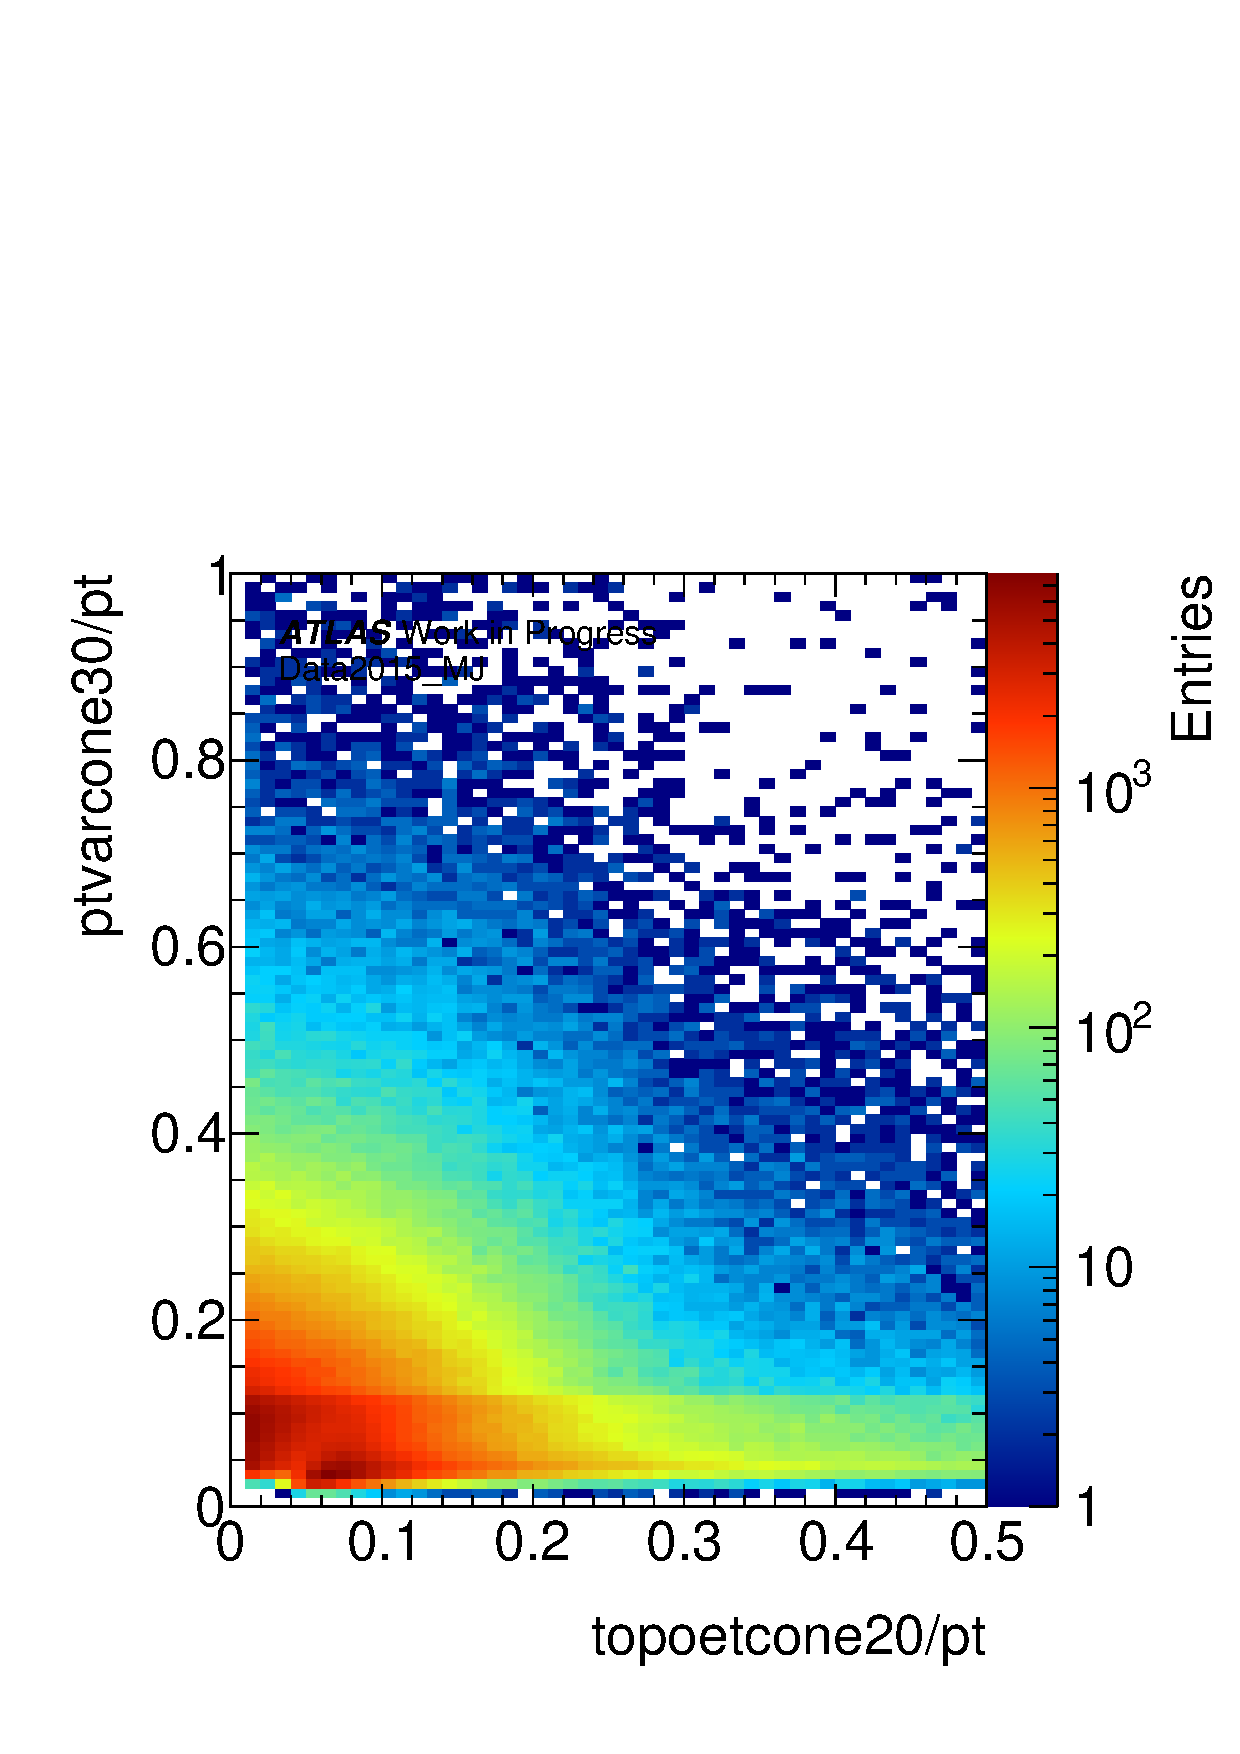
\includegraphics[width=0.4\textwidth]{figures/mj/plot2D-Data2015_MJ-mu_lep_0_iso_topoetcone20dPtVSmu_lep_0_iso_ptvarcone30dPt-mu.pdf}
\caption{
 Distribution of ptvarcone20(30)/$p_T$ versus topoetcone20/$p_T$ for electrons (left) and muons (right) for events passing (top) or failing (bottom) the Gradient-Iso selection in the data.
}
\label{fig:isolation_2D}
\end{figure}

As the Gradient-Iso phase space is only in a rectangular region of ptvarconeXX/$p_T$ versus topoetcone20/$p_T$, we decided to scan in slices of one isolation requirement at the time applying a fix cut on the other requirement to avoid biases from very non isolated events. 
The distribution of events failing the Gradient-Iso selection shown in Fig. \ref{fig:isolation_2D} gives also indication of the possible scan range and statistics of the scan  slices.

The fit was performed in two separate regions (fir regions - FR’s) defined removing in one case the $m_T^W > 40$ GeV cut, and in the other case removing the $E_T^{miss} > 25$ GeV cut.
In each fit region, fits are performed on following four variables: $p_T^{\ell}$, $E_T^{miss}$, $m_T^{W}$ and $\Delta \varphi _{\ell,E_T^{miss}}$ for each of the scan points, and the fraction of MJ is estimated extrapolating back to the signal region (re-applying the $m_T^W > 40$ GeV cut in one case, and the $E_T^{miss} > 25$ GeV cut in the other).
The contamination in each of the template regions, coming from the signal and the EW+top backgrounds varies a lot depending on the scan region.
A detailed description of such contaminations is reported in Table \ref{tbl:mj_ewk_bkg_fraction} and \todo{54}.

The stability of the MJ extraction was checked in several ways: the width of the \todo{isolation scan slices was varied}, the variables were fit in \todo{reduced ranges of the histograms} to reduce the impact of mismodellings of the data/MC distributions, and the EW and top backgrounds were \todo{kept fixed} by considering a very small Gaussian constraint on them.
In all these tests, the MJ estimates scans \todo{resulted to be close to one another}, and significantly smaller than the spread in the extrapolation coming from the use of different fit variables.
The study corresponding to a variation of the normalisation constraint on the EWK and top background is documented in detail in \todo{Appendix K}.

\subsubsection{$W\rightarrow e\nu$ scan results}
\label{sec:bkg_mj_we_scan}

As discussed in Sec. \ref{sec:bkg_mj_approach}, the events passing the gradient isolation cut and the selection are confined in the region of ptvarcone20/$p_T$ < 0.06 and topoetcone20/$p_T$ < 0.13. 
For this reason scans on the two variables,after inverting the gradient isolation, are performed for the values reported in Table \ref{tbl:mj_scan_binning_el}.

\begin{table}[htbp]
\small
\begin{center}
 \begin{tabular}{ | c | c | c | } 
 \hline
 Scan variable & ptvarcone20/$p_T$ & topoetcone20/$p_T$ \\
 \hline 
 Fixed cut & topoetcone20/$p_T$ < 0.13 & ptvarcone20/$p_T$ < 0.06 \\
 \hline 
 Scan starting point & 0.06 & 0.13 \\
 Slice width & 0.09 & 0.045 \\
 Number of slices & 6 & 6 \\
 \hline 
\end{tabular}
\caption{
Width of scan slices and boundaries used for $W\rightarrow e\nu$ channel.
}%
\label{tbl:mj_scan_binning_el}
\end{center}
\end{table}

The results for topoetcone20/$p_T$ and ptvarcone20/$p_T$ scans, and in the two fit regions, performed on $E_T^{miss}$, $m_T$, $p_T$ and $\Delta\varphi_{e,E_T^{miss}}$ are reported in Fig.\ref{fig:mj_extrapolation_wenu} for the $W\rightarrow e\nu$ channel.
Notice that the $\Delta\varphi_{e,E_T^{miss}}$ variable is missing $E_T^{miss}$-FR scans because returning often nonphysical negative or zero MJ yiels because of the poor discrimination power of such variable after the $m_T$>40 GeV cut is applied.
The errors on each of the scan points are the errors from the template fit, taking into account the discrimination power of the variables, as well as the statistics of the MJ template, \todo{multiplied by the $\sqrt(\chi^2/NDoF)$}, to account for eventual mismodelling in the considered variables.
More details on the extraction of the numbers are reported in Appendix \ref{sec:details_on_multijet_background_estimate_in_the_Wenu_channel}.

\begin{figure}[htbp]
\centering
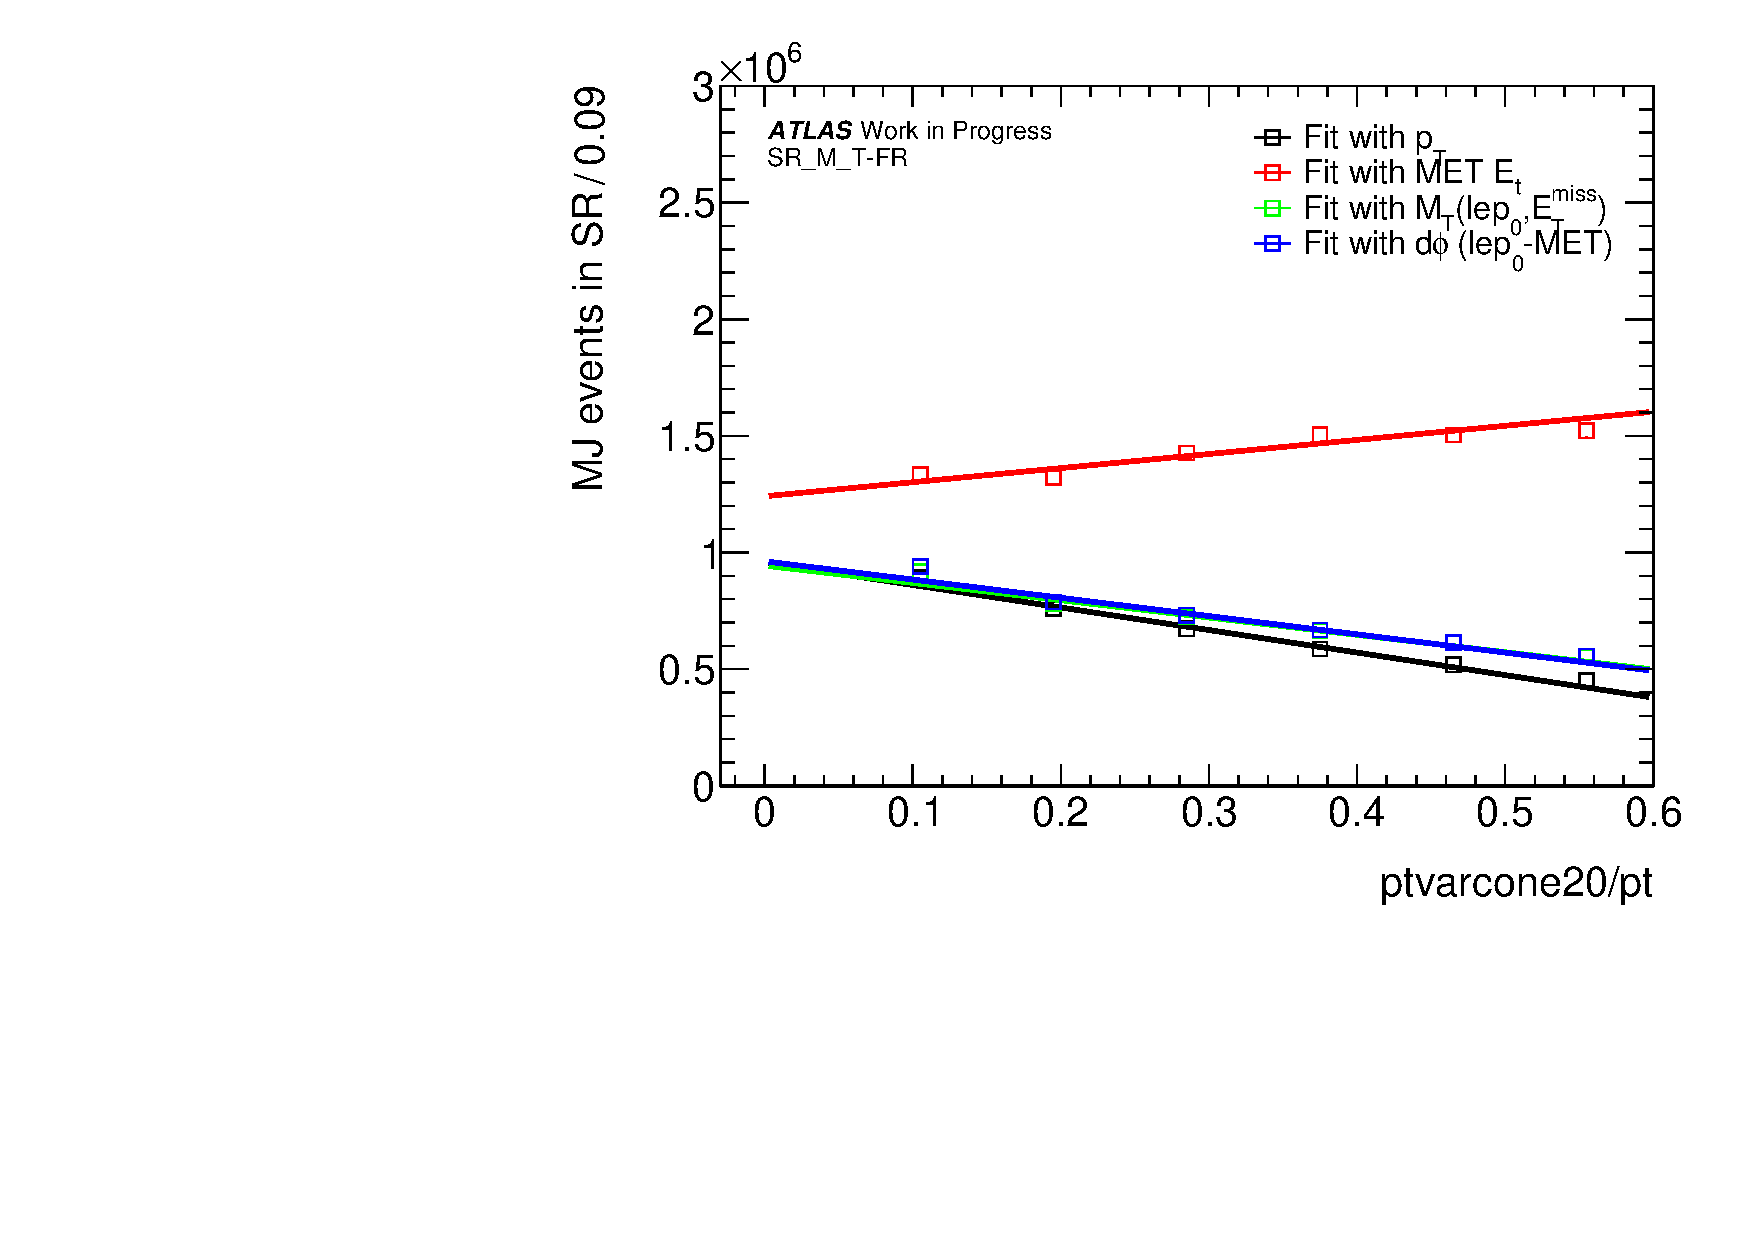
\includegraphics[width=0.45\textwidth]{figures/mj/slicesScanFit_SR_M_T_ptvar_el.pdf}
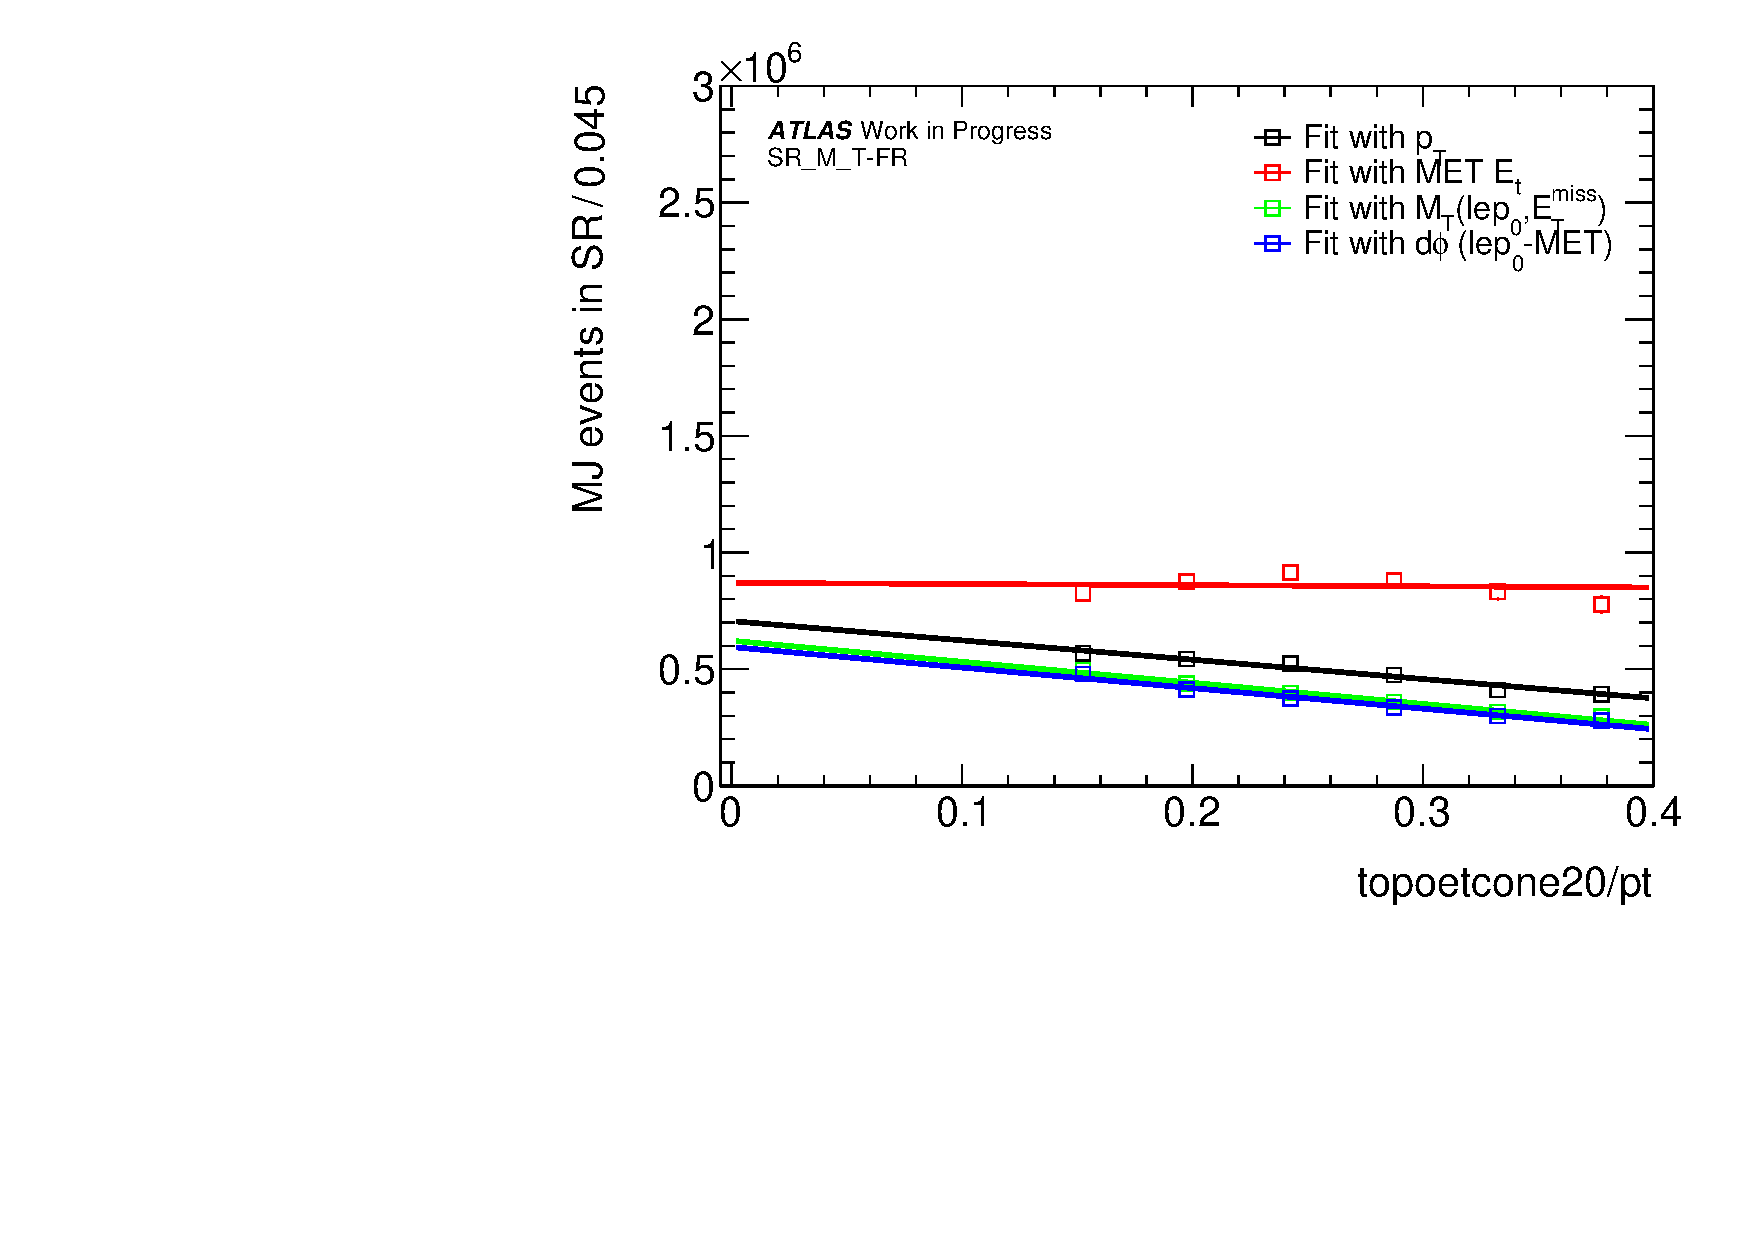
\includegraphics[width=0.45\textwidth]{figures/mj/slicesScanFit_SR_M_T_topoet_el.pdf}
\\
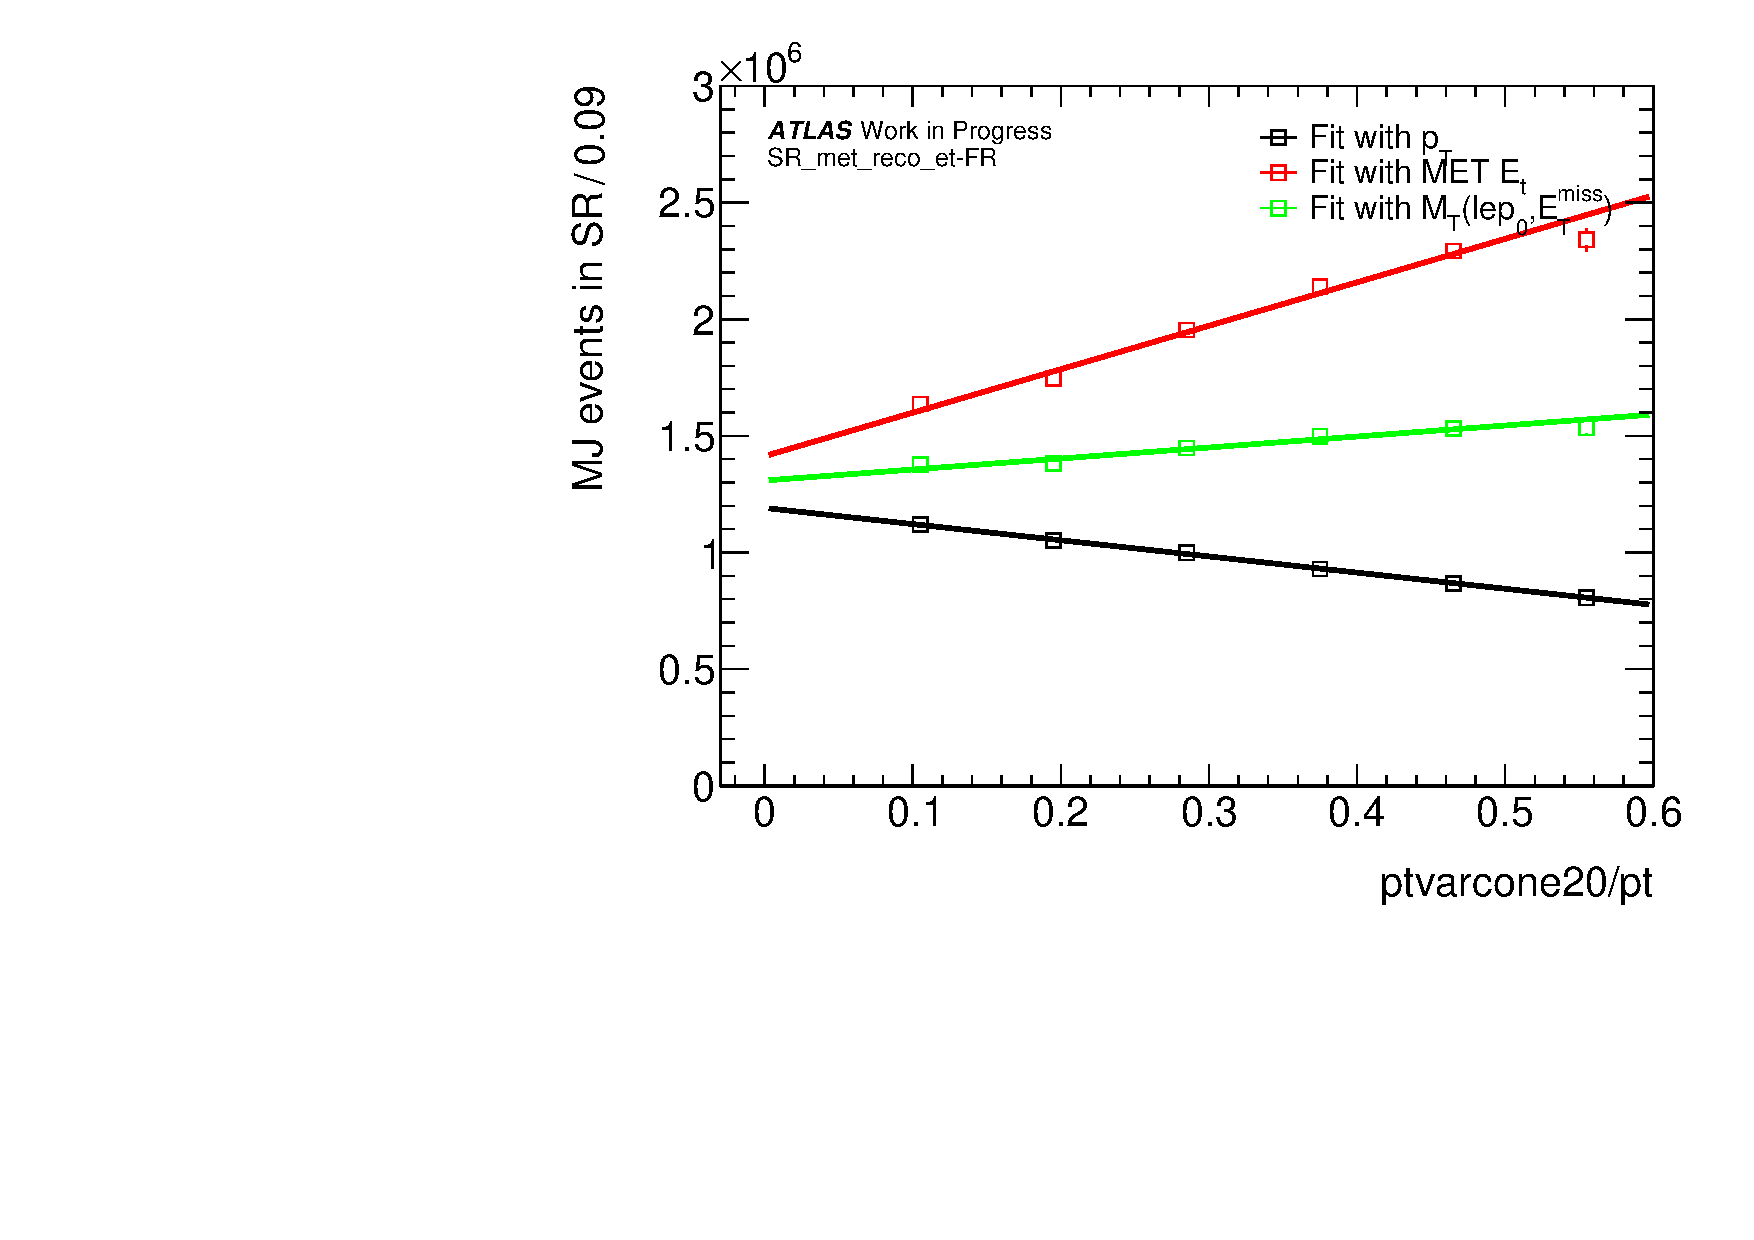
\includegraphics[width=0.45\textwidth]{figures/mj/slicesScanFit_SR_met_reco_et_ptvar_el.pdf}
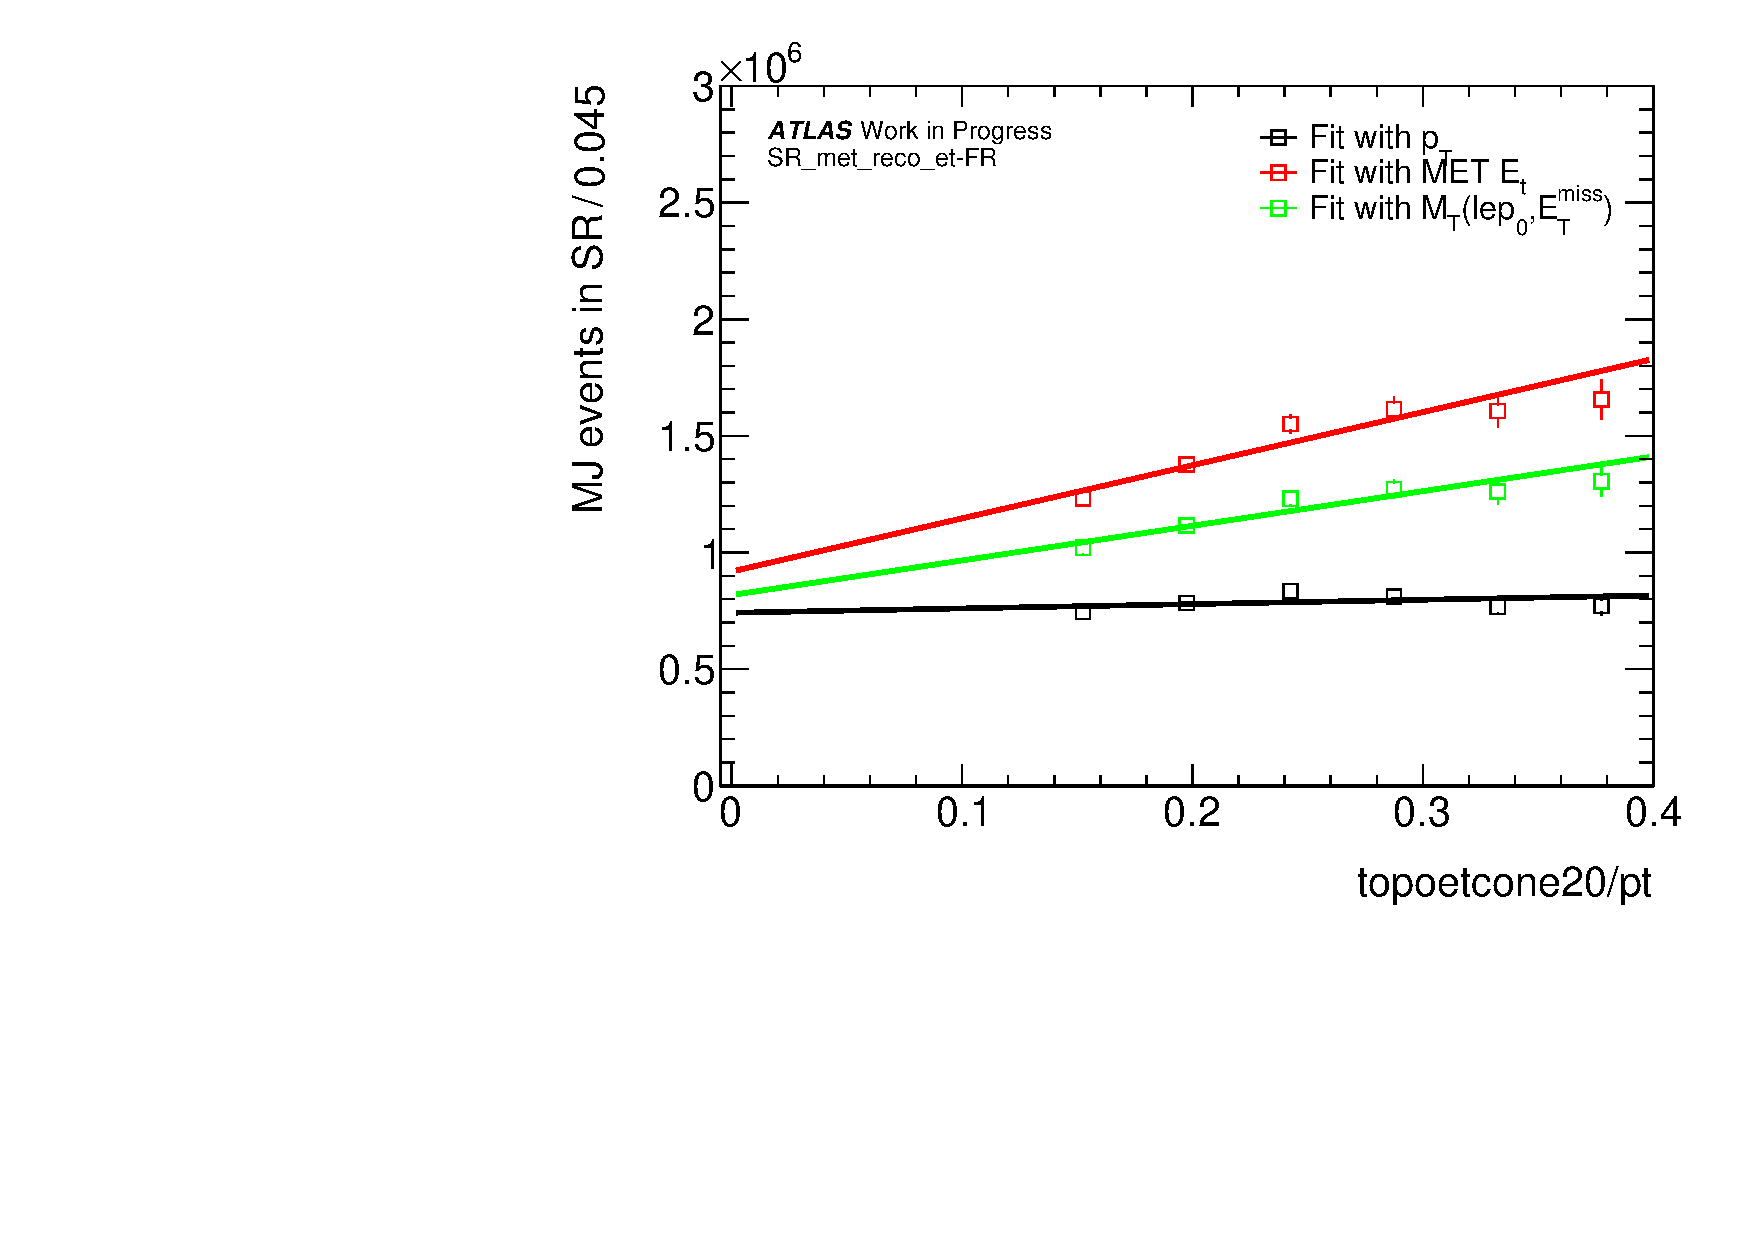
\includegraphics[width=0.45\textwidth]{figures/mj/slicesScanFit_SR_met_reco_et_topoet_el.pdf}
\caption{
 Plots of the scans for ptvarcone20/$p_T$ (left column) and topoetcone20/$p_T$ (right column) for the $W\rightarrow e\nu$ channel, $m_T$-FR (top raw), $E_T^{miss}$-FR (bottom row).
 The results relative to the scans of the different variables (fit in each slice and linear extrapolations) are shown in different colors: $E_T^{miss}$ (blue), $m_T$ (green), $p_T$ (red) and $\Delta\varphi_{e,E_T^{miss}}$ (black).
 Notice that the $\Delta\varphi_{e,E_T^{miss}}$ variable is missing $E_T^{miss}$-FR scans because 
 returning often nonphysical negative or zero MJ yiels because of the poor discrimination power of such variable after the $m_T$>40 GeV cut is applied.
 The errors on each of the scan points are the error from the template fit \todo{multiplied by the $\sqrt(\chi^2/NDoF)$}.
}
\label{fig:mj_extrapolation_wenu}
\end{figure}

In the plots it is visible the different behaviour of the variables, and their spread close to the signal region.
The fits performed on the $E_T^{miss}$ distribution have large error, coming mainly from the poor discriminating power of the $E_T^{miss}$.
Because of this the MJ extraction relative to the $E_T^{miss}$ has very large errors and central value relatively far from the one obtained with the other variables.
% The fits performed in the $E_T^{miss}$-relaxed fit region tend to \todo{give a slightly lower MJ estimate} with respect to the corresponding ones performed in the $m_T$-relaxed fit region.

The SR point of extrapolation is extracted from the average value of the ptvarcone20/$p_T$ and topoetcone20/$p_T$ distributions passing the gradient isolation selection cut in data (X and Y average of top left subfigure of Figure \ref{fig:isolation_2D}).
These values are \todo{0.034} and \todo{0.034} respectively.
The extrapolated values for $W\rightarrow e\nu$ for the topoetcone20/$p_T$ and ptvarcone20/$p_T$ respectively are reported in Table \ref{tbl:bkg_mj_we_scan_topoet} and \ref{tbl:bkg_mj_we_scan_ptvar}.
For details on the choice of the extrapolation values see \todo{Appendix P}.

\begin{table}[htbp]
\scriptsize
\begin{center}
 \begin{tabular}{ c | c  c | c  c } 
 \hline
Fit variable & MJ extrapolated SR\_met\_reco\_et-FR & $\chi^{2}$/NDoF of linear fit & MJ extrapolated SR\_M\_T-FR & $\chi^{2}$/NDoF of linear fit \\
\hline
\multicolumn{5}{c}{$W \rightarrow e \nu$} \\
\hline
$p_{T}$ & 741627.9 $\pm$ 34625.17 & 8.66/4 & 705913.9 $\pm$ 22912.59 & 3.99/4\\
$M_{T}(lep_{0},E^{miss}_{T})$ & 817560.7 $\pm$ 50581.89 & 5.95/4 & 621901.1 $\pm$ 18601.02 & 2.84/4\\
$d\phi (lep_{0}-MET)$ & - & -  & 594717.6 $\pm$ 17719.91 & 5.50/4\\
$MET E_{t}$ & 918511.4 $\pm$ 62436.09 & 8.67/4 & 869776.8 $\pm$ 37515.26 & 13.21/4\\
 \hline 
\end{tabular}
\caption{
Results of the extrapolation to the $W\rightarrow e\nu$ signal region (topoetcone20/$p_T$ = \todo{0.034}). 
The errors quoted come from the extrapolation at the SR points, varying in an anti-correlated way the $p_0$ and $p_1$ linear fit parameters of one $\sigma$.
}%
\label{tbl:bkg_mj_we_scan_topoet}
\end{center}
\end{table}

\begin{table}[htbp]
\scriptsize
\begin{center}
 \begin{tabular}{ c | c  c | c  c } 
 \hline
Fit variable & MJ extrapolated SR\_met\_reco\_et-FR & $\chi^{2}$/NDoF of linear fit & MJ extrapolated SR\_M\_T-FR & $\chi^{2}$/NDoF of linear fit \\
\hline
\multicolumn{5}{c}{$W \rightarrow e \nu$} \\
\hline
$p_{T}$ & 1191011.7 $\pm$ 7675.67 & 1.64/4 & 957321.2 $\pm$ 5624.70 & 57.39/4\\
$M_{T}(lep_{0},E^{miss}_{T})$ & 1308570.5 $\pm$ 10281.96 & 14.57/4 & 943721.3 $\pm$ 5708.18 & 99.32/4\\
$d\phi (lep_{0}-MET)$ & - & -  & 962359.0 $\pm$ 5862.21 & 120.70/4\\
$MET E_{t}$ & 1413057.8 $\pm$ 13226.37 & 27.03/4 & 1240946.8 $\pm$ 11362.84 & 42.96/4\\
 \hline 
\end{tabular}
\caption{
Results of the extrapolation to the $W\rightarrow e\nu$ signal region (ptvarcone20/$p_T$ = \todo{0.034}). 
The errors quoted come from the extrapolation at the SR points, varying in an anti-correlated way the $p_0$ and $p_1$ linear fit parameters of one $\sigma$.
}%
\label{tbl:bkg_mj_we_scan_ptvar}
\end{center}
\end{table}

The final background yield and its systematic uncertainty are estimated from the spread of the extrapolated curves of the ptvarcone20/$p_T$ and topoetcone20/$p_T$ variables.
To obtain the central value of the estimate, the weighted averages of the extrapolated values are computed, separately for the topoetcone and ptvarcone scans, and each fitting region.
The weighted average is calculated taking into account as anti-correlated the uncertainties on the $p_0$ and $p_1$ parameters of the fitted lines.
The nominal MJ yield is taken as the average between the four weighted averages (from the different scan variables and FR’s), and is shown in Table \ref{tbl:bkg_mj_we_wa_total}.
Seven sources of uncertainties, detailed in Table \ref{tbl:bkg_mj_we_wa_total}, are considered on the method:
\begin{itemize}
\item four come from the weighted average calculation, and are reported in Table \ref{tbl:bkg_mj_we_wa_extrapolation};
\item one represents the difference between the choice of scan variables, averaged over FR;
\item one represents the difference between the choice of FR, averaged over the scan variable;
\item one shows the \todo{impact of the JES variation on the signal template} in the estimated MJ yield.
\end{itemize}

\begin{table}[htbp]
\scriptsize
\begin{center}
 \begin{tabular}{ | c | c | c | c | c | } 
 \hline
Channel & \multicolumn{4}{|c|}{Weighted averages} \\
  & SR\_met\_reco\_et-FR, topoet Isol & SR\_met\_reco\_et-FR, ptvar Isol & SR\_M\_T-FR, topoet Isol & SR\_M\_T-FR, ptvar Isol \\
\hline
 $W \rightarrow e\nu$  & 792289.20 $\pm$ 25980.86 & 1265082.57 $\pm$ 5577.22 & 650620.41 $\pm$ 10727.11 & 976746.77 $\pm$ 3175.92 \\
  \hline
\end{tabular}
\caption{
Weighted average for $W\rightarrow e\nu$ in the two channels, for both scans and fit-regions (FR), with errors coming from the extrapolation.
}%
\label{tbl:bkg_mj_we_wa_extrapolation}
\end{center}
\end{table}

\begin{table}[htbp]
\scriptsize
\begin{center}
 \begin{tabular}{ | c | c | c | c | c | c | c | c | } 
\hline
Channel & \textbf{MJ yield} & \multicolumn{6}{|c|}{Systematic uncertanty} \\
 &  & $E_T^{miss}$-FR, topoet & $E_T^{miss}$-FR, ptvar & $m_T$-FR, topoet & $m_T$-FR, ptvar & scan choice & FR choice \\
\hline
 $W \rightarrow e\nu$  & \textbf{921184.74} & $\pm$ 1790.69 & $\pm$ 5577.22 & $\pm$ 10727.11 & $\pm$ 3175.92 & $\pm$ 747675.53 & $\pm$ 133213.48 \\
  \hline
\end{tabular}
\caption{
MJ estimated yield, obtained from averaging the weighted averages from the different scan variables and fit regions, and systematic uncertainties taken into account. 
The errors come from the extrapolations first four, the choice of scan variable, the choice of fit region, and \todo{shape variations} of the signal due to reconstruction systematics.
}%
\label{tbl:bkg_mj_we_wa_total}
\end{center}
\end{table}


The spread of the extrapolations from each scan is illustrated, in comparison with their weighted averages, and the final MJ estimated yield and total uncertainty, in Fig \ref{fig:mj_spread_extrapolations}.

\begin{figure}[htbp]
\centering
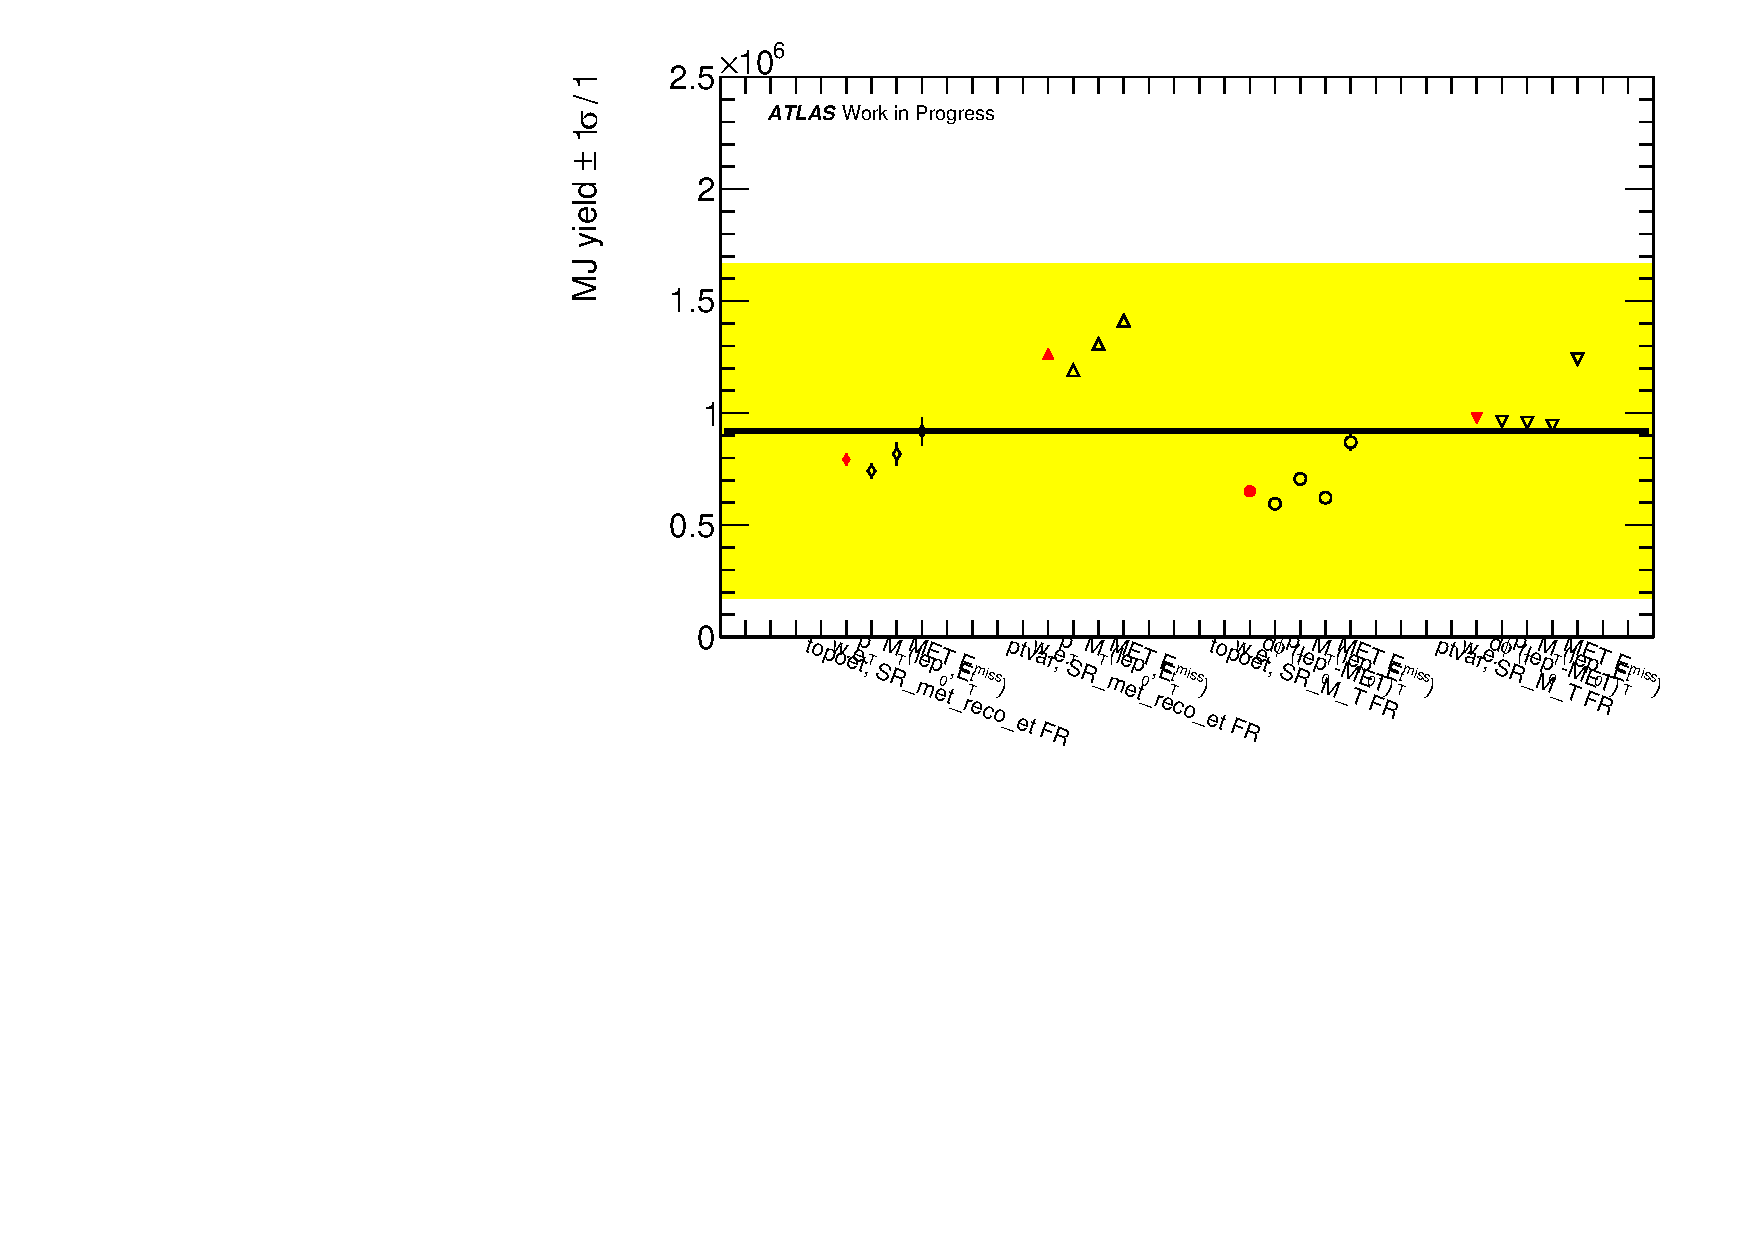
\includegraphics[width=0.75\textwidth]{figures/mj/spread_mj_el.pdf}
\caption{
 The spread of the extrapolations from each scan and their errors is illustrated with black empty markers, in comparison with their weighted averages, shown with red full markers, and the final MJ estimated yield (solid black line) and total uncertainty (yellow band), for each isolation scan variable, and fit region.
}
\label{fig:mj_spread_extrapolations}
\end{figure}

\subsubsection{$W\rightarrow\mu\nu$ scan results}
\label{sec:bkg_mj_wmu_scan}

As discussed in Sec. \ref{sec:bkg_mj_approach}, the events passing the gradient isolation cut and the selection are confined in the region of ptvarcone30/$p_T$ < 0.11 and topoetcone20/$p_T$ < 0.09. 
For this reason scans on the two variables, after inverting the gradient isolation, are performed for the values reported in Table \ref{tbl:bkg_mj_wmu_scan}. 
As for the electron channel, the scans in topoetcone20/$p_T$ are performed for a fixed range of ptvarcone30/$p_T$, so that the two sets of scans are orthogonal, the details are reported in Table \ref{tbl:bkg_mj_wmu_scan}.

\begin{table}[htbp]
\small
\begin{center}
 \begin{tabular}{ | c | c | c | } 
 \hline
 Scan variable & ptvarcone30/$p_T$ & topoetcone20/$p_T$ \\
 \hline 
 Fixed cut & topoetcone20/$p_T$ < 0.09 & ptvarcone30/$p_T$ < 0.11  \\
 \hline 
 Scan starting point & 0.11 & 0.09 \\
 Slice width & 0.11 & 0.44 \\
 Number of slices & 4 & 5 \\
 \hline 
\end{tabular}
\caption{
Width of scan slices and boundaries used for $W\rightarrow \mu\nu$ channel.
}%
\label{tbl:bkg_mj_wmu_scan}
\end{center}
\end{table}

The results for the scans, separated for the two variables and two fit regions, are shown in Fig.\ref{fig:mj_extrapolation_wmunu} for $W\rightarrow e\nu$ channel.
The errors on each of the scan points are the errors from the template fit, taking into account the discrimination power of the variables, as well as the statistics of the MJ template, multiplied by the $\sqrt(\chi^2/NDoF)$, to account for eventual mismodelling in the considered variables.
More details on the extraction of the numbers are reported in Appendix \ref{sec:details_on_multijet_background_estimate_in_the_Wmunu_channel}.

\begin{figure}[htbp]
\centering
\includegraphics[width=0.45\textwidth]{figures/intro/rdrds_summer18.png}
\includegraphics[width=0.45\textwidth]{figures/intro/rdrds_summer18.png}
\\
\includegraphics[width=0.45\textwidth]{figures/intro/rdrds_summer18.png}
\includegraphics[width=0.45\textwidth]{figures/intro/rdrds_summer18.png}
\caption{
 Plots of the scans for ptvarcone30/$p_T$ (left column) and topoetcone20/$p_T$ (right column) for the $W\rightarrow \mu\nu$ channel, $m_T$-FR (top raw), $E_T^{miss}$-FR (bottom row).
 The results relative to the scans of the different variables (fit in each slice and linear extrapolations) are shown in different colours: $E_T^{miss}$ (blue), $m_T$ (green), $p_T$ (red) and $\Delta\varphi_{\mu,E_T^{miss}}$ (black).
%  Notice that the $\Delta\varphi_{\mu,E_T^{miss}}$ variable is missing $E_T^{miss}$-FR scans because returning often nonphysical negative or zero MJ yiels because of the poor discrimination power of such variable after the $m_T$>40 GeV cut is applied.
 The errors on each of the scan points are the error from the template fit multiplied by the $\sqrt(\chi^2/NDoF)$.
}
\label{fig:mj_extrapolation_wmunu}
\end{figure}

The SR point of extrapolation is extracted from the average value of the ptvarcone30/$p_T$ and topoetcone20/$p_T$ distributions passing the gradient isolation selection cut in data (X and Y average of top right subfigure of Figure \ref{fig:isolation_2D}).
These values are \todo{0.045} and \todo{0.03} respectively.
The extrapolated values for $W\rightarrow e\nu$ for the topoetcone20/$p_T$ and ptvarcone20/$p_T$ respectively are reported in Table \ref{tbl:bkg_mj_wmu_scan_topoet} and \ref{tbl:bkg_mj_wmu_scan_ptvar}, together with the $\chi^2/NDoF$ for the linear extrapolations.
The errors quoted come from the extrapolation at the SR points, \todo{varying in an anti-correlated way} the $p_0$ and $p_1$ liner fit parameters of one $\sigma$.

\begin{table}[htbp]
\scriptsize
\begin{center}
 \begin{tabular}{ c | c  c | c  c } 
 \hline
Fit variable & MJ extrapolated SR\_met\_reco\_et-FR & $\chi^{2}$/NDoF of linear fit & MJ extrapolated SR\_M\_T-FR & $\chi^{2}$/NDoF of linear fit \\
\hline
\multicolumn{5}{c}{$W \rightarrow \mu \nu$} \\
 \hline
 \hline 
\end{tabular}
\caption{
Results of the extrapolation to the $W\rightarrow \mu\nu$ signal region (topoetcone20/$p_T$ = \todo{0.03}). 
The errors quoted come from the extrapolation at the SR points, varying in an anti-correlated way the $p_0$ and $p_1$ linear fit parameters of one $\sigma$.
}%
\label{tbl:bkg_mj_wmu_scan_topoet}
\end{center}
\end{table}

\begin{table}[htbp]
\scriptsize
\begin{center}
 \begin{tabular}{ c | c  c | c  c } 
 \hline
Fit variable & MJ extrapolated SR\_met\_reco\_et-FR & $\chi^{2}$/NDoF of linear fit & MJ extrapolated SR\_M\_T-FR & $\chi^{2}$/NDoF of linear fit \\
\hline
\multicolumn{5}{c}{$W \rightarrow \mu \nu$} \\
 \hline
 \hline 
\end{tabular}
\caption{
Results of the extrapolation to the $W\rightarrow \mu\nu$ signal region (ptvarcone30/$p_T$ = \todo{0.045}). 
The errors quoted come from the extrapolation at the SR points, varying in an anti-correlated way the $p_0$ and $p_1$ linear fit parameters of one $\sigma$.
}%
\label{tbl:bkg_mj_wmu_scan_ptvar}
\end{center}
\end{table}

The final background yield and its systematic uncertainty are estimated from the spread of the extrapolated curves at 0.045 and 0.03 value of the ptvarcone30/$p_T$ and topoetcone20/$p_T$ variables.
To obtain the central value of the estimate, the weighted averages of the extrapolated values are computed, separately for the topoetcone and ptvarcone scans, and each fitting region.
The weighted average is calculated taking into account as anti-correlated the uncertainties on the $p_0$ and $p_1$ parameters of the fitted lines.
The nominal MJ yield is taken as the average between the four weighted averages (from the different scan variables and FR’s), and is shown in Table \ref{tbl:bkg_mj_wmu_wa_total}.
Seven sources of uncertainties, detailed in Table \ref{tbl:bkg_mj_wmu_wa_total}, are considered on the method:
\begin{itemize}
\item four come from the weighted average calculation, and are reported in Table \ref{tbl:bkg_mj_wmu_wa_extrapolation};
\item one represents the difference between the choice of scan variables, averaged over FR;
\item one represents the difference between the choice of FR, averaged over the scan variable;
\item one shows the \todo{impact of the JES variation on the signal template} in the estimated MJ yield.
\end{itemize}

\begin{table}[htbp]
\scriptsize
\begin{center}
 \begin{tabular}{ | c | c | c | c | c | } 
 \hline
Channel & \multicolumn{4}{|c|}{Weighted averages} \\
  & SR\_met\_reco\_et-FR, topoet Isol & SR\_met\_reco\_et-FR, ptvar Isol & SR\_M\_T-FR, topoet Isol & SR\_M\_T-FR, ptvar Isol \\
\hline
 
  \hline
\end{tabular}
\caption{
Weighted average for $W\rightarrow \mu\nu$ in the two channels, for both scans and fit-regions (FR), with errors coming from the extrapolation.
}%
\label{tbl:bkg_mj_wmu_wa_extrapolation}
\end{center}
\end{table}

\begin{table}[htbp]
\scriptsize
\begin{center}
 \begin{tabular}{ | c | c | c | c | c | c | c | c | } 
\hline
Channel & \textbf{MJ yield} & \multicolumn{6}{|c|}{Systematic uncertanty} \\
 &  & $E_T^{miss}$-FR, topoet & $E_T^{miss}$-FR, ptvar & $m_T$-FR, topoet & $m_T$-FR, ptvar & scan choice & FR choice \\
\hline

  \hline
\end{tabular}
\caption{
MJ estimated yield, obtained from averaging the weighted averages from the different scan variables and fit regions, and systematic uncertainties taken into account. 
The errors come from the extrapolations first four, the choice of scan variable, the choice of fit region, and \todo{shape variations} of the signal due to reconstruction systematics.
}%
\label{tbl:bkg_mj_wmu_wa_total}
\end{center}
\end{table}


\subsection{Treatment of correlations between $W^+$ and $W^-$ multijet estimates}
\label{sec:bkg_mj_WplusWminus}


\subsubsection{Template fit method}
\label{sec:bkg_mj_we_ff}

The multijet background expectation in the $W\rightarrow \ell\nu$ ($\ell=e,\mu$) channel is divided among heavy-quark decays, conversions, and hadrons faking leptons. 
Since it is very difficult to model these events in MC, a template derived from data with a modified lepton selection (control region) is used to fit the $W$ transverse missing energy ($E_T^{miss}$) distribution in the signal region.

In this method, an enriched multijet template is constructed by selecting events from data where one lepton that passes the loose likelihood identification criteria, fails the tight criteria.
% (electron from photons conversion may be isolated, but the TightLH identification criteria places a requirement on the number of expected inner detector B-Layer hits, reducing the presence of the conversion component in the signal region). 
% Moreover, signal electrons must pass the isolation {\fontfamily{txtt}\selectfont FCTight} working point as defined by the {\fontfamily{txtt}\selectfont IsolationSelectionTool}~\cite{EGammaIdentificationRun2} while multijet-template electrons must fail.

% \todo{Pass isolation for signal and fail for MJ leptons.}
% \todo{Apply MET rebuild using MJ template leptons.}
% \todo{Fix trigger selection for MJ template.}
% \todo{I'd expect to see more diff for plots \ref{fig:FR2_ff} and \ref{fig:SR_ff}!}
% \todo{Do we relax both cuts for FR1/MJ?}


% The signal selection uses a loose likelihood lepton trigger and, by selecting loose leptons with this trigger, one will observe a high suppression of loose leptons. 
% Because of this effect, a single lepton \todo{loose trigger is used instead}....


The template needs to be built with a discriminating variable that can separate the background from the
signal. 
In this case, the $W$ missing energy ( $E_{T}^{miss}$ ) is constructed using the selected lepton-like object and the missing energy in the event but, for the template, the minimum $E_{T}^{miss}$ of 25 GeV and $m_{T}^{W}$ of 40 GeV cuts – present in the signal selection – are not applied, giving access to the low $E_{T}^{miss}$ and $m_{T}^{W}$ region where the QCD background is dominant.

It is expected that some events from signal, electroweak processes and top background pass the control region selection causing a contamination in this sample. 
However, this can be estimated – and can be subtracted – by selecting events from Monte Carlo simulation of these processes that pass the control region selection. 
One can see the results of this technique in Figure~ \ref{fig:FR2_ff}, that shows the distributions of the events and the contamination. 
The contamination of signal and non-QCD background in electron channel is estimated to be about 5\% of the events in the template selection region (where no transverse mass and missing energy cuts are applied).
If we consider only events above the transverse mass cut of 40 GeV and missing energy above 25 GeV, then the contamination corresponds to about 10.2\% of the number of events in the QCD background estimation.

For muon channel the contamination of signal and non-QCD background in muon channel is estimated to be about 13.7\% of the events in the template selection region.
Considering only events above the transverse mass cut of 40 GeV and missing energy above 25 GeV, then the contamination corresponds to about 43.3\% of the number of events in the QCD background estimation.

\begin{figure}[h]
\centering
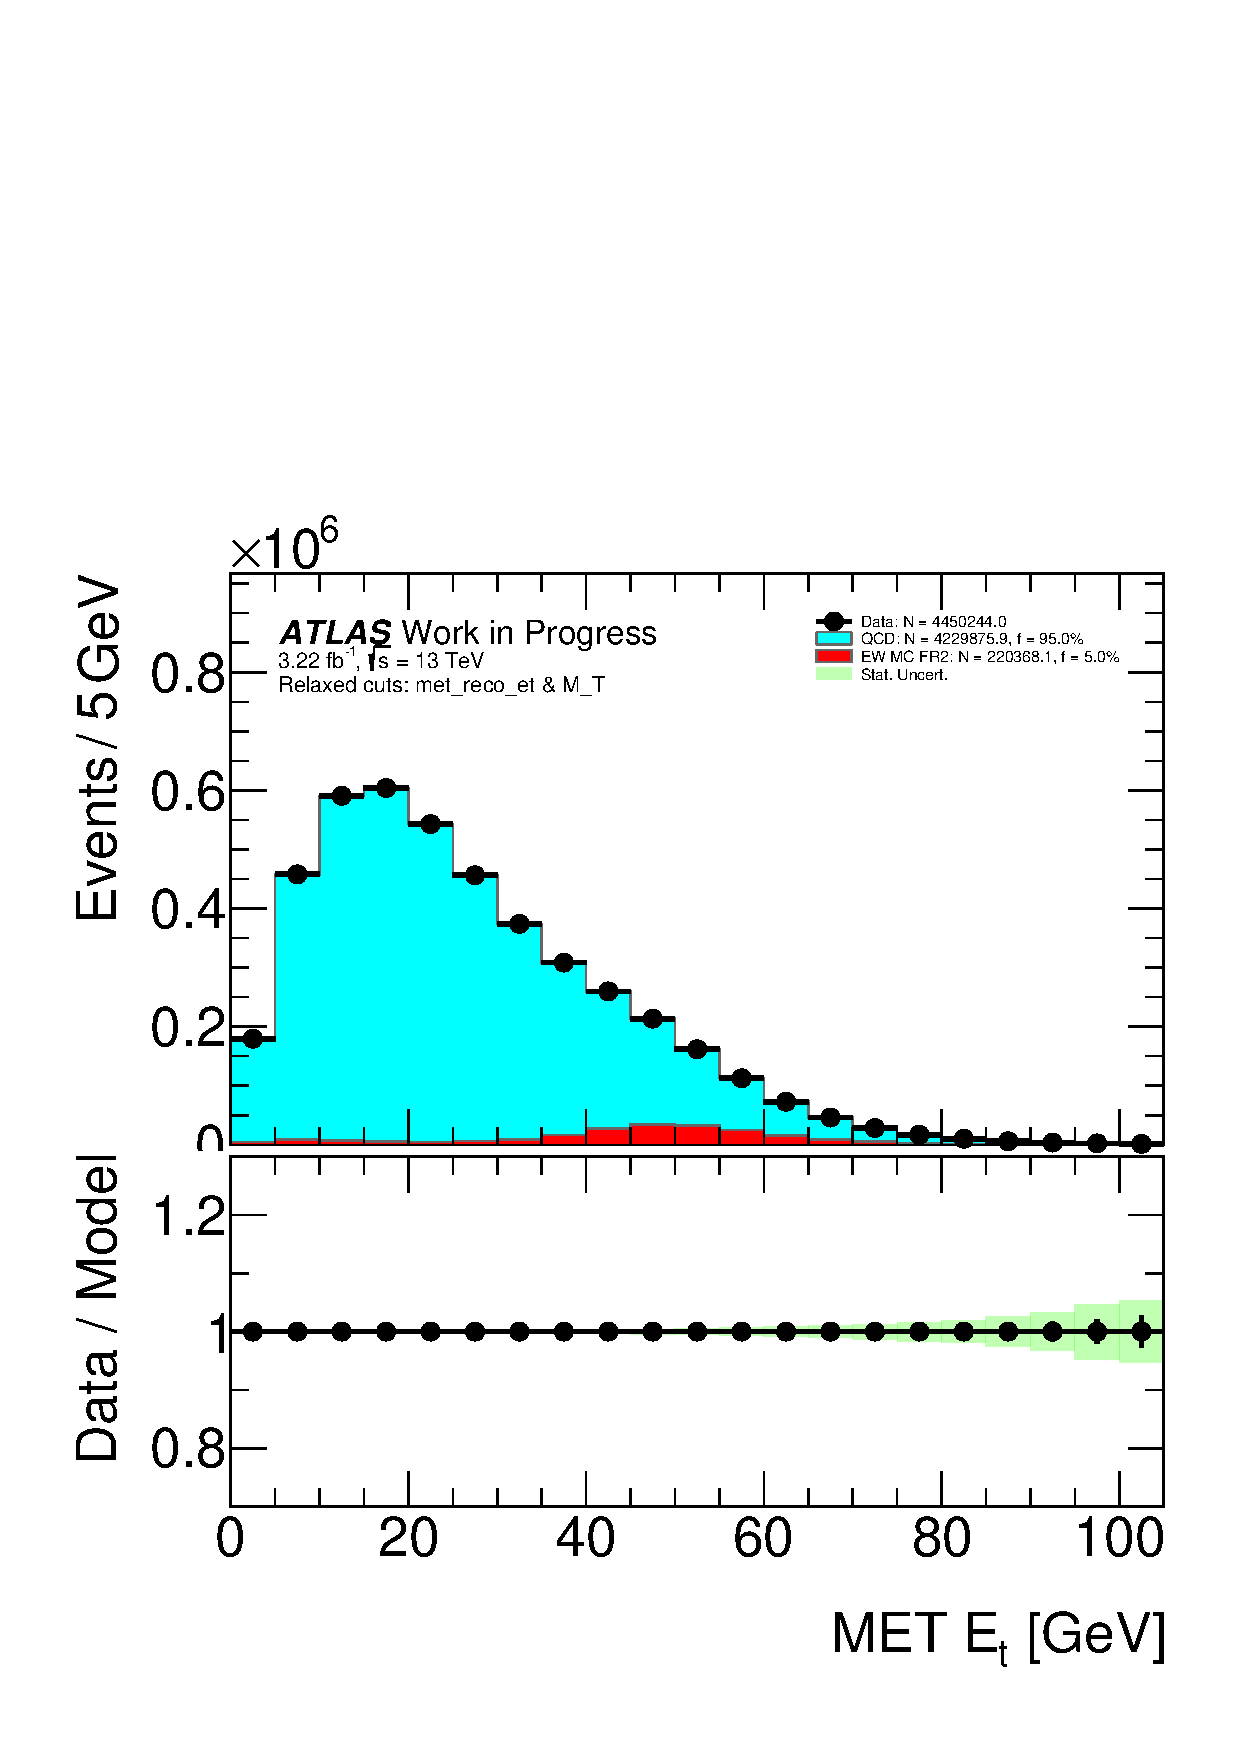
\includegraphics[width=0.45\textwidth]{figures/SR_MJ/fakeSlices-met_reco_et__M_T-AIso_AID-met_reco_et-antiIsoTight_FakeLepQual-FR2region-el.pdf}
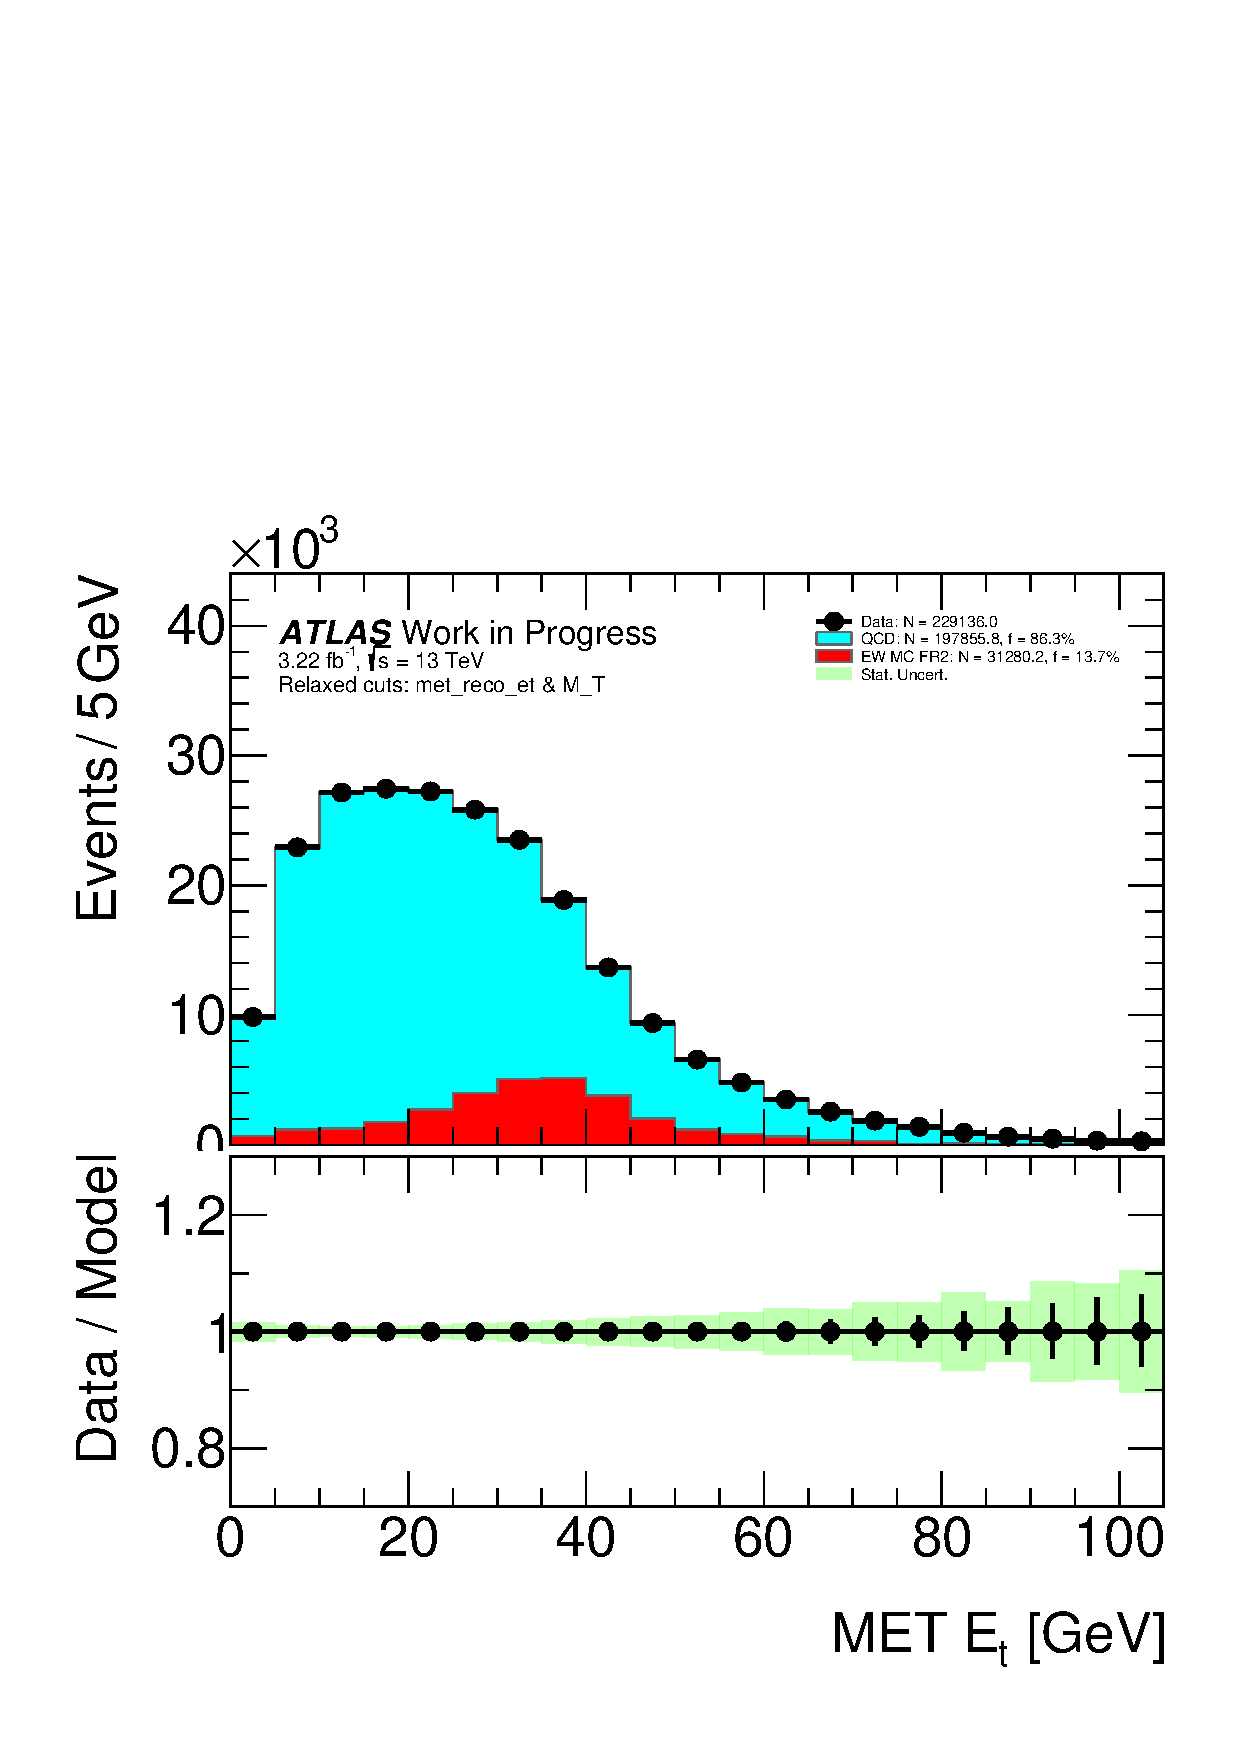
\includegraphics[width=0.45\textwidth]{figures/SR_MJ/fakeSlices-met_reco_et__M_T-AIso_AID-met_reco_et-antiIsoTight_FakeLepQual-FR2region-mu.pdf}
\caption{
The W transverse mass spectrum reconstructed in the electron (left) and muon (right) channel, for events passing the control region selection.
}
\label{fig:FR2_ff}
\end{figure}

A template fit on the W transverse missing energy is then performed, before applying the $m_{T}^{W} > 50$~GeV and $E_{T}^{miss}>25$~GeV cuts.
In the fit, the group of EWK processes and the multijet component are left free to float.
% , while the other backgrounds are constrained to their normalisation to the luminosity.
The template fit is performed for all events without any lepton charge selection.
The scale factors obtained from a fit are applied to the template described previously, where the contamination is subtracted, are shown on Fig.\ref{fig:FR1_ff}.
Then, an estimate of the fraction of multijet contamination in the signal region (SR) is obtained
using the fit scale factors and the data and MC templates with a cut on $m_{T}^{W} > 50$~GeV and $E_{T}^{miss}>25$~GeV.
The fractions of multijet background extrapolated to the signal region are displayed on Fig.~\ref{fig:SR_ff}.

Electron channel in  way more contaminated by multijet background then muon channel: fakes contribution is 10.5\% and 1.3\% respectively.
This is one more reason why we focus on the ratio of muons rather then electrons.

\begin{figure}[h]
\centering
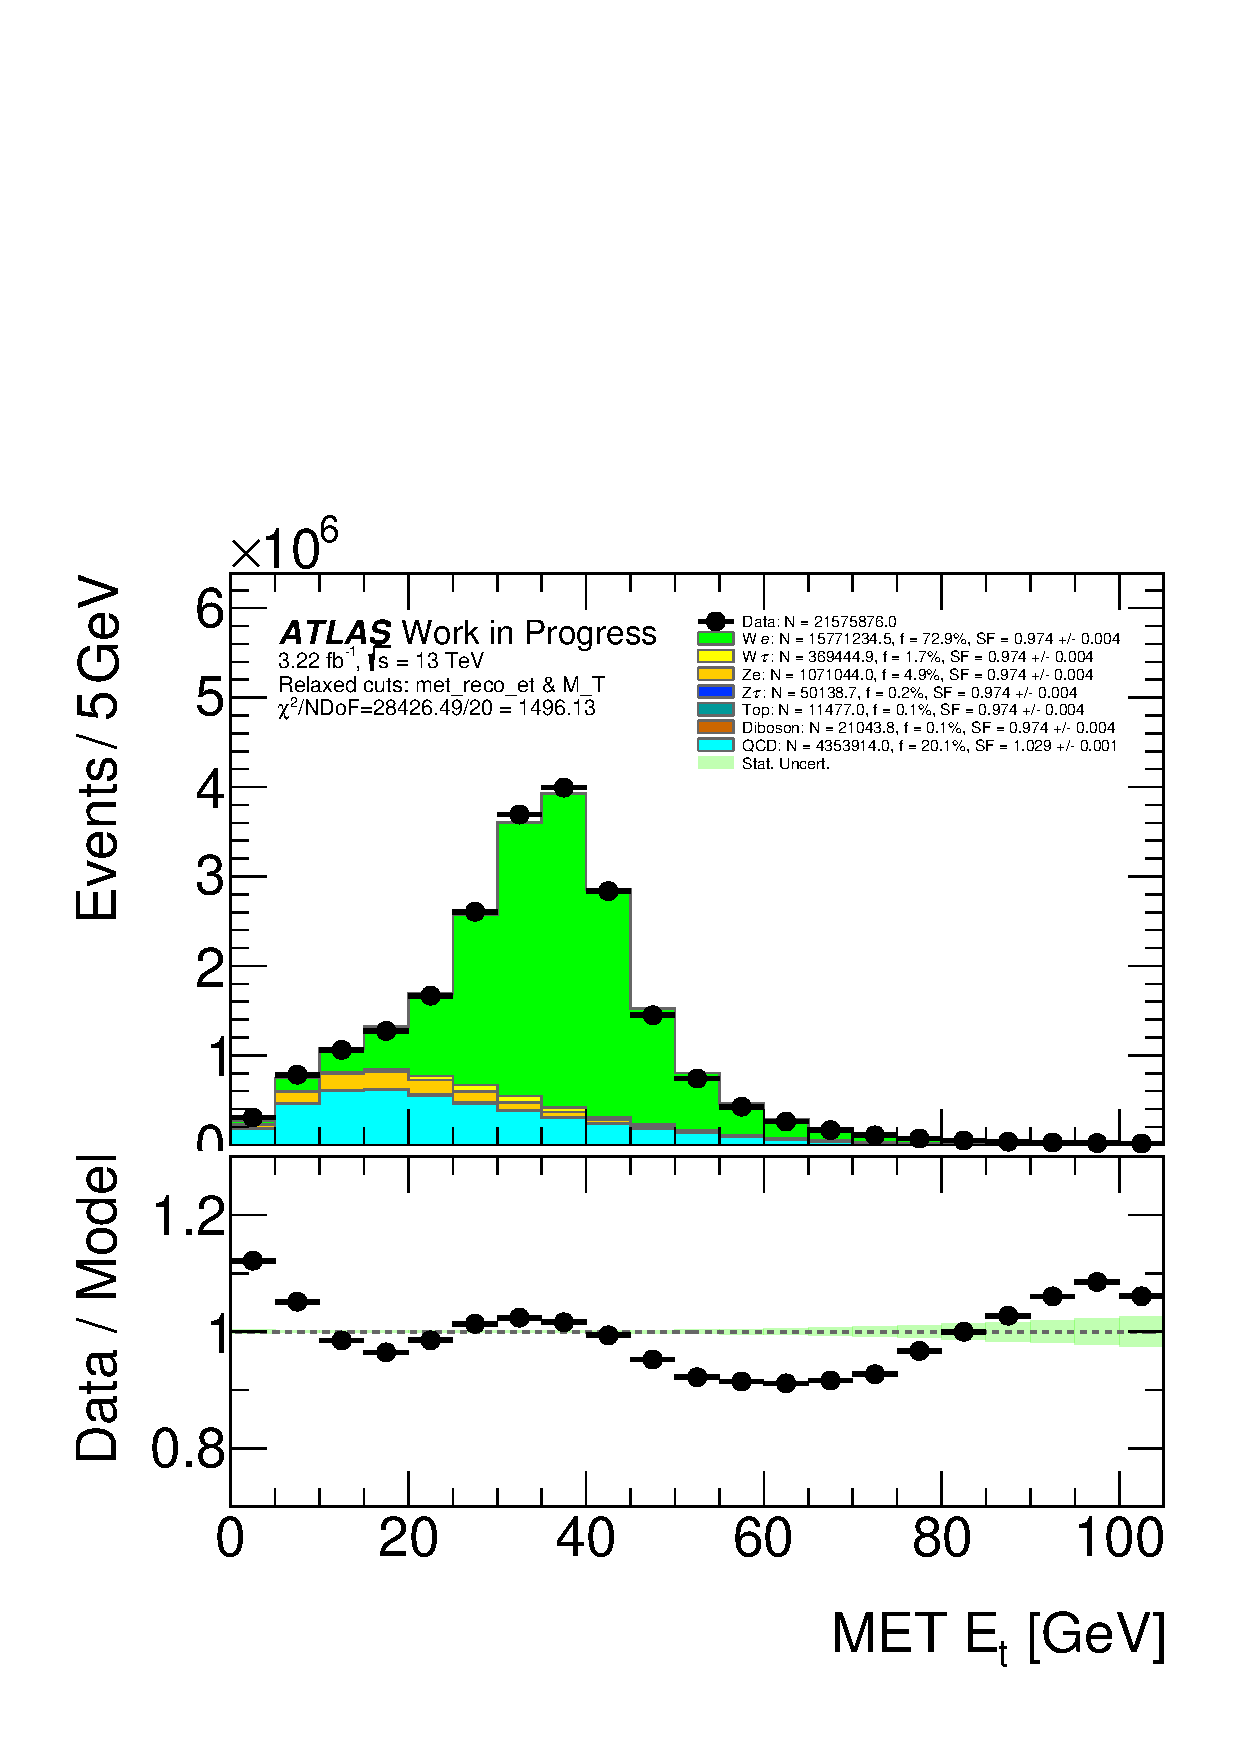
\includegraphics[width=0.45\textwidth]{figures/SR_MJ/fakeSlices-met_reco_et__M_T-AIso_AID-met_reco_et-antiIsoTight_FakeLepQual-FR1afterFit-el.pdf}
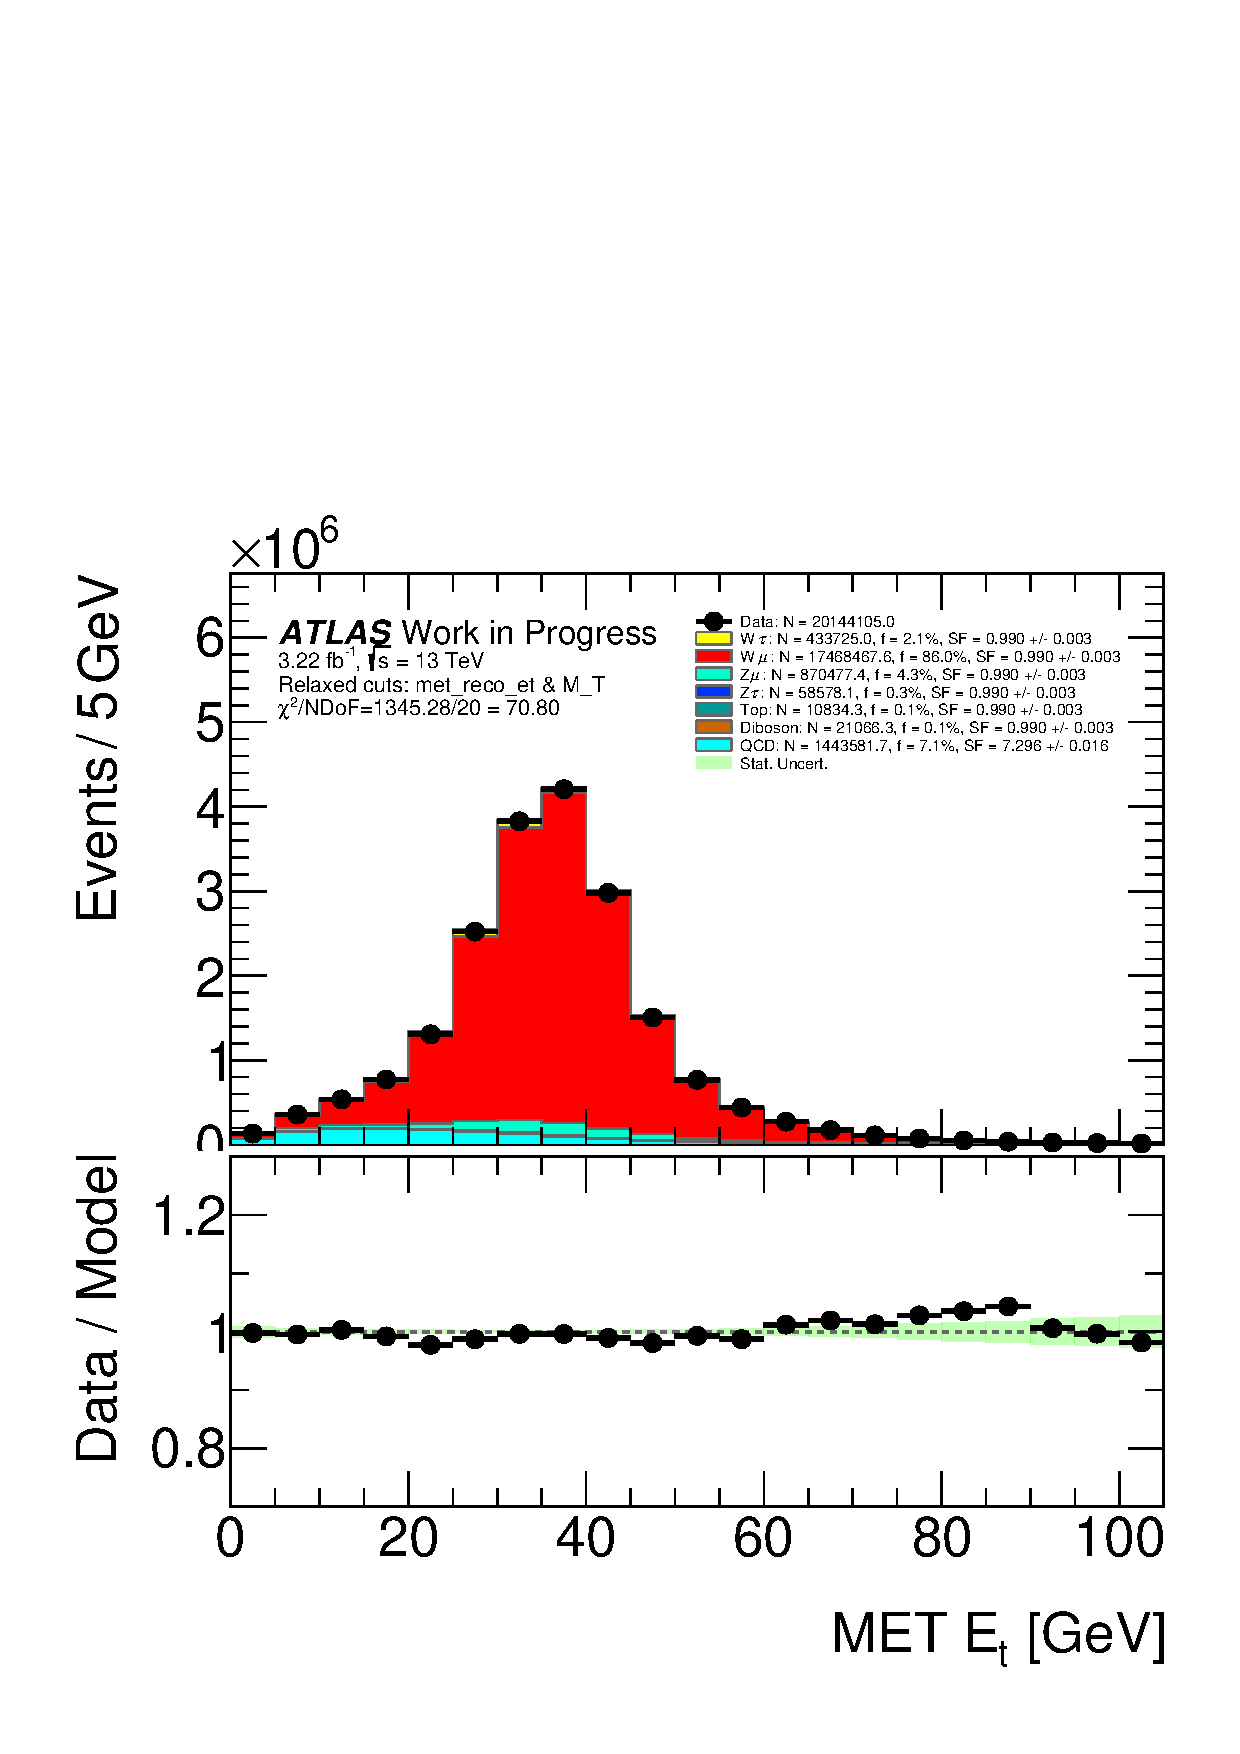
\includegraphics[width=0.45\textwidth]{figures/SR_MJ/fakeSlices-met_reco_et__M_T-AIso_AID-met_reco_et-antiIsoTight_FakeLepQual-FR1afterFit-mu.pdf}
\caption{
Results on the template fit to the full $m_{T}^{W}$ and $E_{T}^{miss}$ spectrum for signal and backgrounds, for $W\rightarrow e\nu$ (left) and for $W\rightarrow \mu\nu$ (right) channels, obtained from the template with inverted isolation and inverted likelihood identification criteria.
}
\label{fig:FR1_ff}
\end{figure}

\begin{figure}[h]
\centering
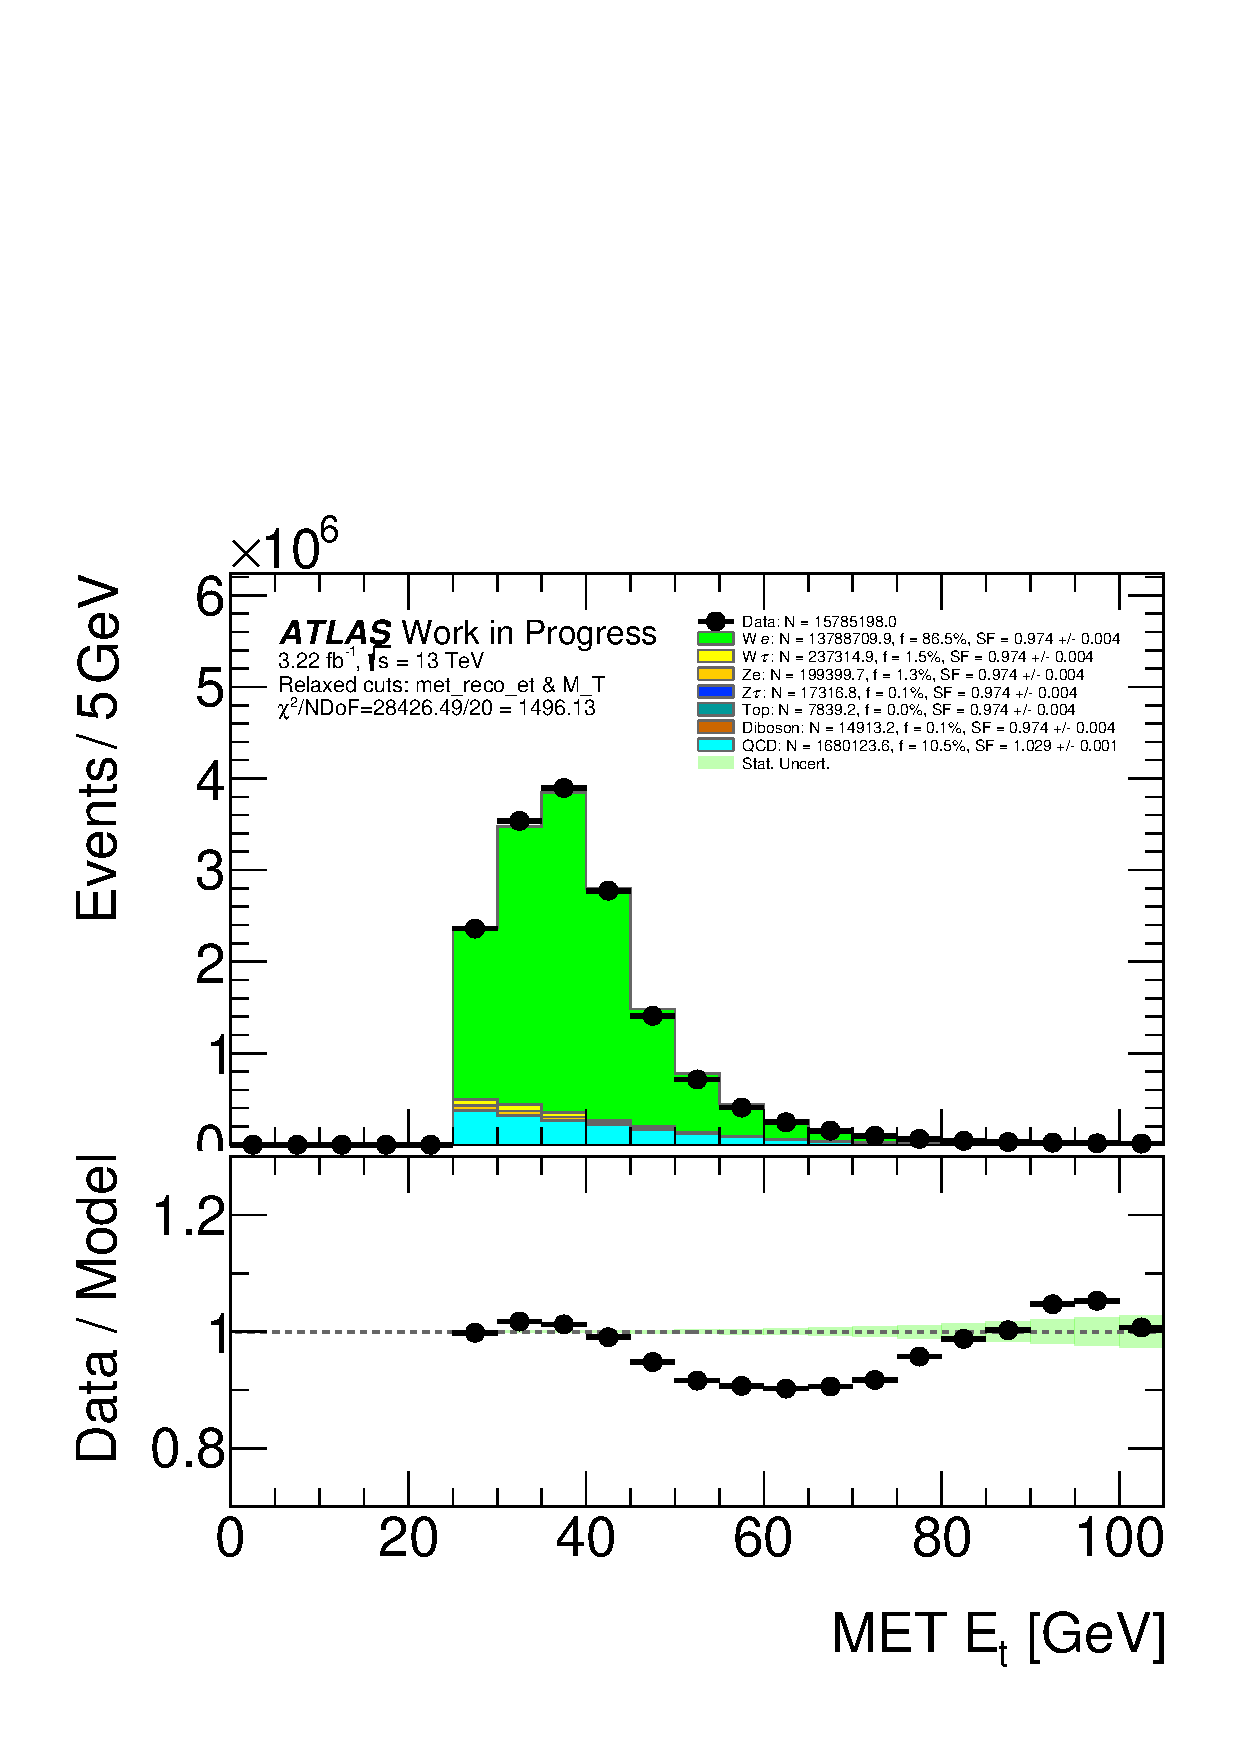
\includegraphics[width=0.45\textwidth]{figures/SR_MJ/fakeSlices-met_reco_et__M_T-AIso_AID-met_reco_et-antiIsoTight_FakeLepQual-SRafterFit-el.pdf}
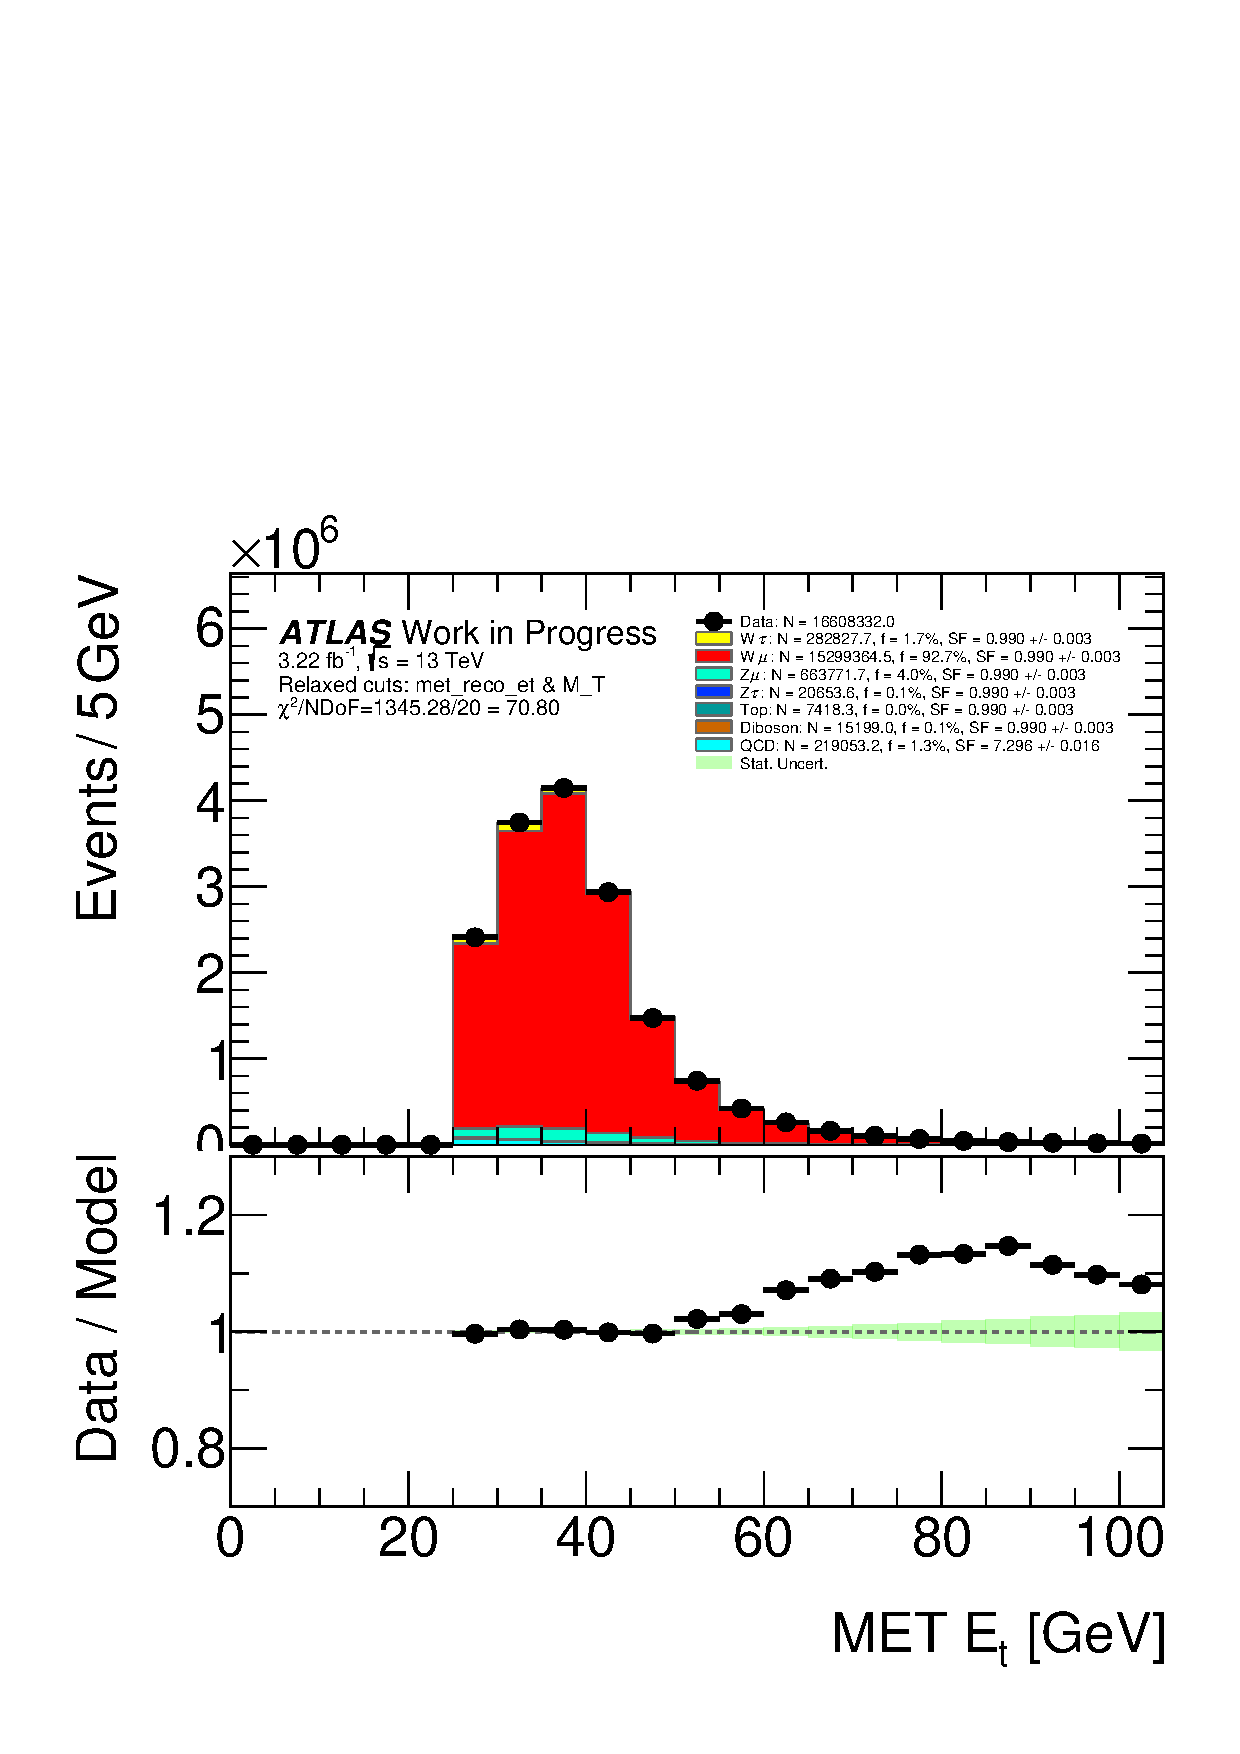
\includegraphics[width=0.45\textwidth]{figures/SR_MJ/fakeSlices-met_reco_et__M_T-AIso_AID-met_reco_et-antiIsoTight_FakeLepQual-SRafterFit-mu.pdf}
\caption{
Results on the of the multijet background template fit extrapolation to the signal region for signal and backgrounds, for $W\rightarrow e\nu$ (left) and for $W\rightarrow \mu\nu$ (right) channels, obtained from the template with inverted isolation and inverted likelihood identification criteria.
}
\label{fig:SR_ff}
\end{figure}





% %-------------------------------------------------------------------------------
% \section{Kinematic Distributions and Summary of background-subtracted Candidate Events}
% \label{sec:background_summary}
% %-------------------------------------------------------------------------------
% 
\subsection{Kinematic distributions}
\label{sec:kinematic_distributions}

Kinematic distributions for W and Z events passing the selection requirements described in Section~\ref{sec:event_selection} are presented in this section. 
The distributions for both $W \rightarrow e\nu$ and $W \rightarrow \mu\nu$, both inclusively and split in
charge, are shown in Figs.~\ref{fig:SR_lep_0_pt}-\ref{fig:SR_lepmet_dphi} while the equivalent distributions for both $Z \rightarrow e^+ e^-$ and $Z \rightarrow \mu^+ \mu^-$  are shown in Figs.~\ref{fig:ZR_lep_0_pt}-\ref{fig:ZR_dilep_eta}. 
The uncertainty bands shown in these distributions are described in Section~\ref{sec:background} and are calculated on the following components:
\begin{itemize}
% \item uncertainty due to the multijet background estimation method;
% \item lepton energy and momentum scale and resolution;
% \item lepton trigger efficiency;
% \item lepton reconstruction and identification efficiency, including uncertainties on lepton isolation;
% \item jet energy scale and resolution;
% \item soft (unclustered) energy contributions in the $E_{T}^{miss}$;
% \item uncertainties in cross section calculations for electroweak and top quark production; 
\item statistical uncertainty due to limited Monte Carlo sample sizes.
\end{itemize}

\todo{We don't have v10s04 MC samples in the GRID for sys calculations.} 
We'd expect to get sys calculations in the coming ntuple production.

% These uncertainties are included in the histograms as a shaded band, but the luminosity uncertainty of \todo{$\pm 5$\%} is explicitly omitted from such band.

% ##################
% SR
% ##################

\begin{figure}[htbp]
\centering
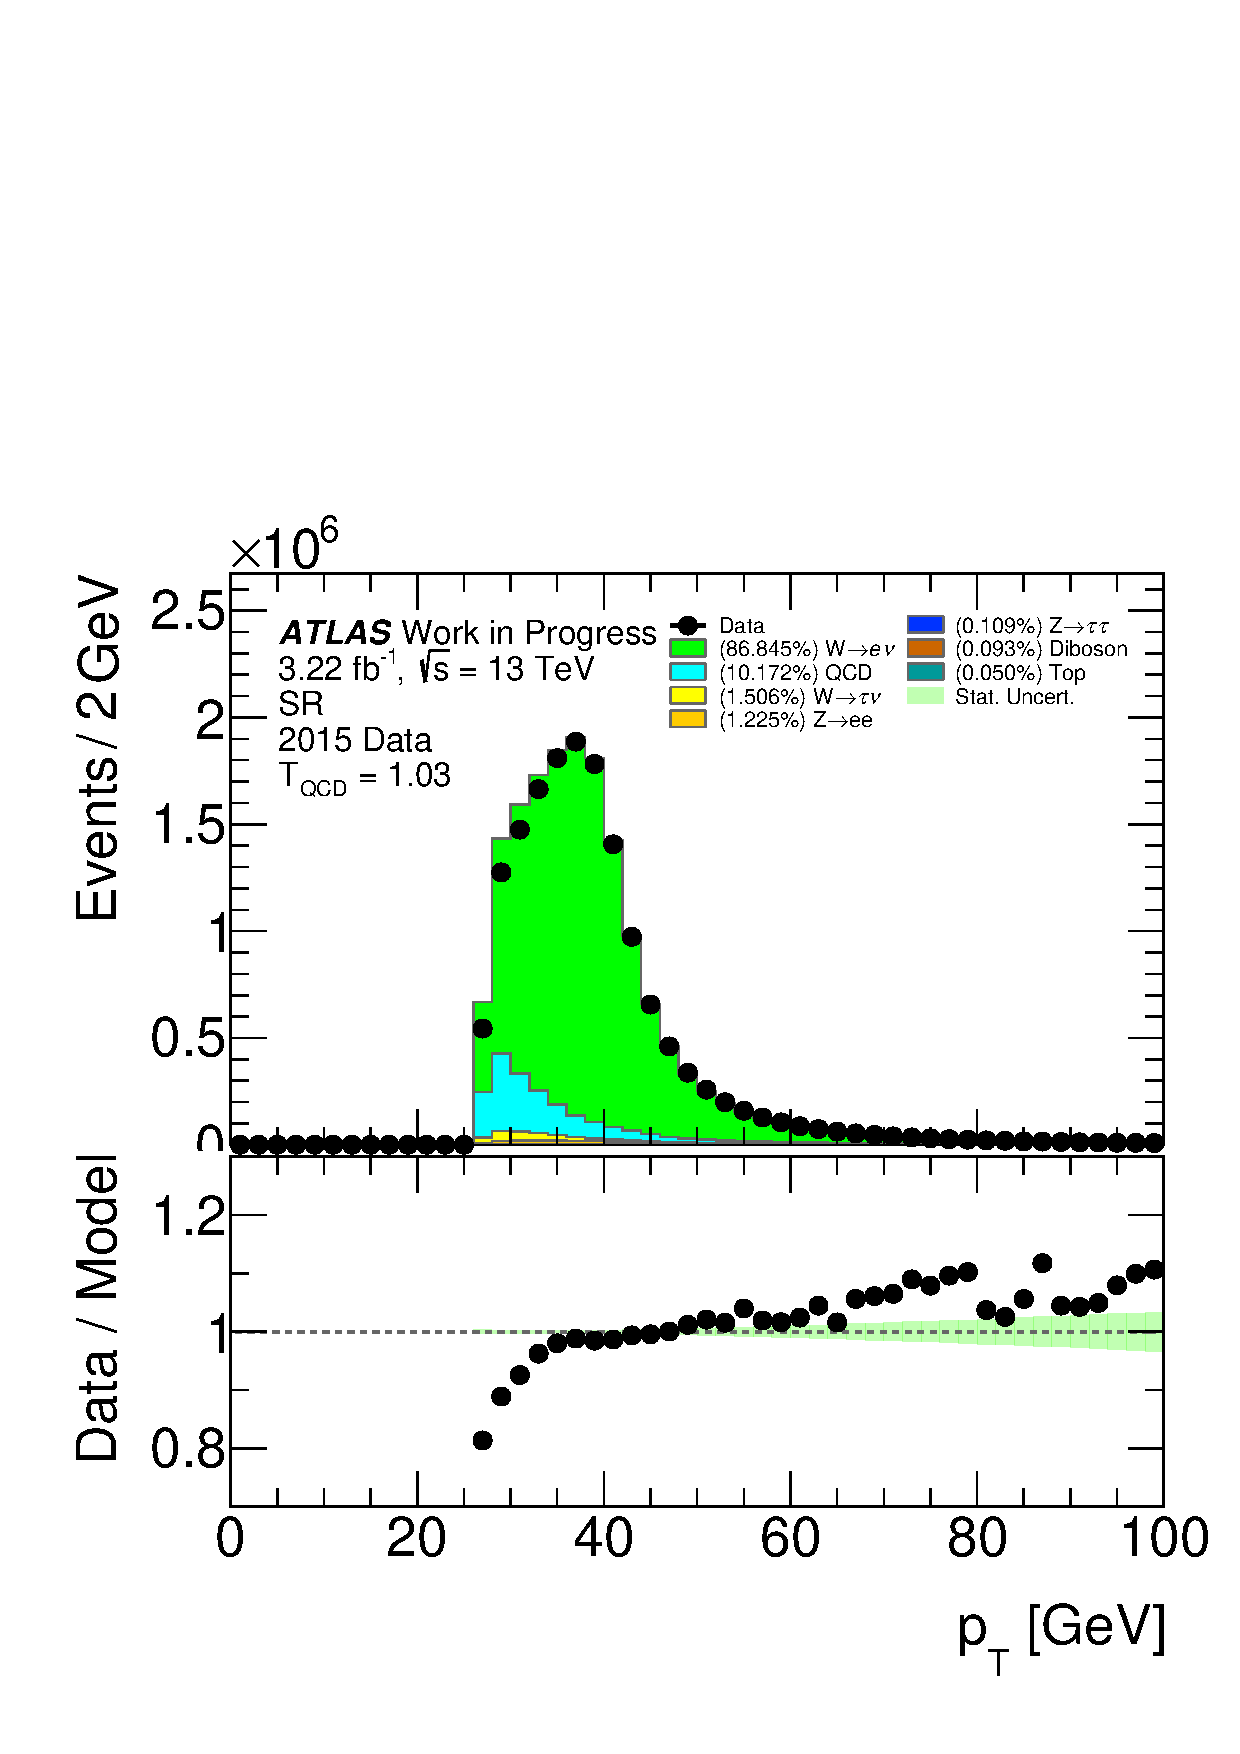
\includegraphics[width=0.45\textwidth]{figures/SR/dataMc-lep_0_pt-SR-bkgQCD-el.pdf}
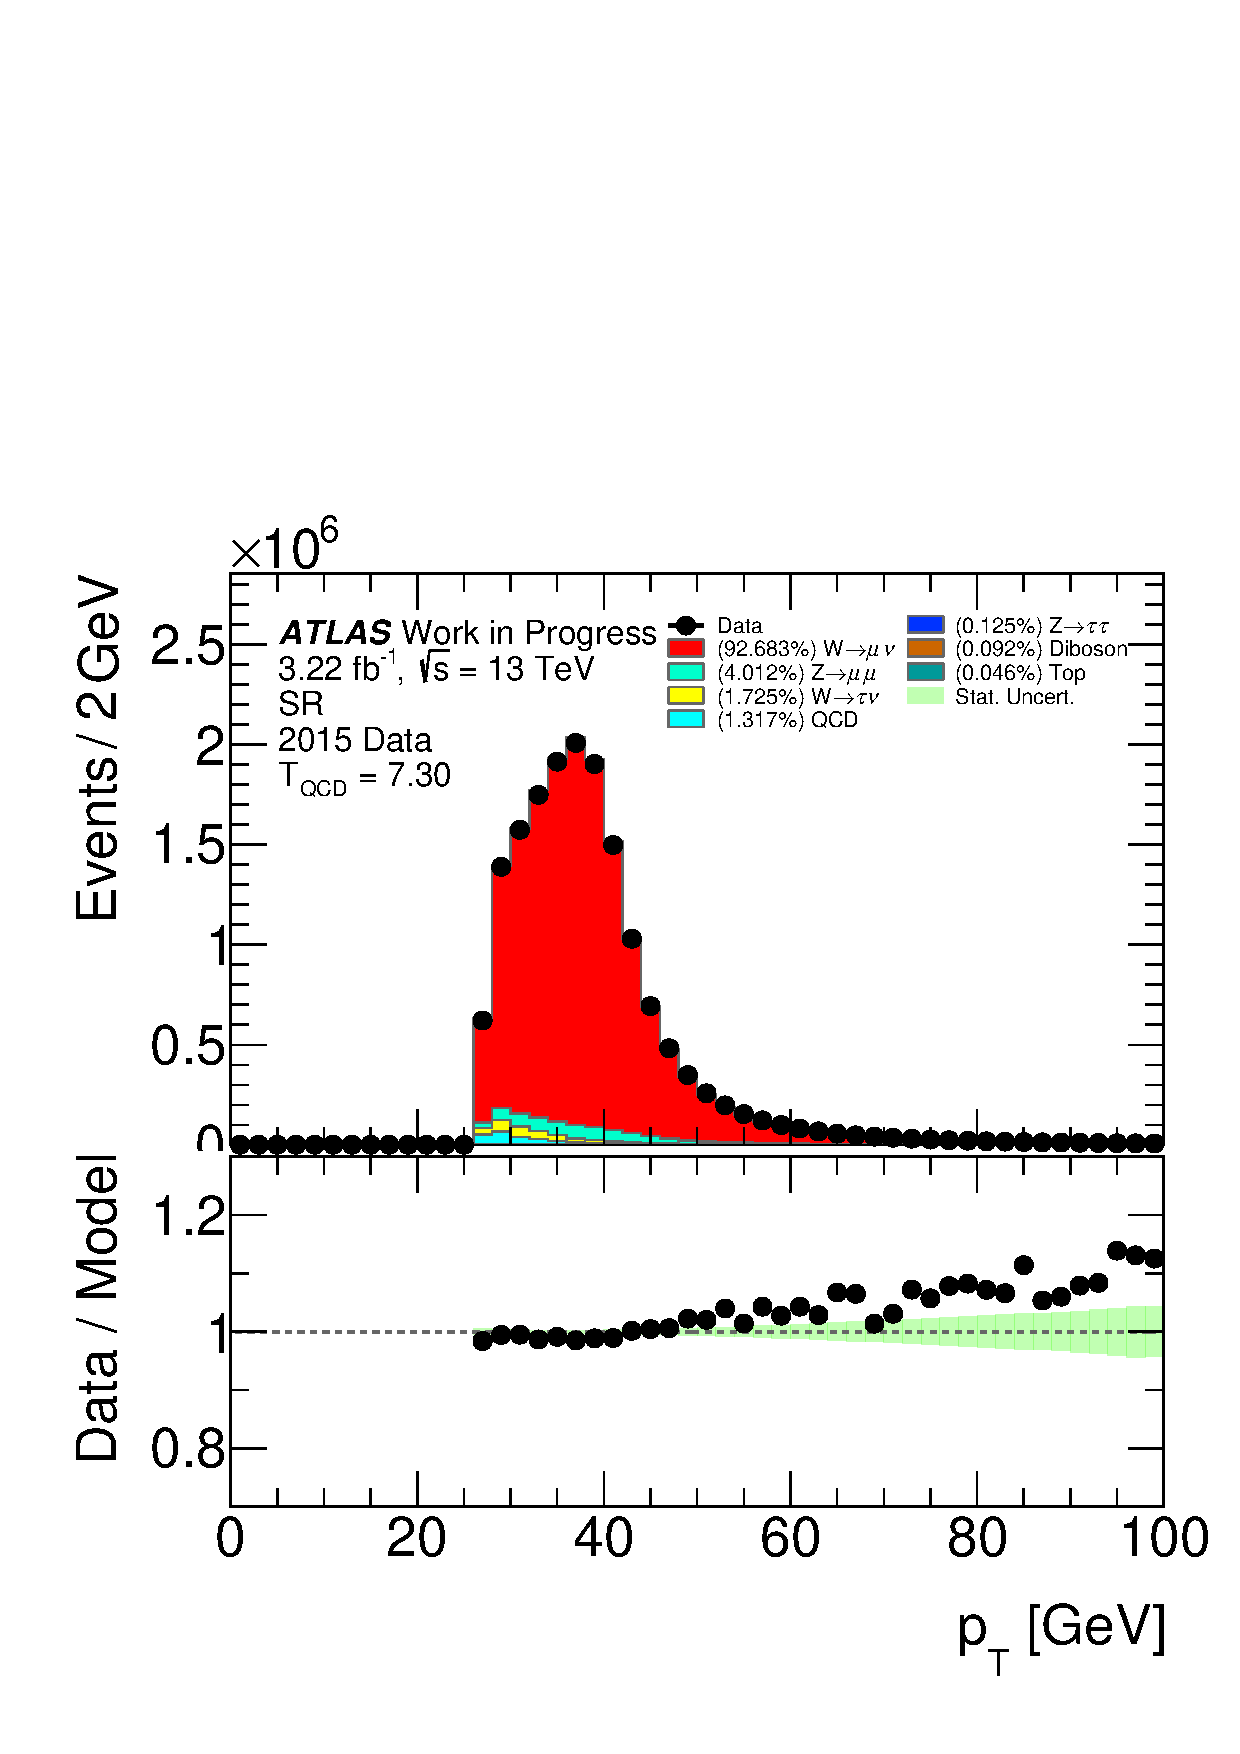
\includegraphics[width=0.45\textwidth]{figures/SR/dataMc-lep_0_pt-SR-bkgQCD-mu.pdf}
\caption{
Lepton transverse momentum distribution from the $W \rightarrow e\nu$ selection (left) and the $W \rightarrow \mu\nu$ selection (right). 
The expected contributions from all backgrounds are estimated with Monte Carlo simulations, except for the multijet background which is estimated with a data-driven method. 
% Systematic uncertainties for the signal and background distributions are combined in the shaded band, and 
Statistical uncertainties are shown on the data points.
Luminosity uncertainties are not included.
}
\label{fig:SR_lep_0_pt}
\end{figure}

\begin{figure}[htbp]
\centering
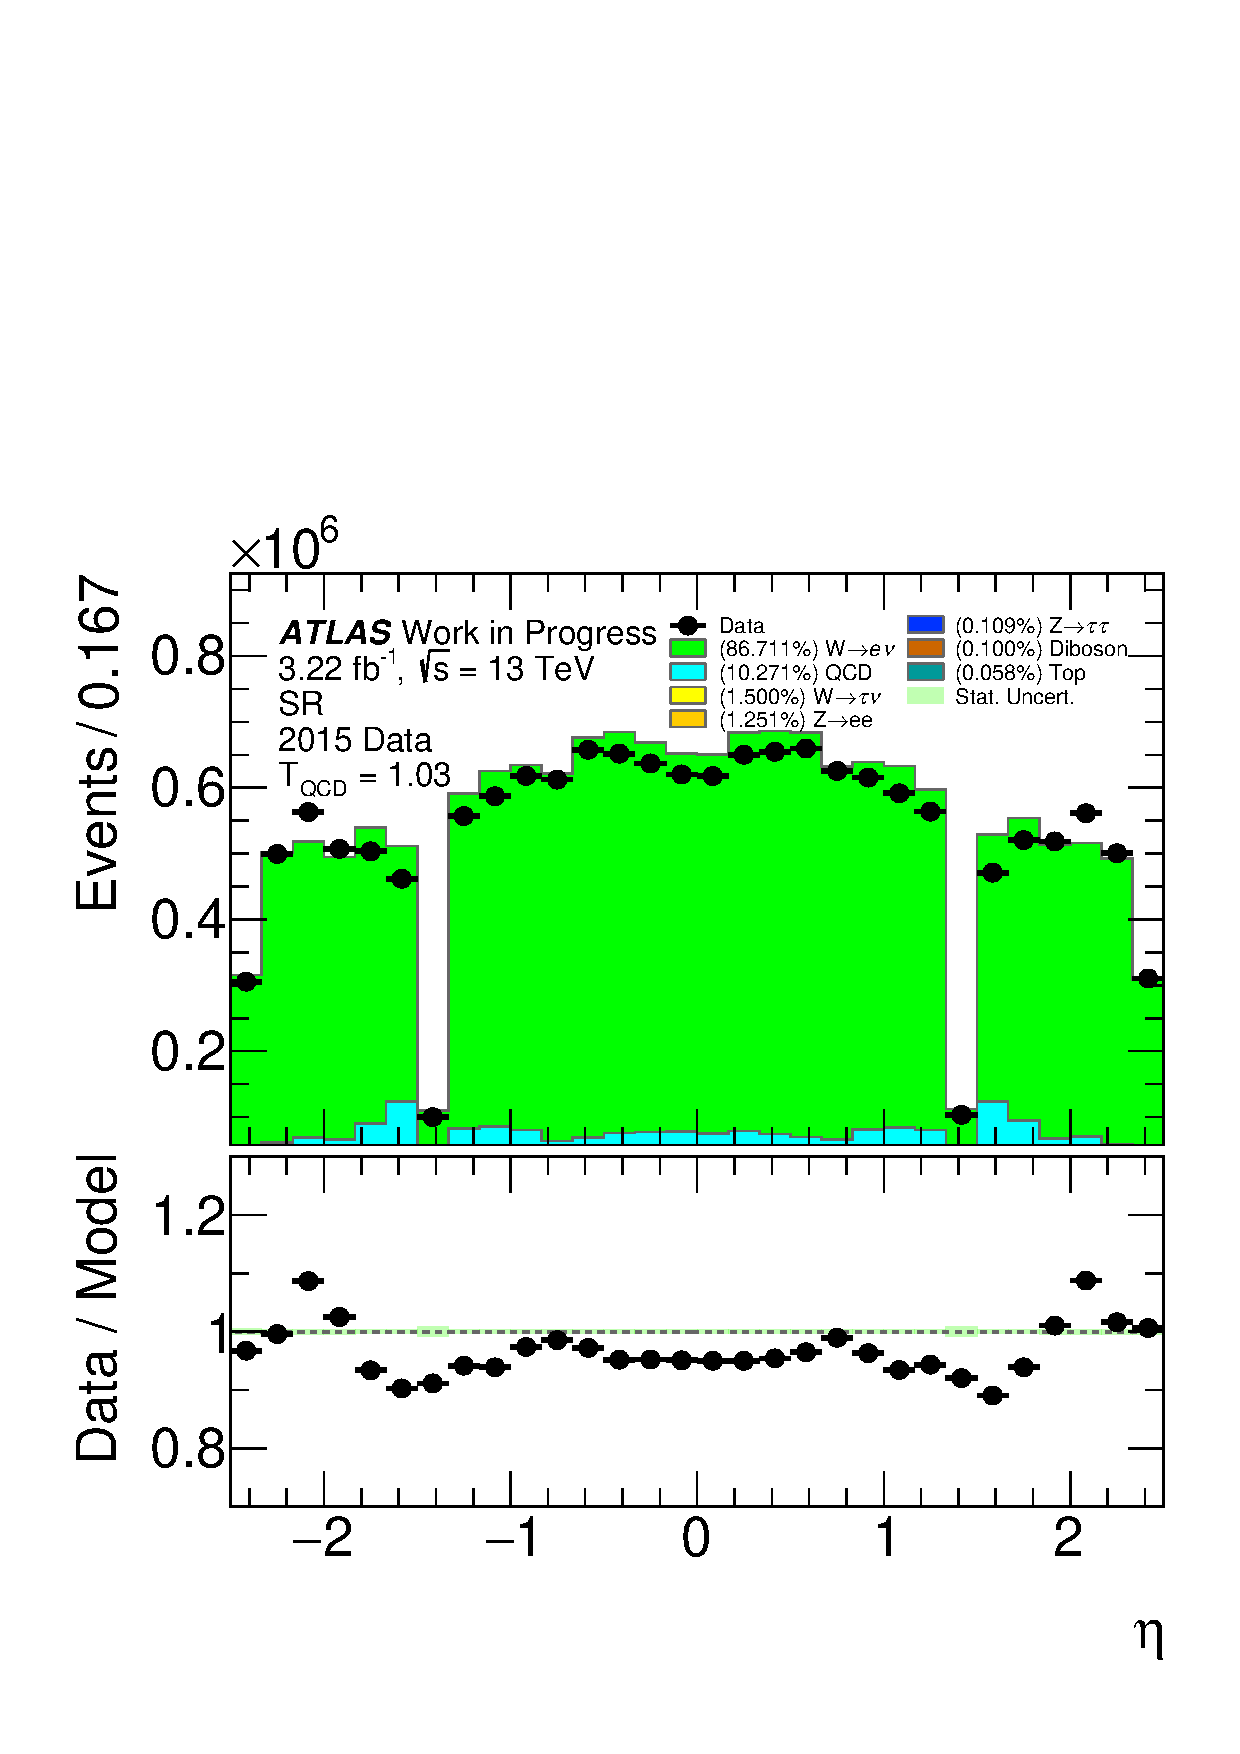
\includegraphics[width=0.45\textwidth]{figures/SR/dataMc-lep_0_eta-SR-bkgQCD-el.pdf}
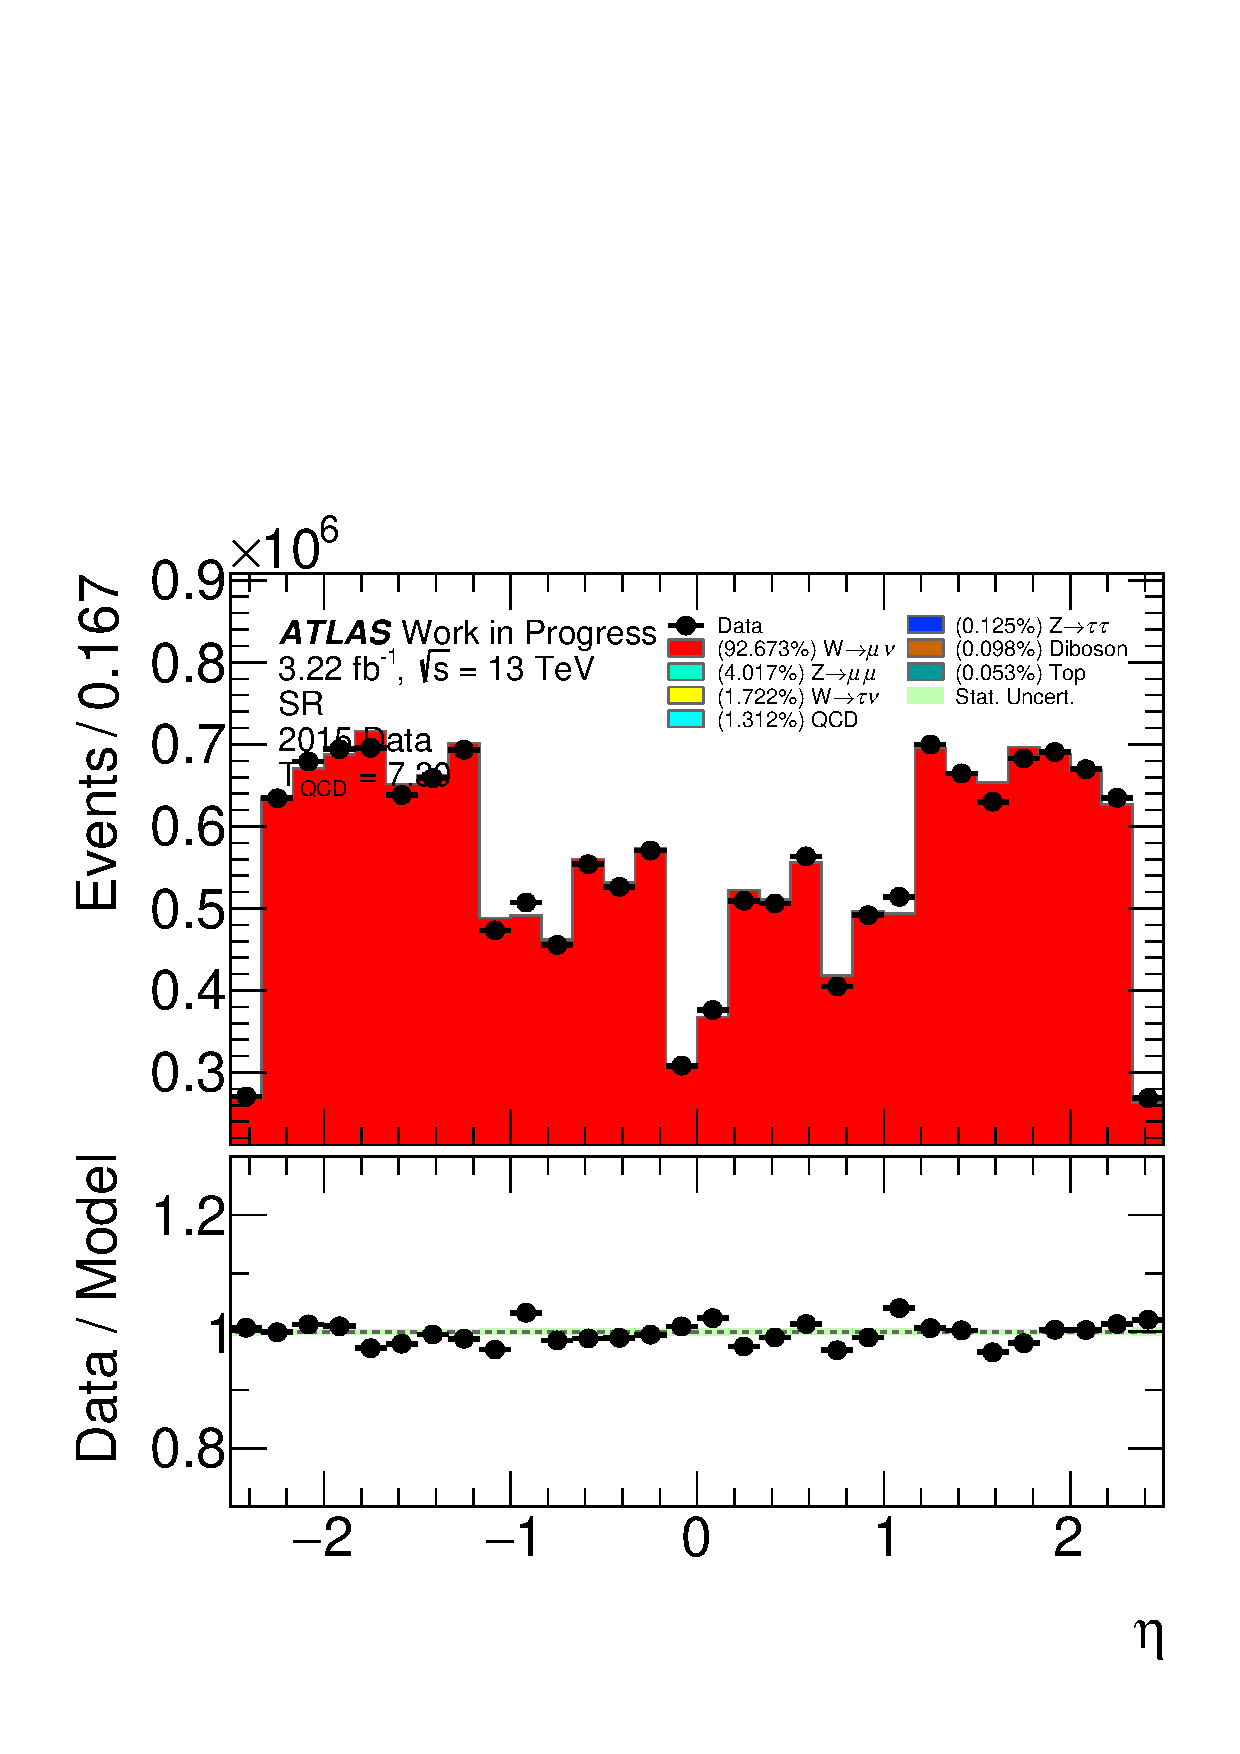
\includegraphics[width=0.45\textwidth]{figures/SR/dataMc-lep_0_eta-SR-bkgQCD-mu.pdf}
\caption{
Lepton  pseudorapidity distribution from the $W \rightarrow e\nu$ selection (left) and the $W \rightarrow \mu\nu$ selection (right). 
The expected contributions from all backgrounds are estimated with Monte Carlo simulations, except for the multijet background which is estimated with a data-driven method. 
% Systematic uncertainties for the signal and background distributions are combined in the shaded band, and 
Statistical uncertainties are shown on the data points.
Luminosity uncertainties are not included.
}
\label{fig:SR_lep_0_eta}
\end{figure}

\begin{figure}[htbp]
\centering
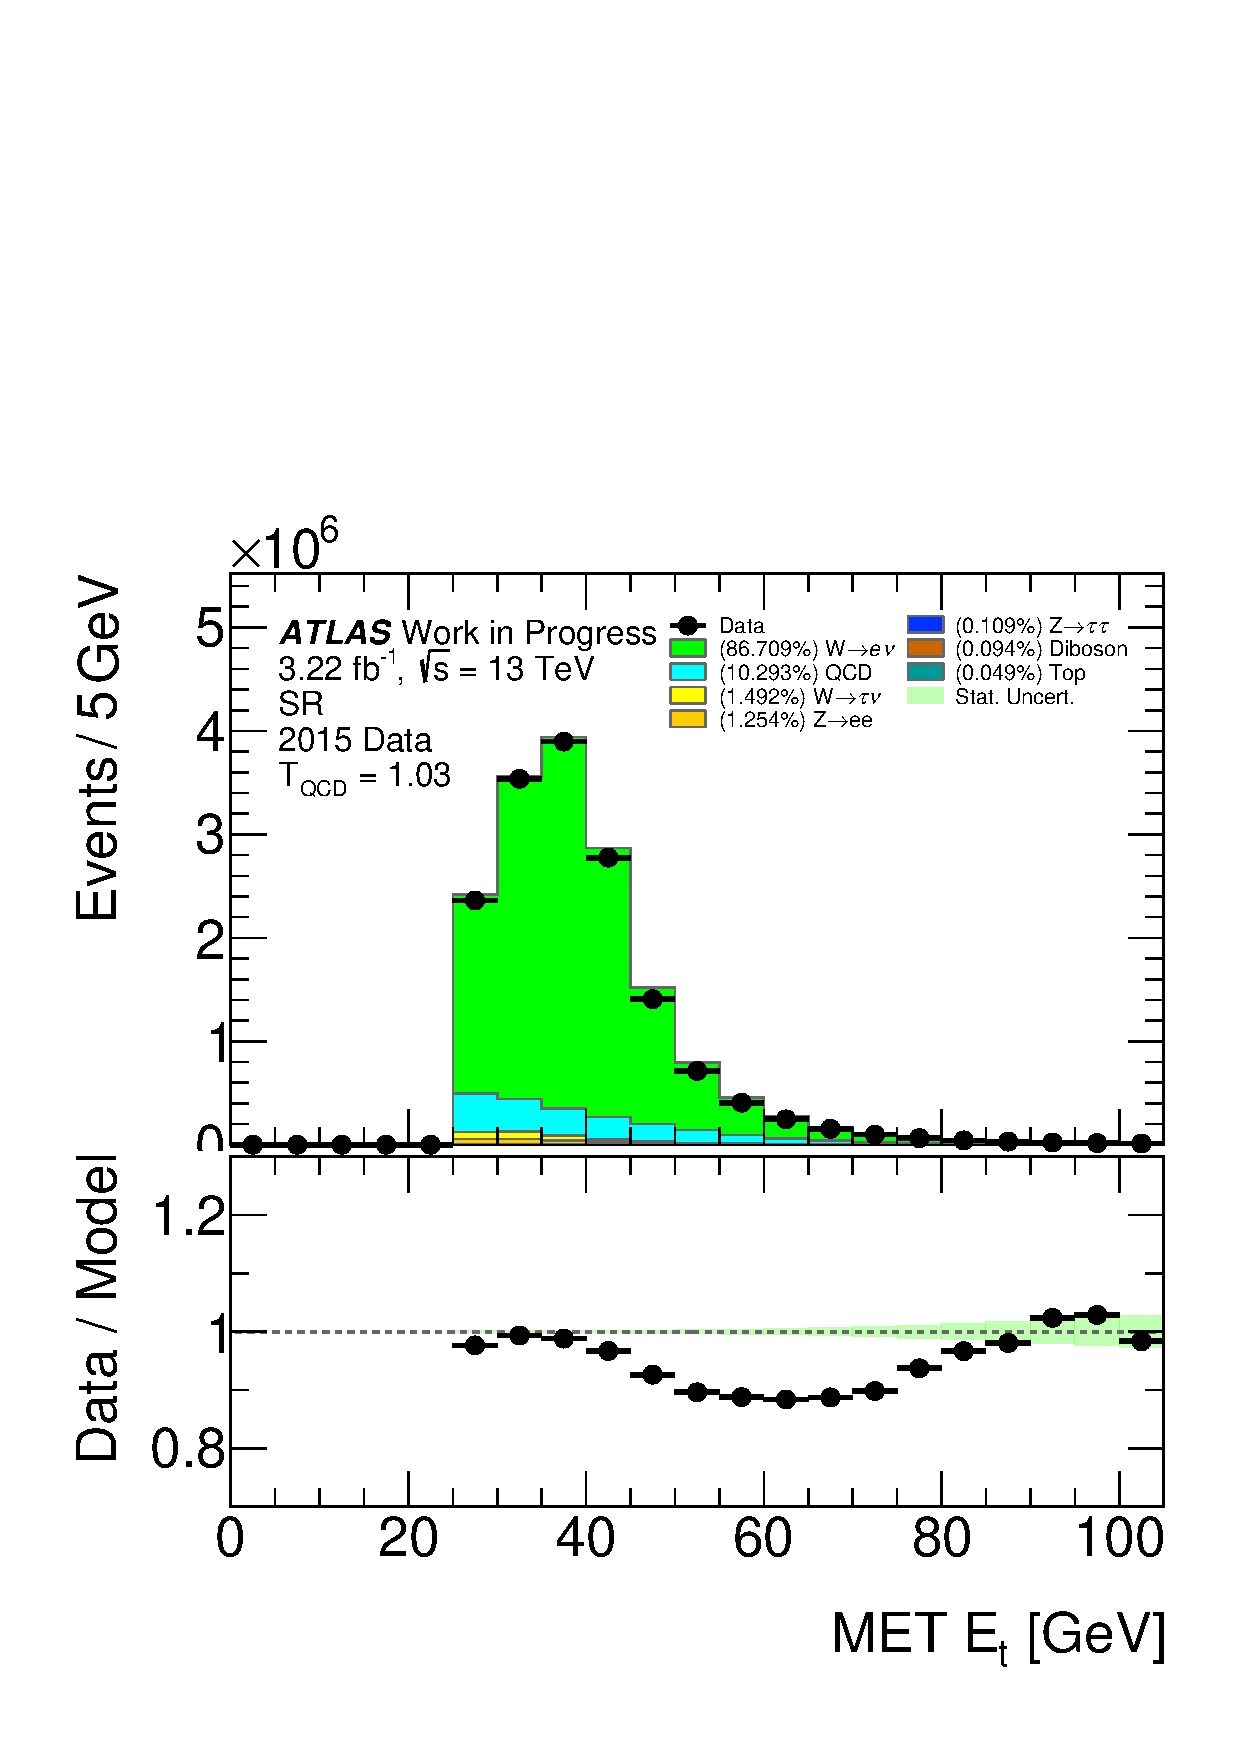
\includegraphics[width=0.45\textwidth]{figures/SR/dataMc-met_reco_et-SR-bkgQCD-el.pdf}
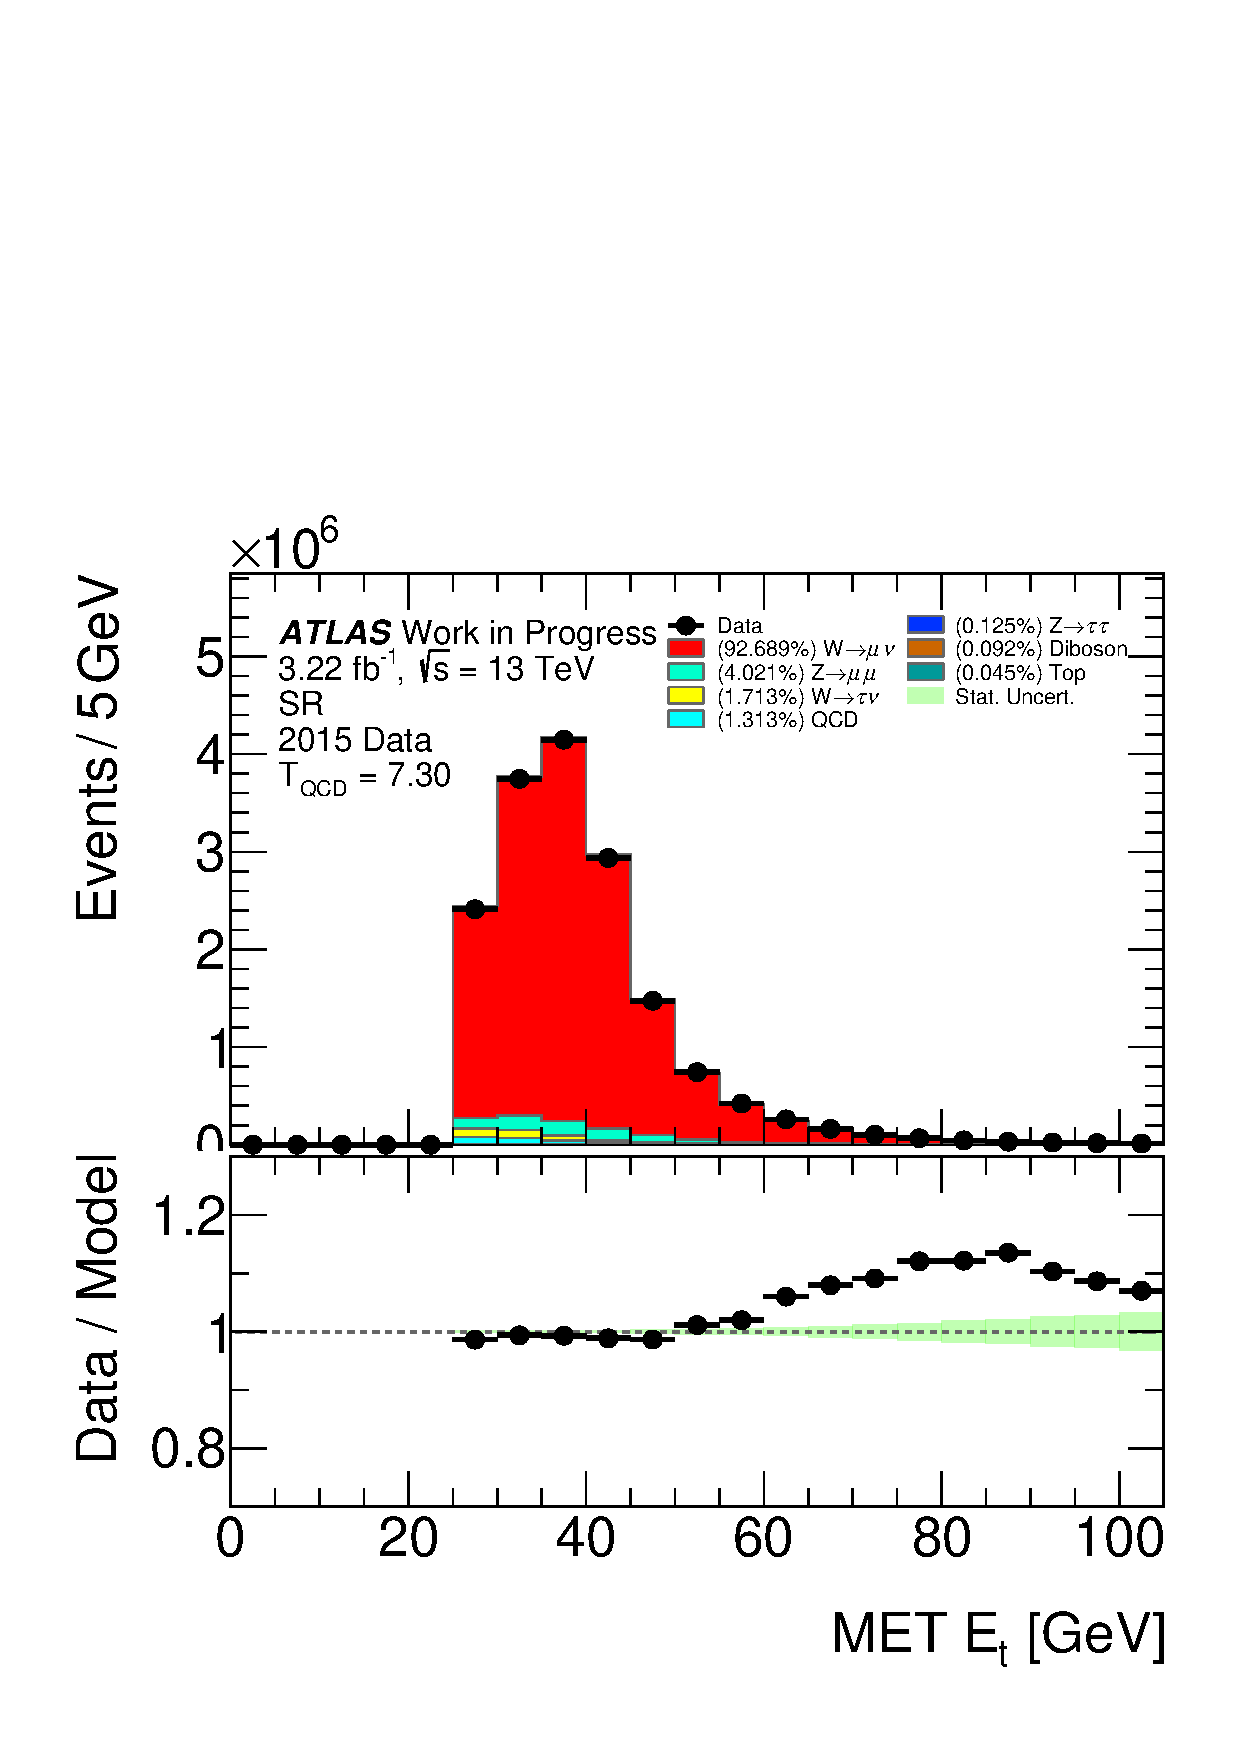
\includegraphics[width=0.45\textwidth]{figures/SR/dataMc-met_reco_et-SR-bkgQCD-mu.pdf}
\caption{
Missing transverse energy distribution from the $W \rightarrow e\nu$ selection (left) and the $W \rightarrow \mu\nu$ selection (right).
The $E_{T}^{miss}$ has been recalibrated using the best energy calibration for each of the identified physics objects.
The expected contributions from all backgrounds are estimated with Monte Carlo simulations, except for the multijet background which is estimated with a data-driven method. 
% Systematic uncertainties for the signal and background distributions are combined in the shaded band, and 
Statistical uncertainties are shown on the data points.
Luminosity uncertainties are not included.
}
\label{fig:SR_met_reco_et}
\end{figure}

\begin{figure}[htbp]
\centering
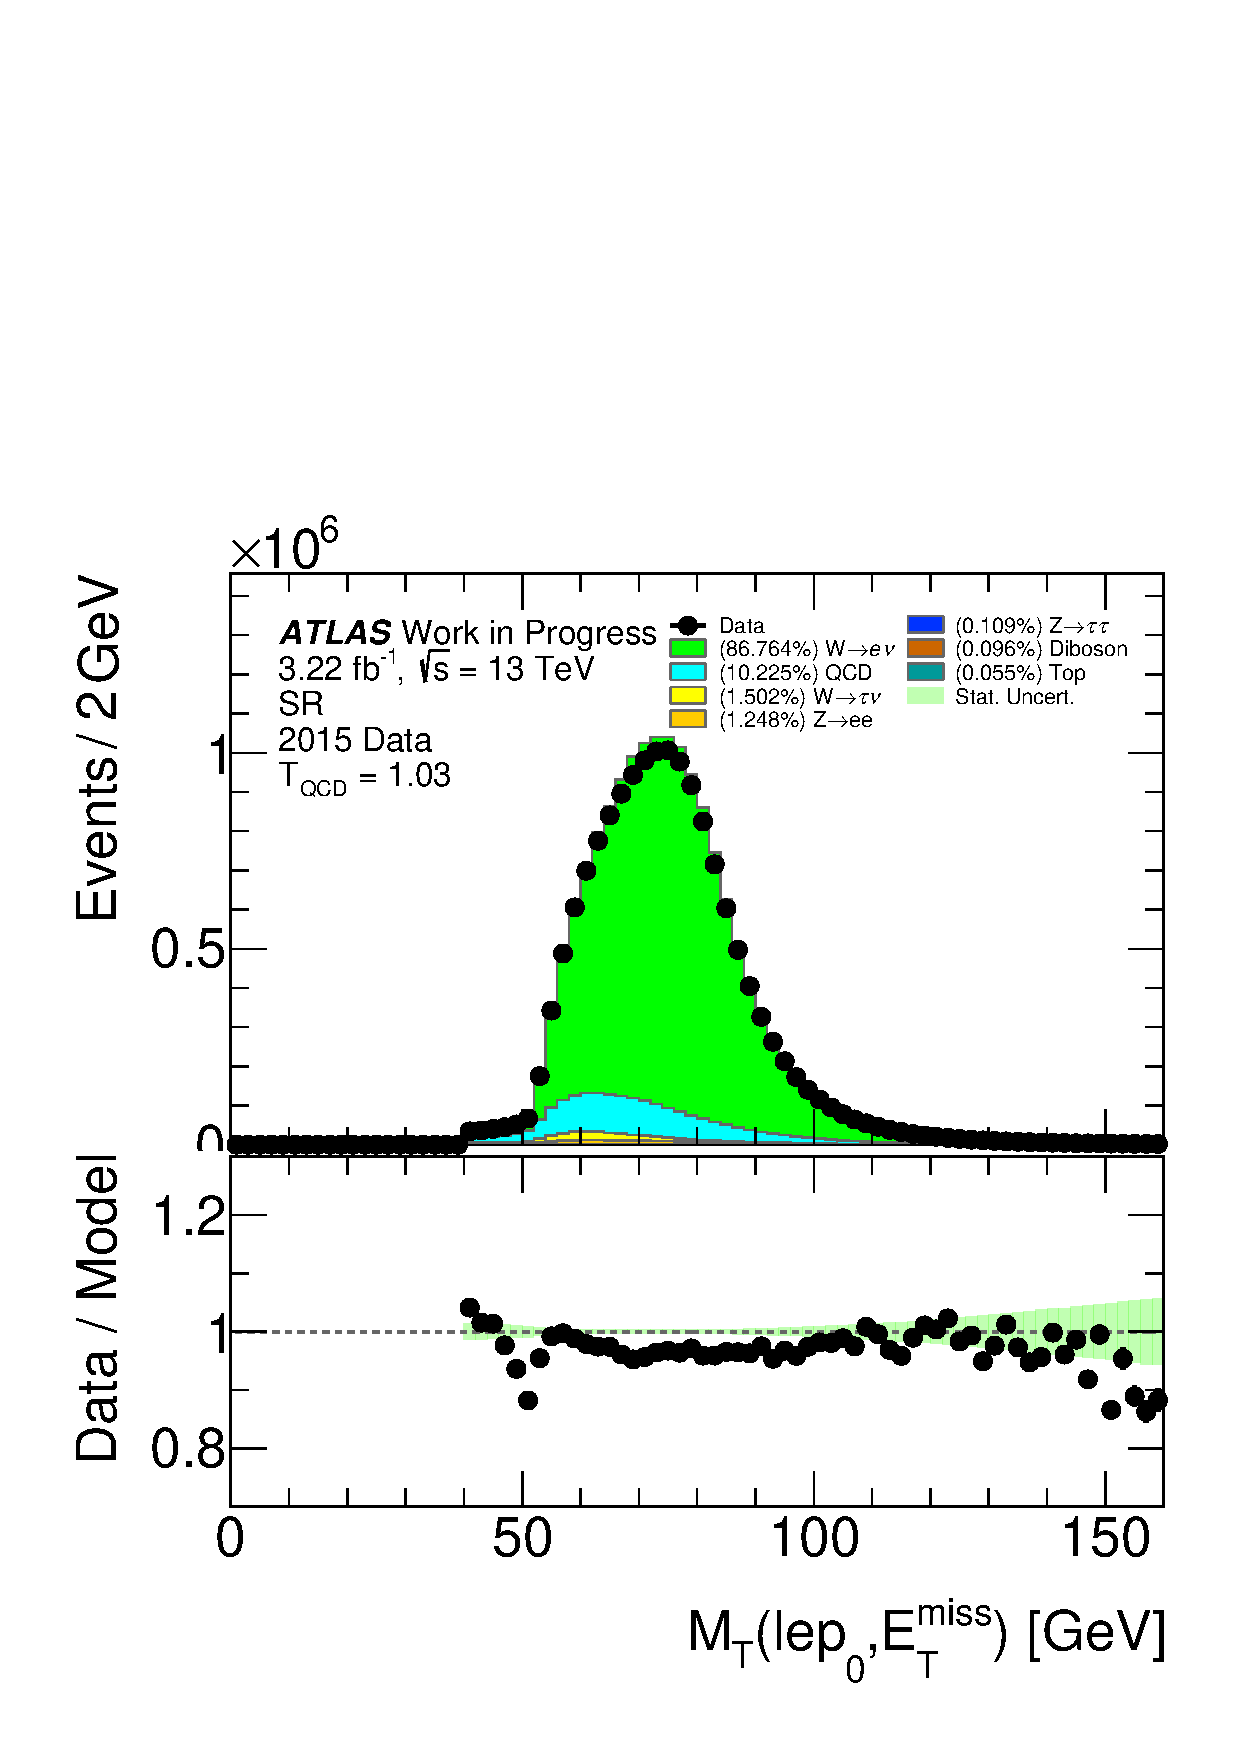
\includegraphics[width=0.45\textwidth]{figures/SR/dataMc-lepmet_mt-SR-bkgQCD-el.pdf}
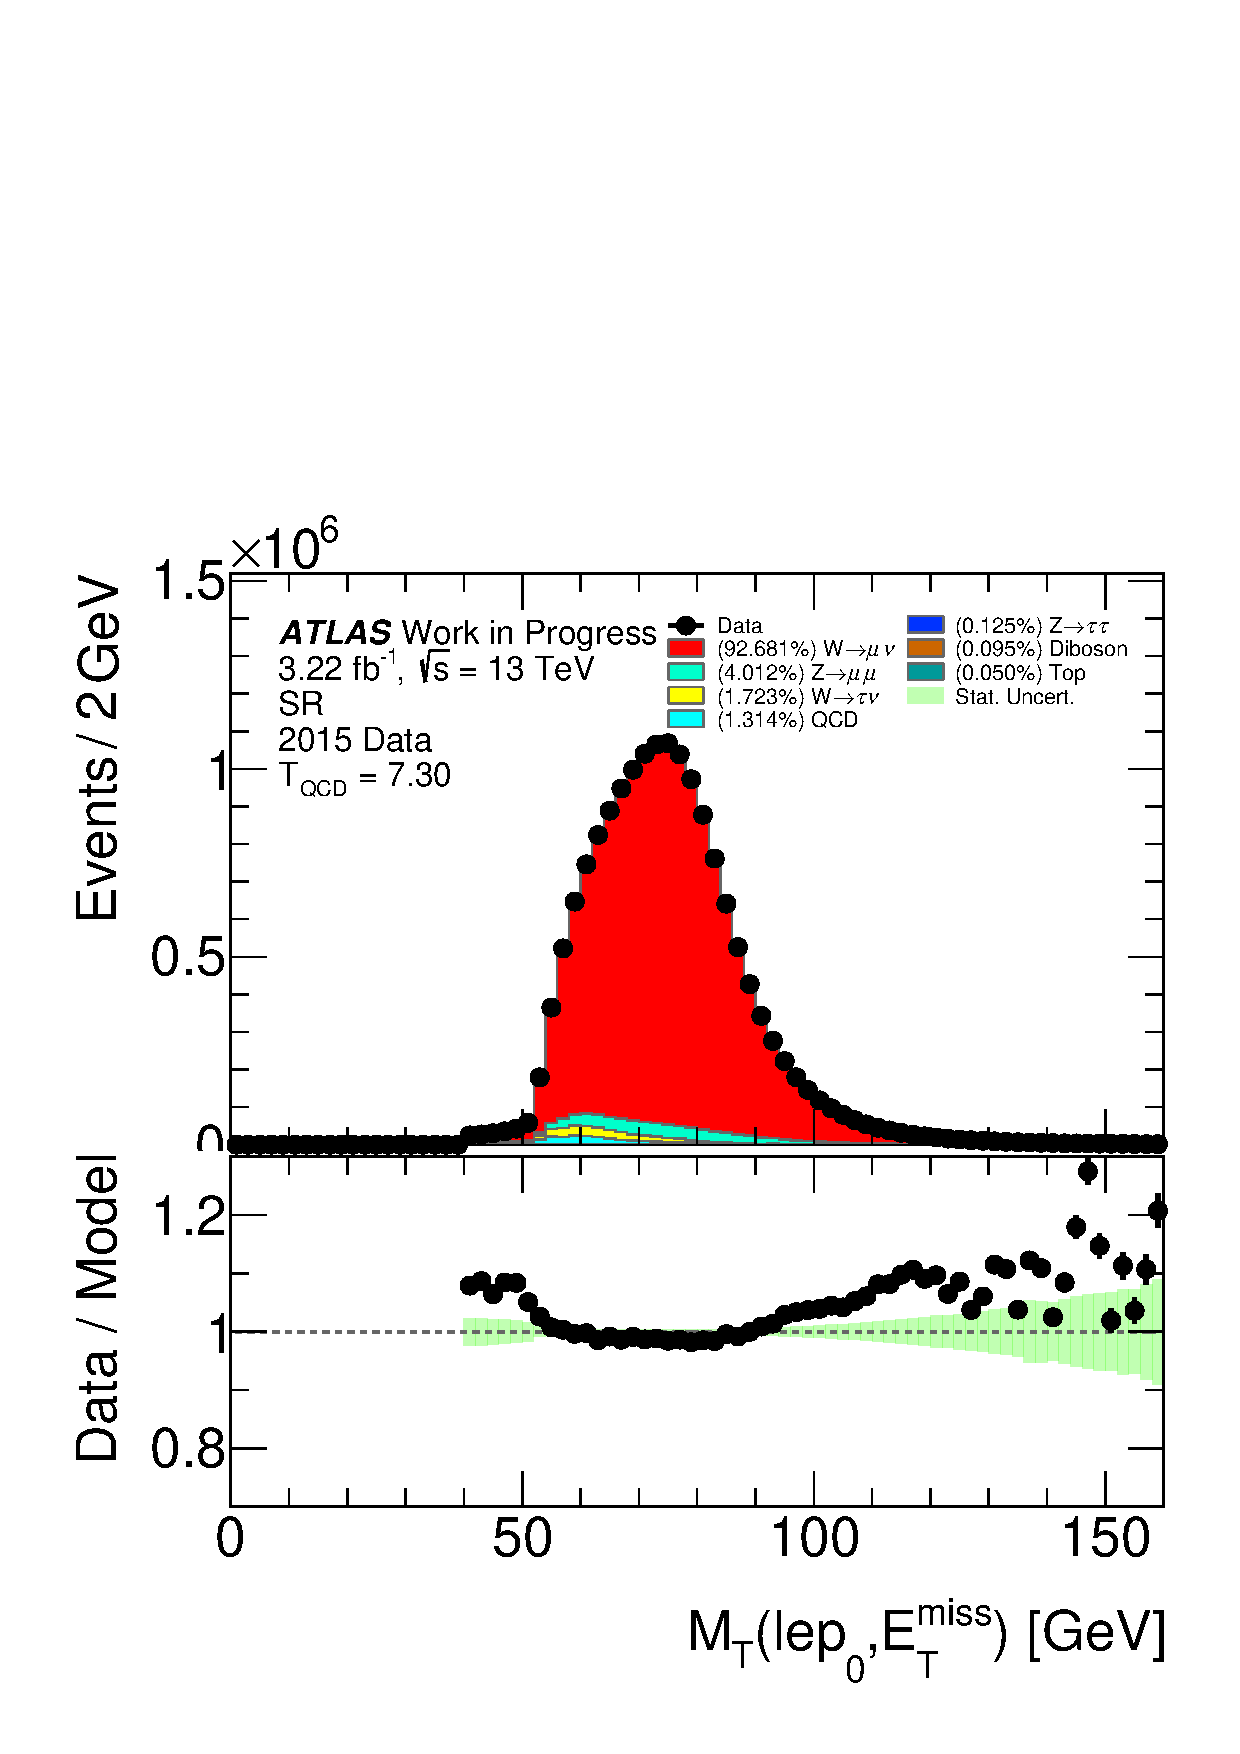
\includegraphics[width=0.45\textwidth]{figures/SR/dataMc-lepmet_mt-SR-bkgQCD-mu.pdf}
\caption{
Transverse mass distribution, calculated from the lepton and the $E_{T}^{miss}$ from the $W \rightarrow e\nu$ selection (left) and the $W \rightarrow \mu\nu$ selection (right).
The $E_{T}^{miss}$ has been recalibrated using the best energy calibration for each of the identified physics objects.
The expected contributions from all backgrounds are estimated with Monte Carlo simulations, except for the multijet background which is estimated with a data-driven method. 
% Systematic uncertainties for the signal and background distributions are combined in the shaded band, and 
Statistical uncertainties are shown on the data points.
Luminosity uncertainties are not included.
}
\label{fig:SR_met_reco_et}
\end{figure}

\begin{figure}[htbp]
\centering
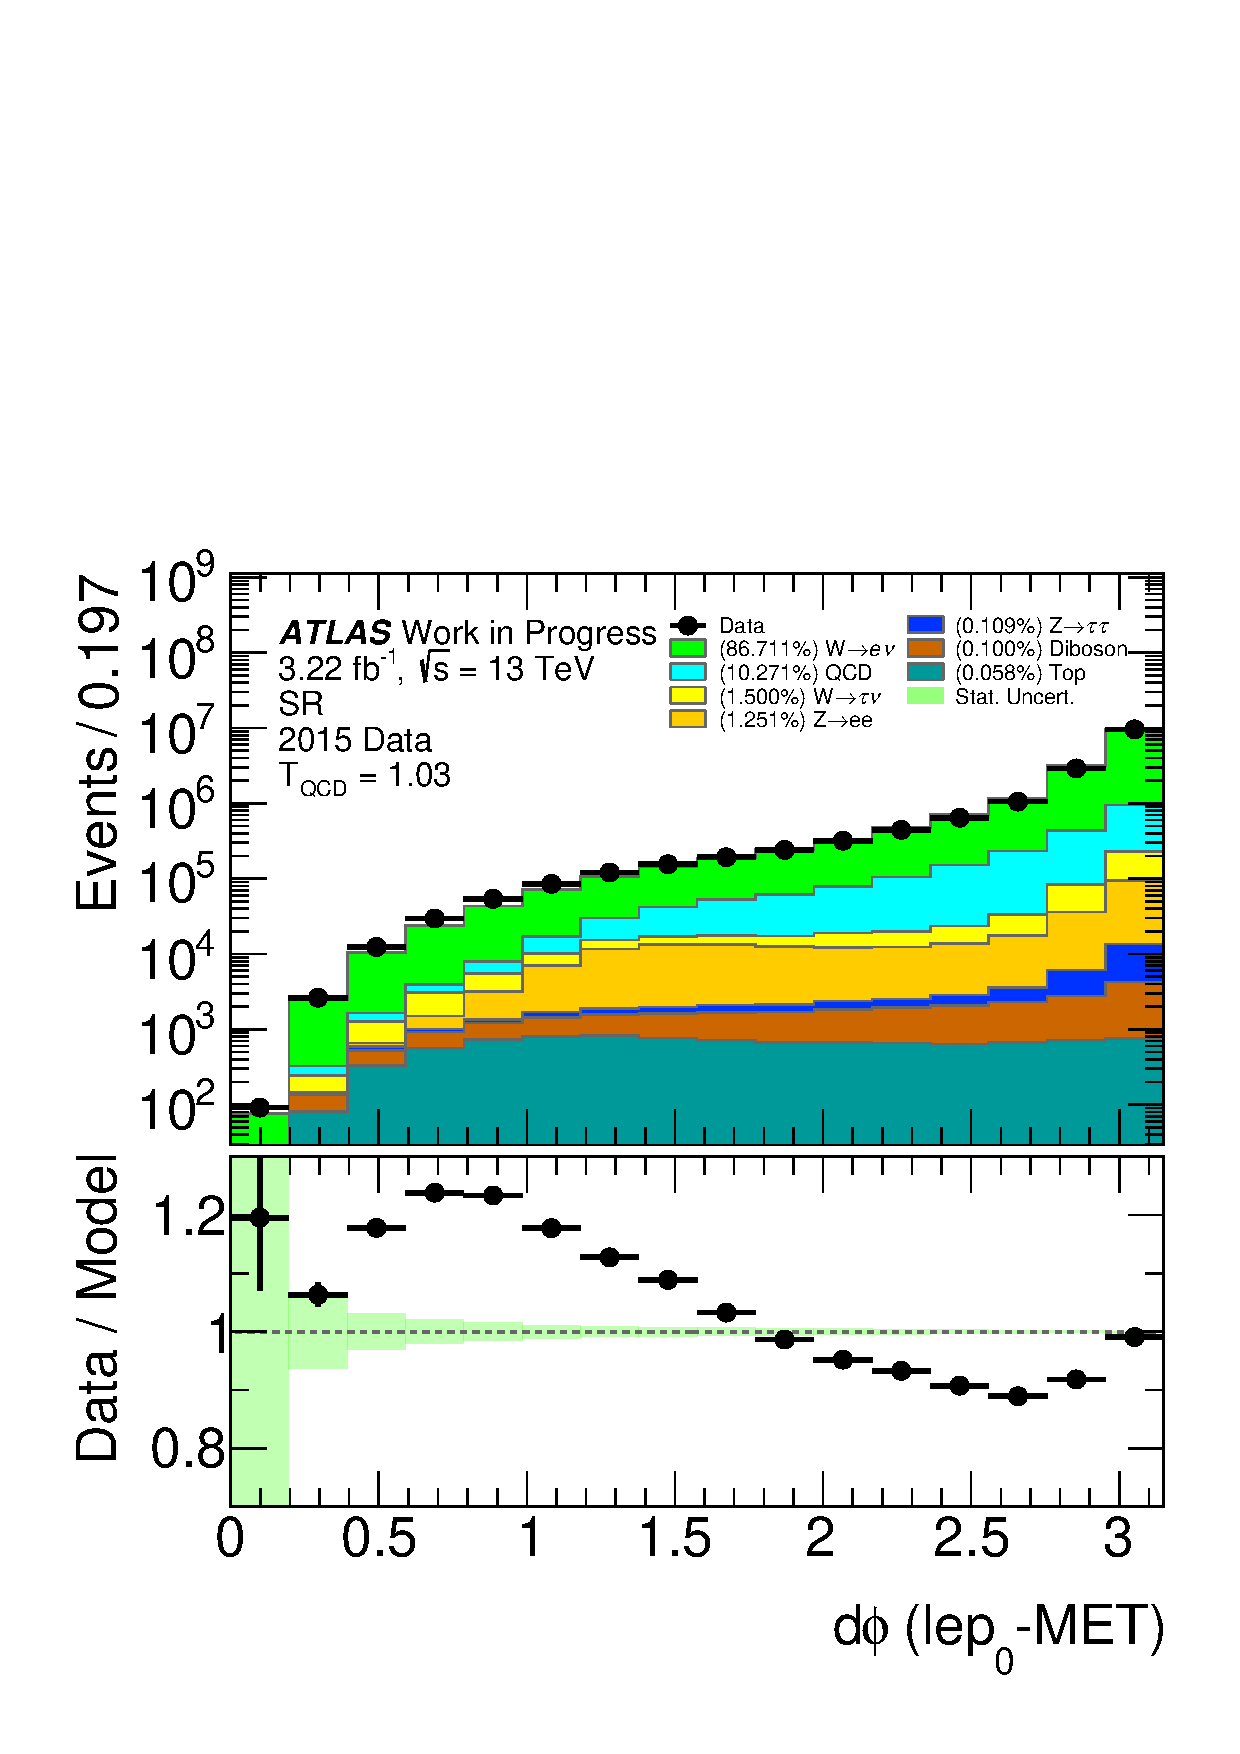
\includegraphics[width=0.45\textwidth]{figures/SR/dataMc-lepmet_dphi-SR-bkgQCD-el-log.pdf}
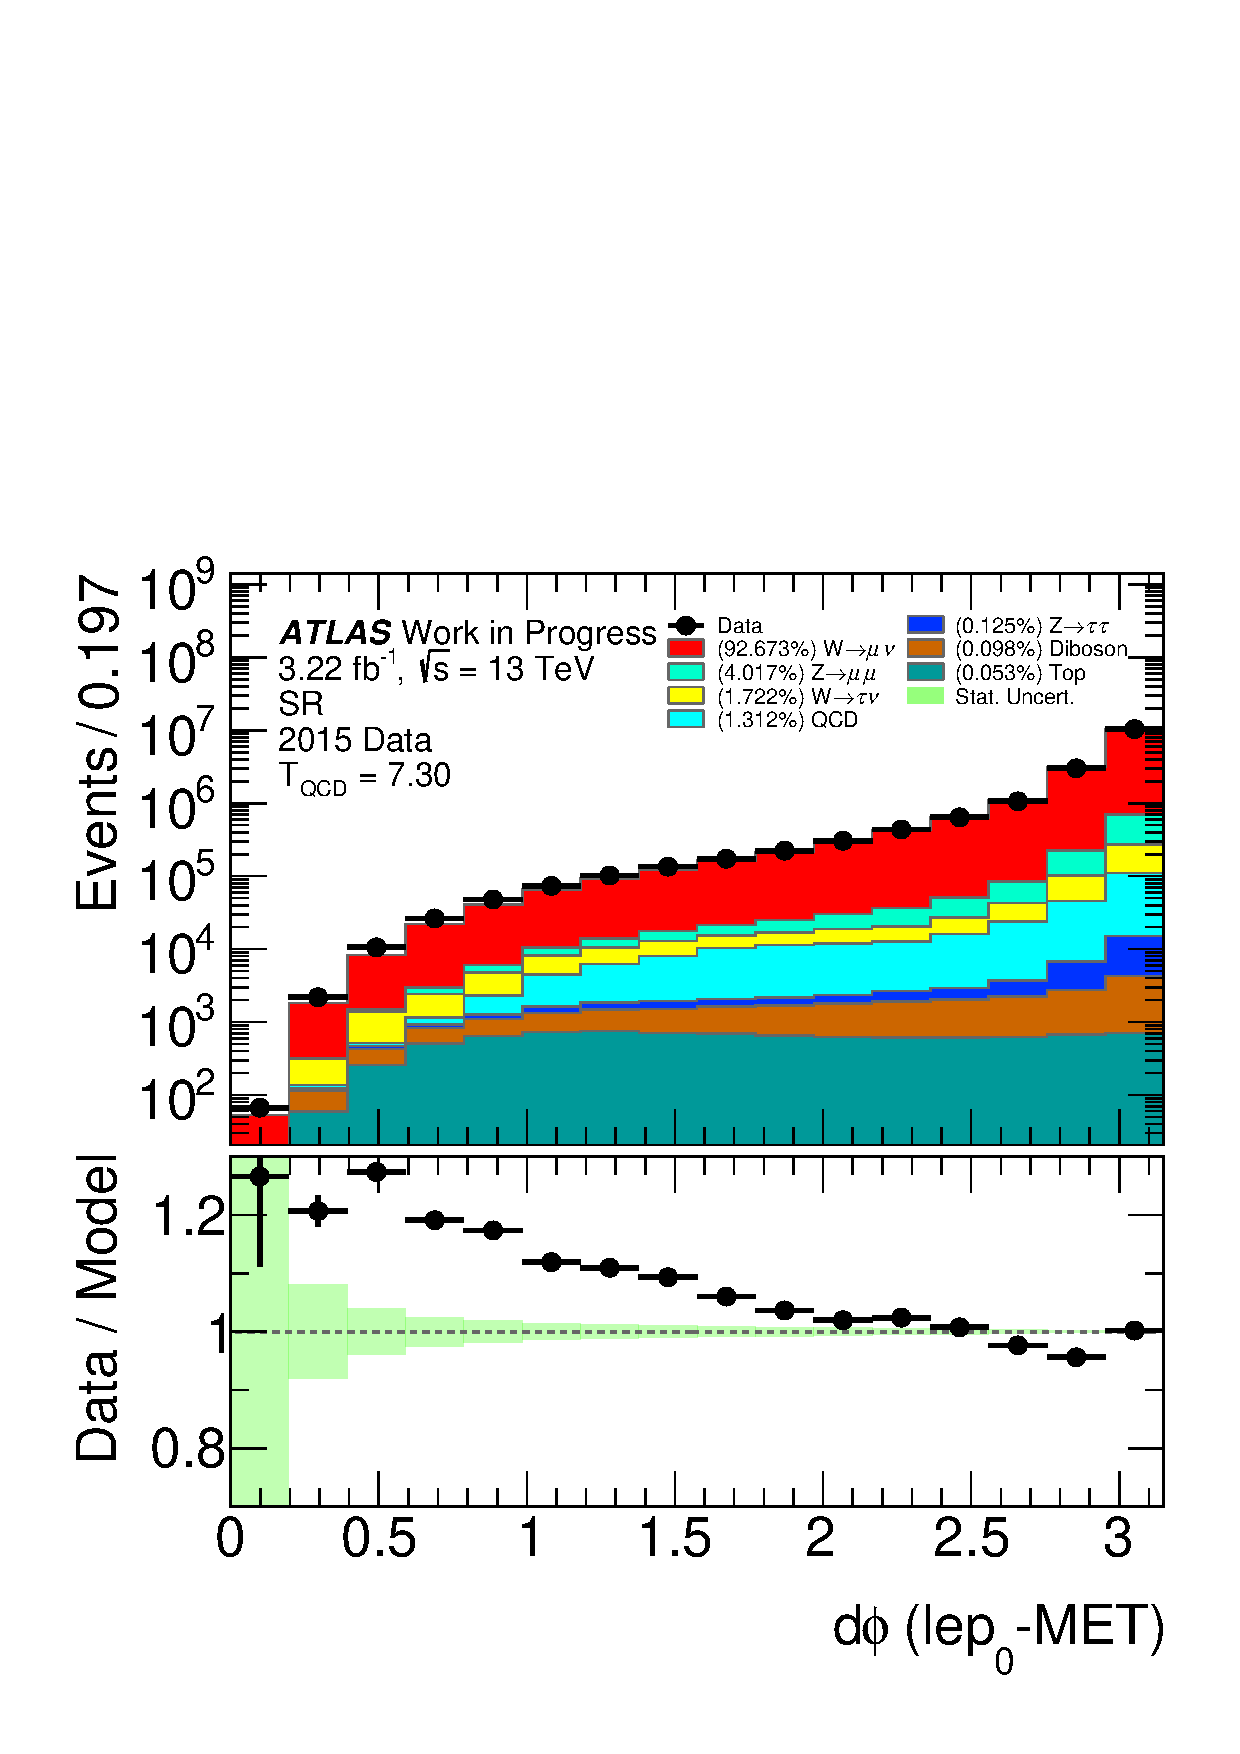
\includegraphics[width=0.45\textwidth]{figures/SR/dataMc-lepmet_dphi-SR-bkgQCD-mu-log.pdf}
\caption{
Azimuthal angle distribution, calculated as azimuthal angle difference of the leading lepton and the $E_{T}^{miss}$ from the $W \rightarrow e\nu$ selection (left) and the $W \rightarrow \mu\nu$ selection (right).
The $E_{T}^{miss}$ has been recalibrated using the best energy calibration for each of the identified physics objects.
The expected contributions from all backgrounds are estimated with Monte Carlo simulations, except for the multijet background which is estimated with a data-driven method. 
% Systematic uncertainties for the signal and background distributions are combined in the shaded band, and 
Statistical uncertainties are shown on the data points.
Luminosity uncertainties are not included.
}
\label{fig:SR_lepmet_dphi}
\end{figure}

% ##################
% ZR
% ##################

\begin{figure}[htbp]
\centering
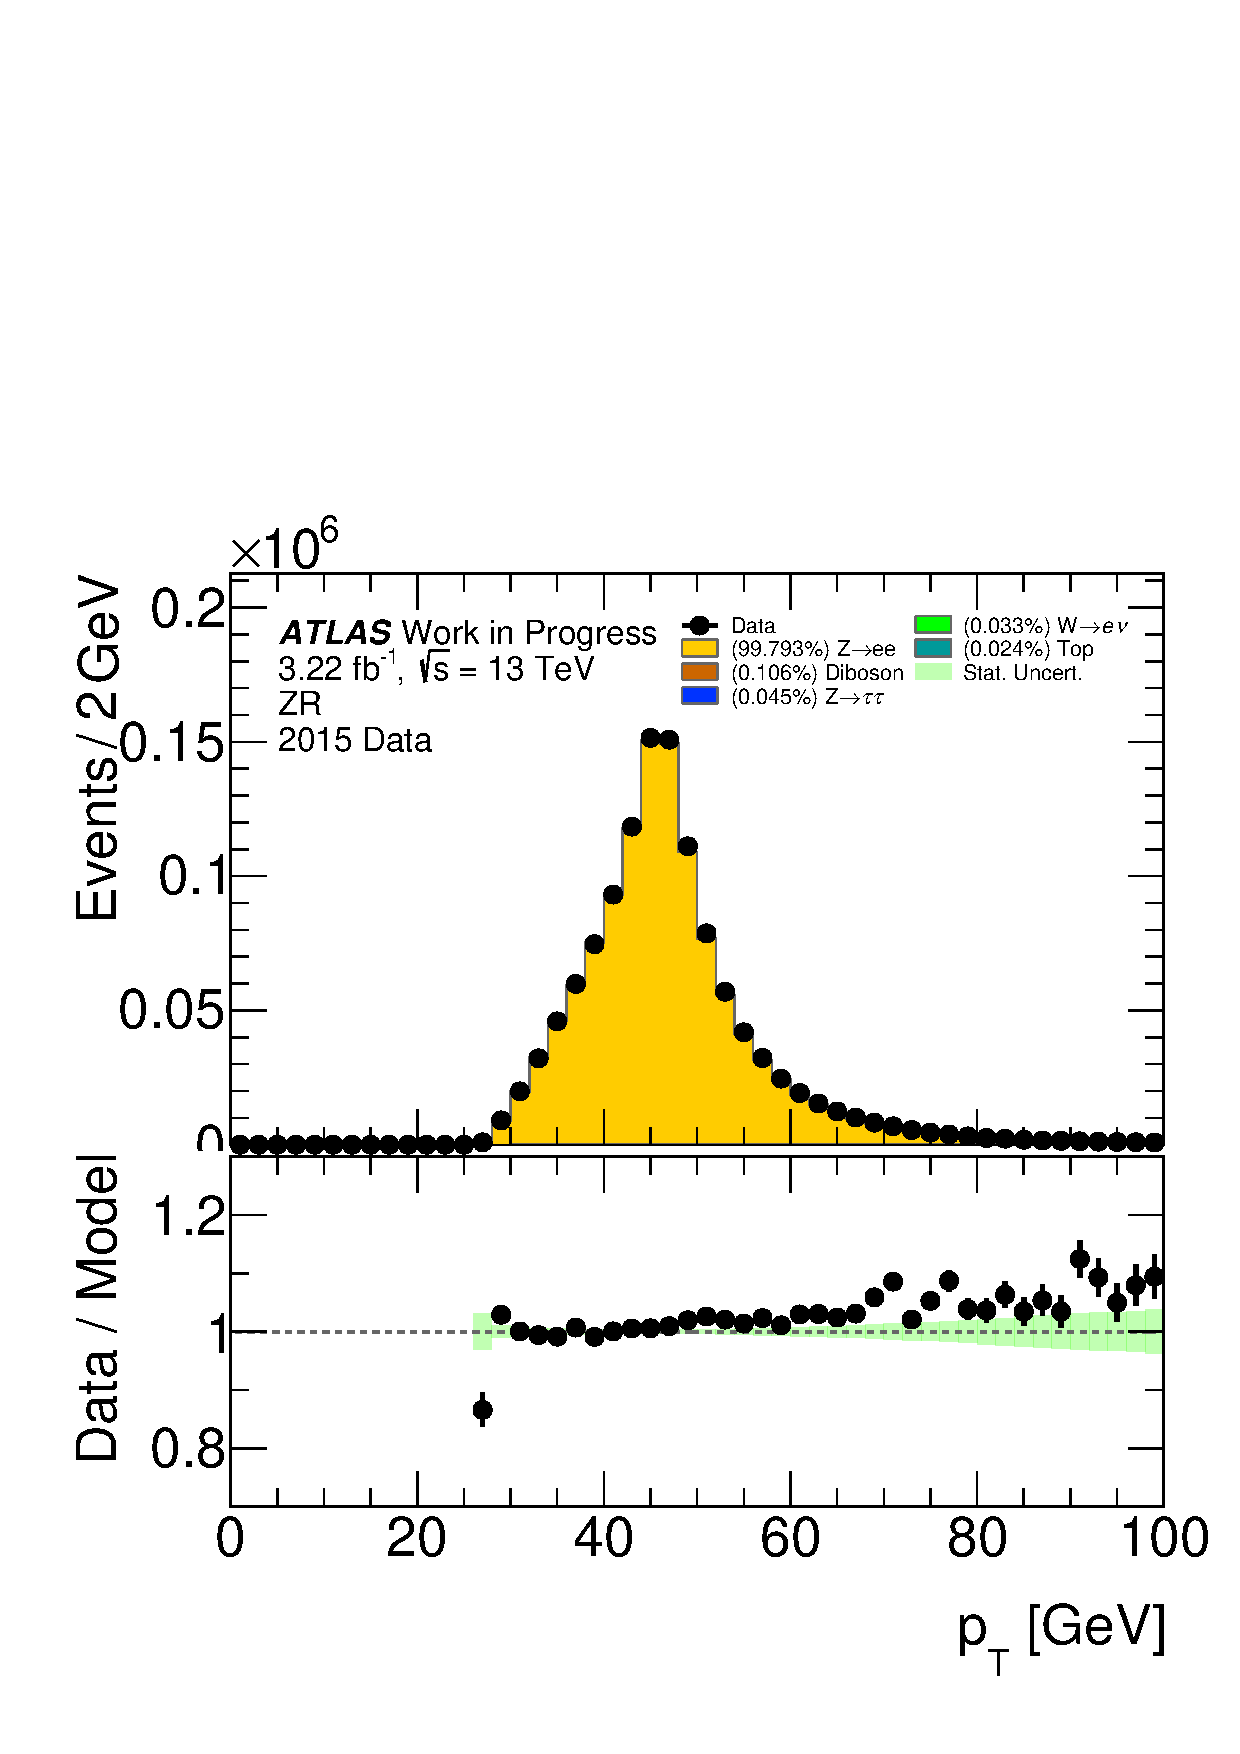
\includegraphics[width=0.45\textwidth]{figures/ZR/dataMc-lep_0_pt-ZR-el.pdf}
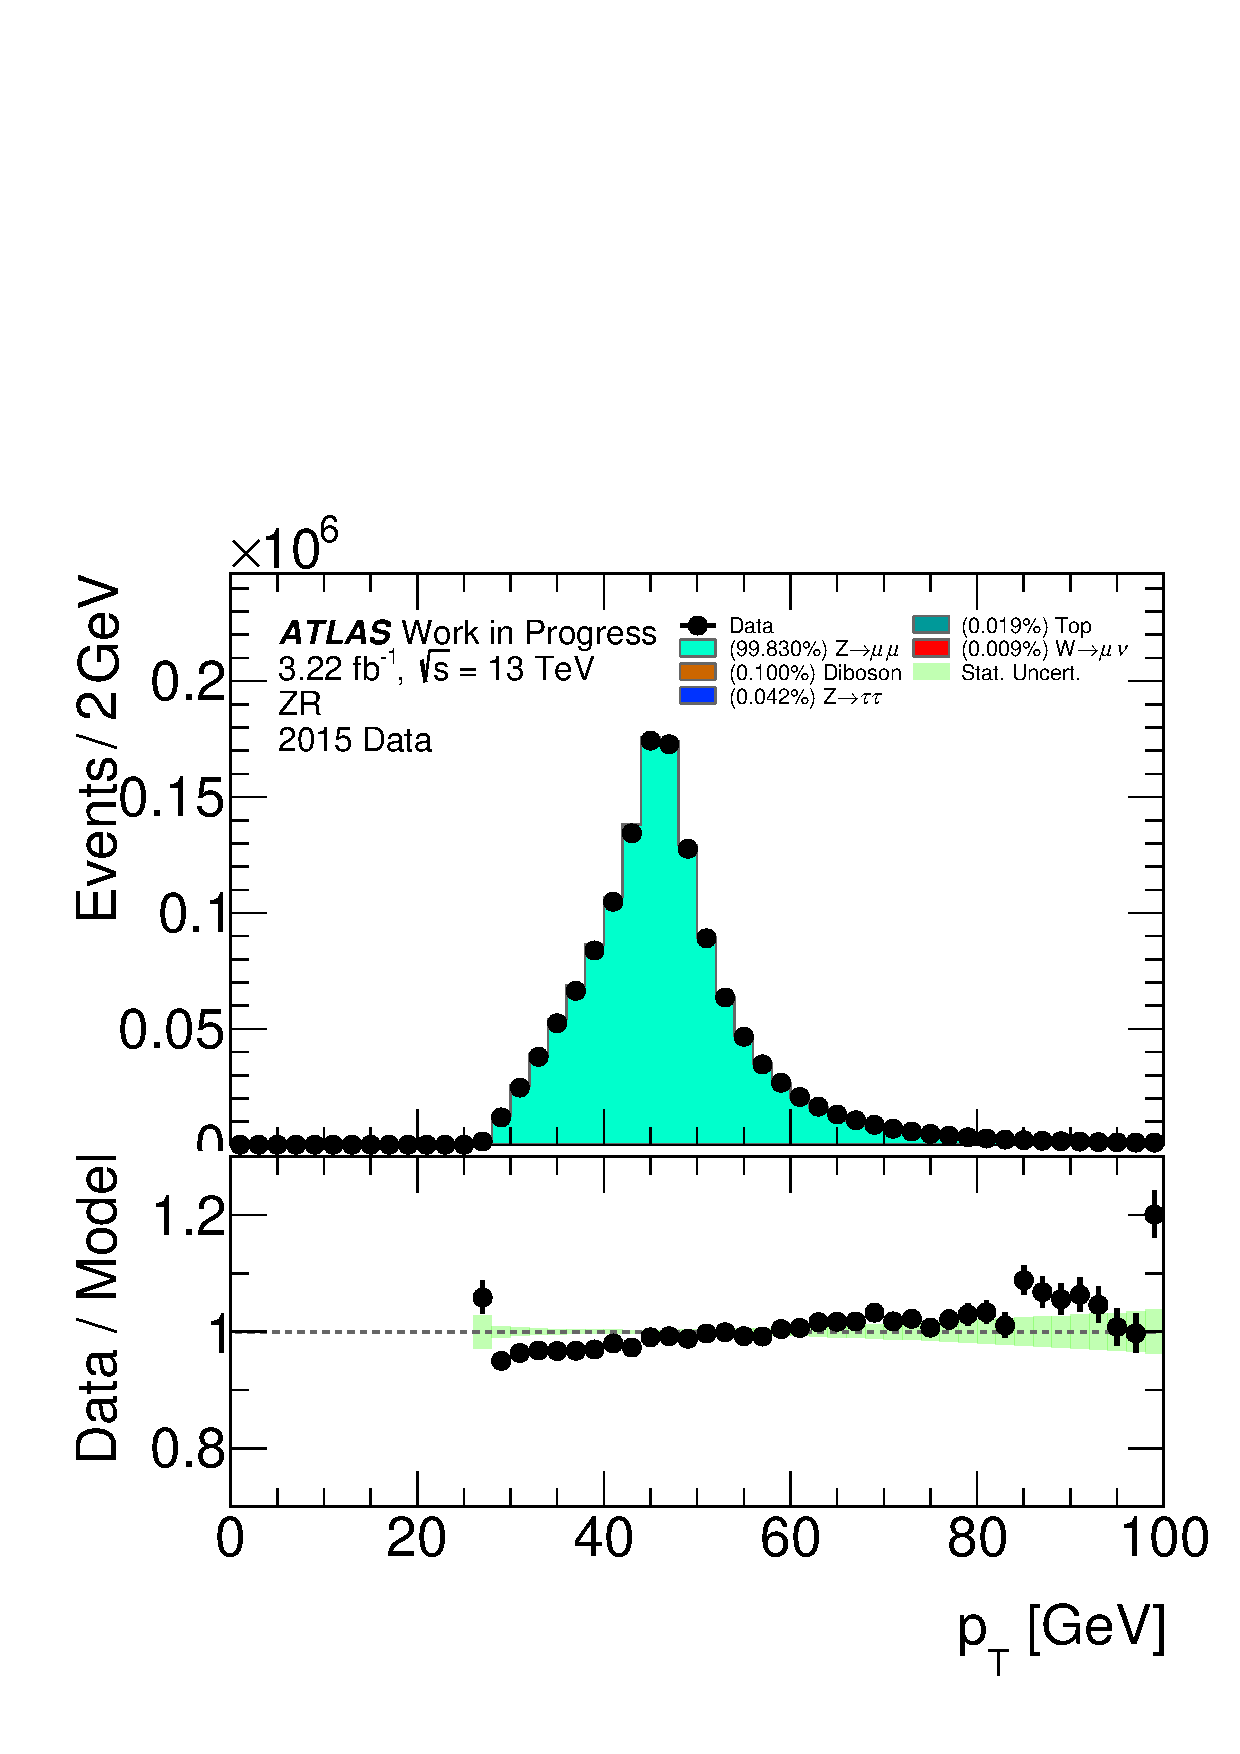
\includegraphics[width=0.45\textwidth]{figures/ZR/dataMc-lep_0_pt-ZR-mu.pdf}
\caption{
Leading lepton transverse momentum distributions from the $Z \rightarrow e^+e^-$ selection (left) and the $Z \rightarrow \mu^+\mu^-$  selection (right).
The expected contributions from all backgrounds are estimated with Monte Carlo simulations.
The background processes are heavily suppressed and not visible on the linear scale. 
% Systematic uncertainties for the signal and background distributions are combined in the shaded band, and 
Statistical uncertainties are shown on the data points.
Luminosity uncertainties are not included.
}
\label{fig:ZR_lep_0_pt}
\end{figure}

\begin{figure}[htbp]
\centering
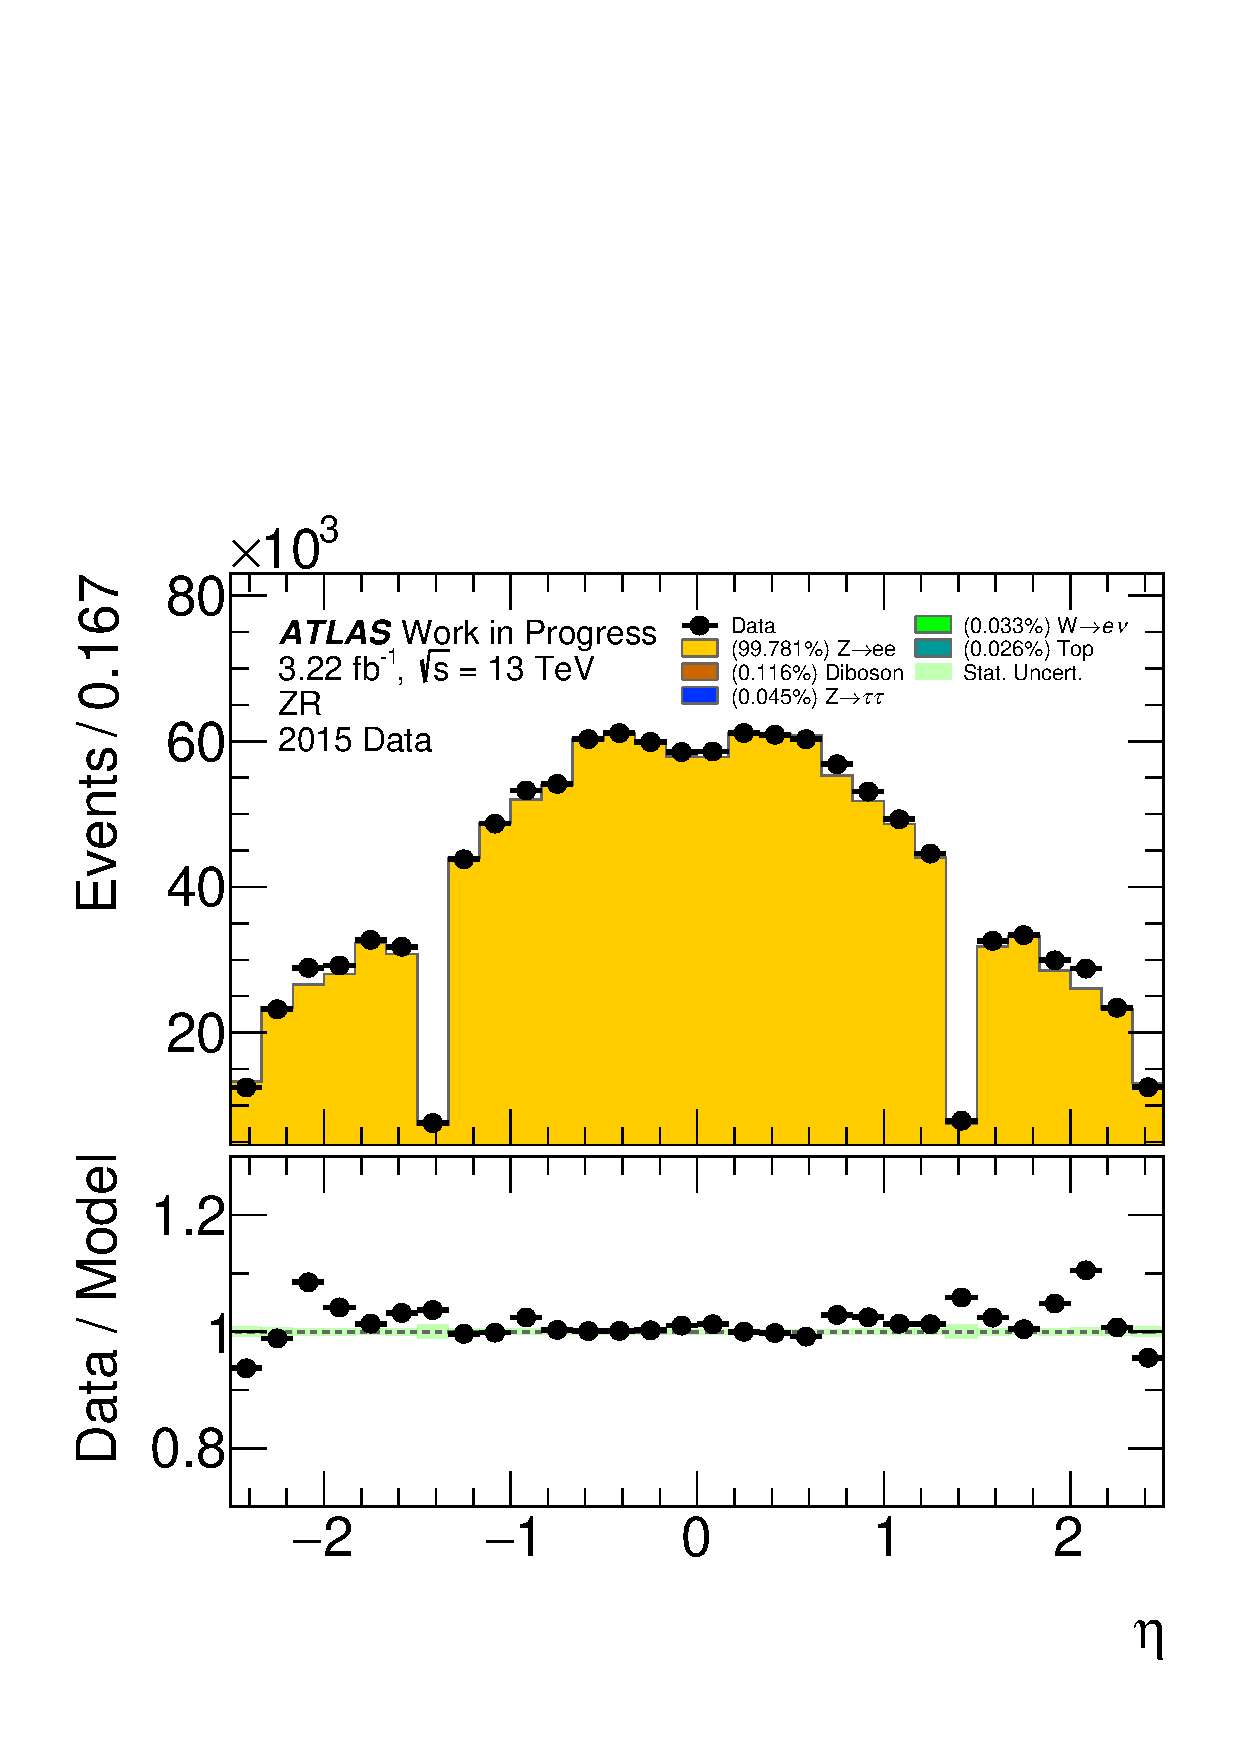
\includegraphics[width=0.45\textwidth]{figures/ZR/dataMc-lep_0_eta-ZR-el.pdf}
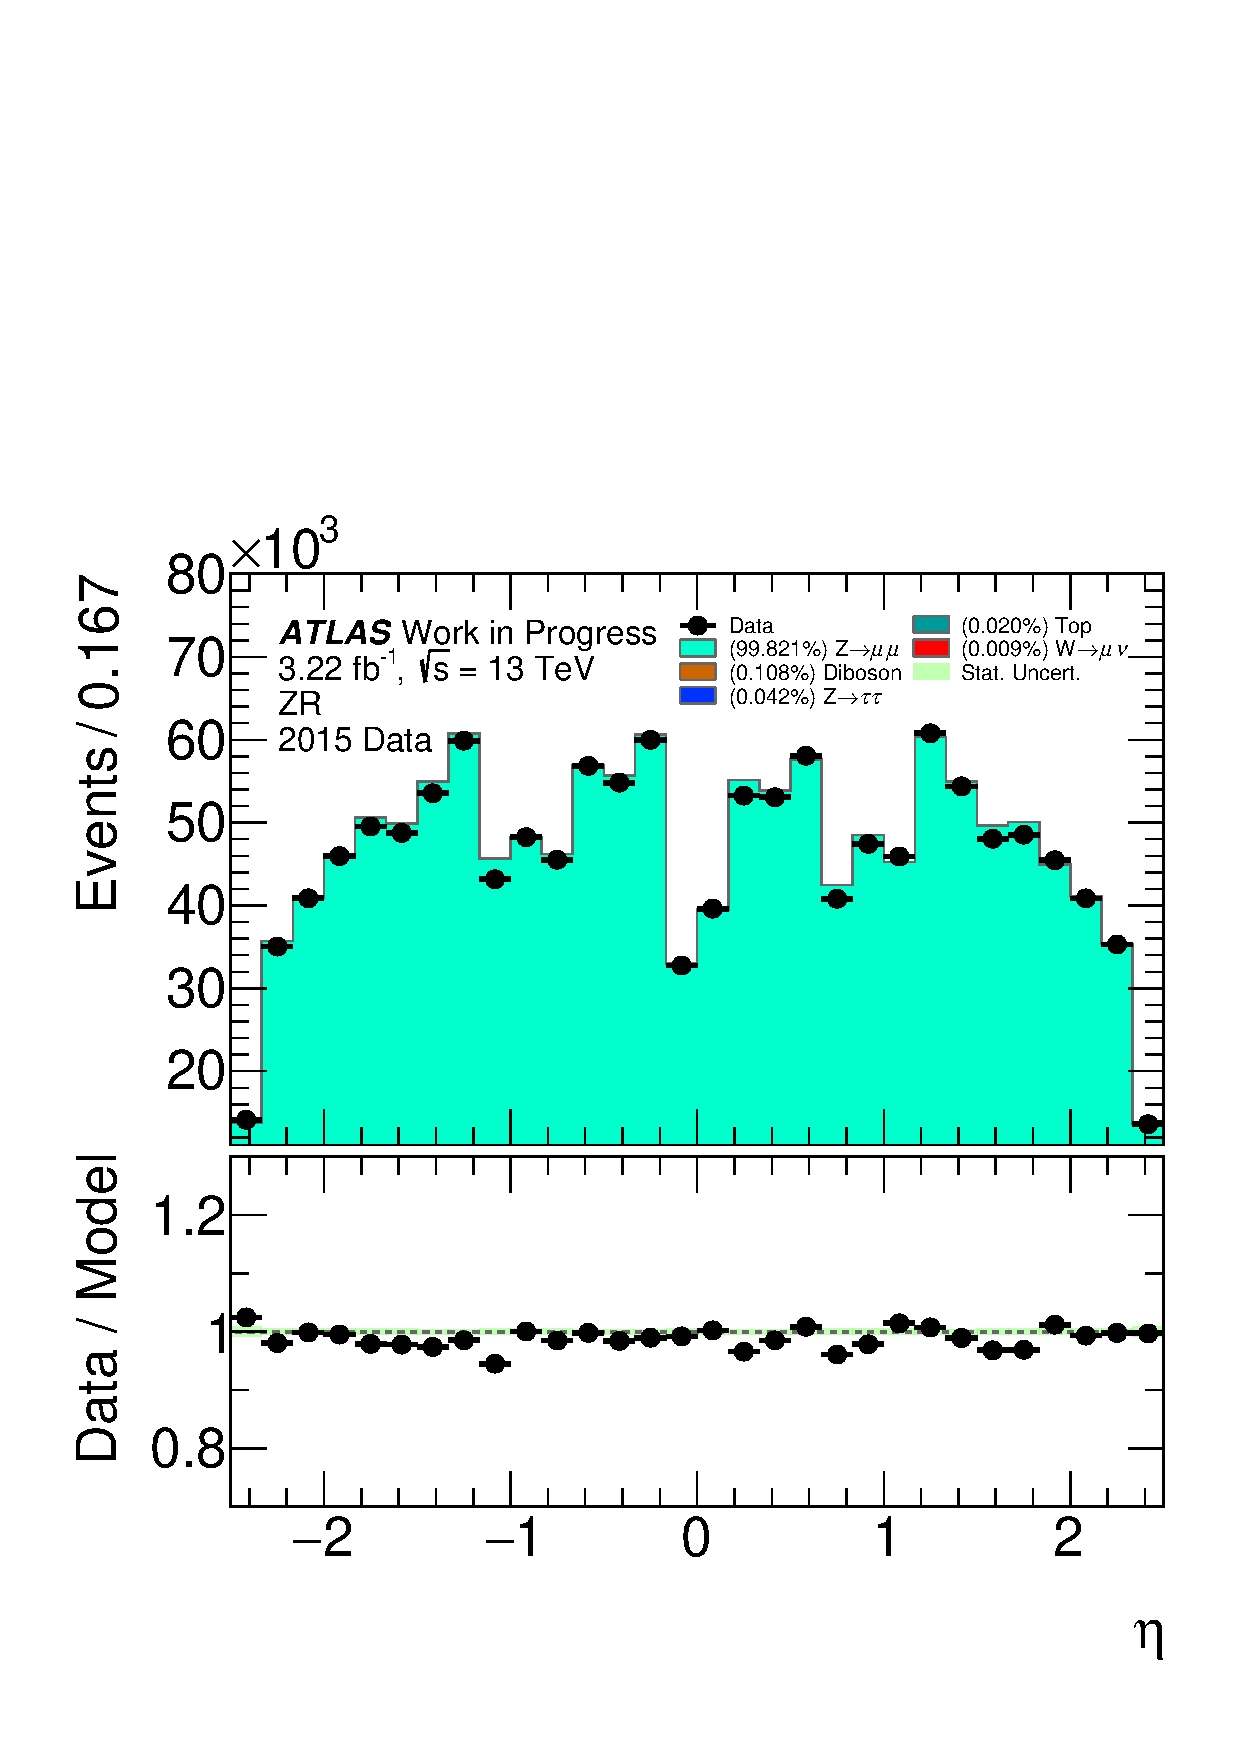
\includegraphics[width=0.45\textwidth]{figures/ZR/dataMc-lep_0_eta-ZR-mu.pdf}
\caption{
Leading lepton pseudorapidity distribution from the $Z \rightarrow e^+e^-$ selection (left) and the $Z \rightarrow \mu^+\mu^-$  selection (right).
The expected contributions from all backgrounds are estimated with Monte Carlo simulations.
The background processes are heavily suppressed and not visible on the linear scale. 
% Systematic uncertainties for the signal and background distributions are combined in the shaded band, and 
Statistical uncertainties are shown on the data points.
Luminosity uncertainties are not included.
}
\label{fig:ZR_lep_0_eta}
\end{figure}

\begin{figure}[htbp]
\centering
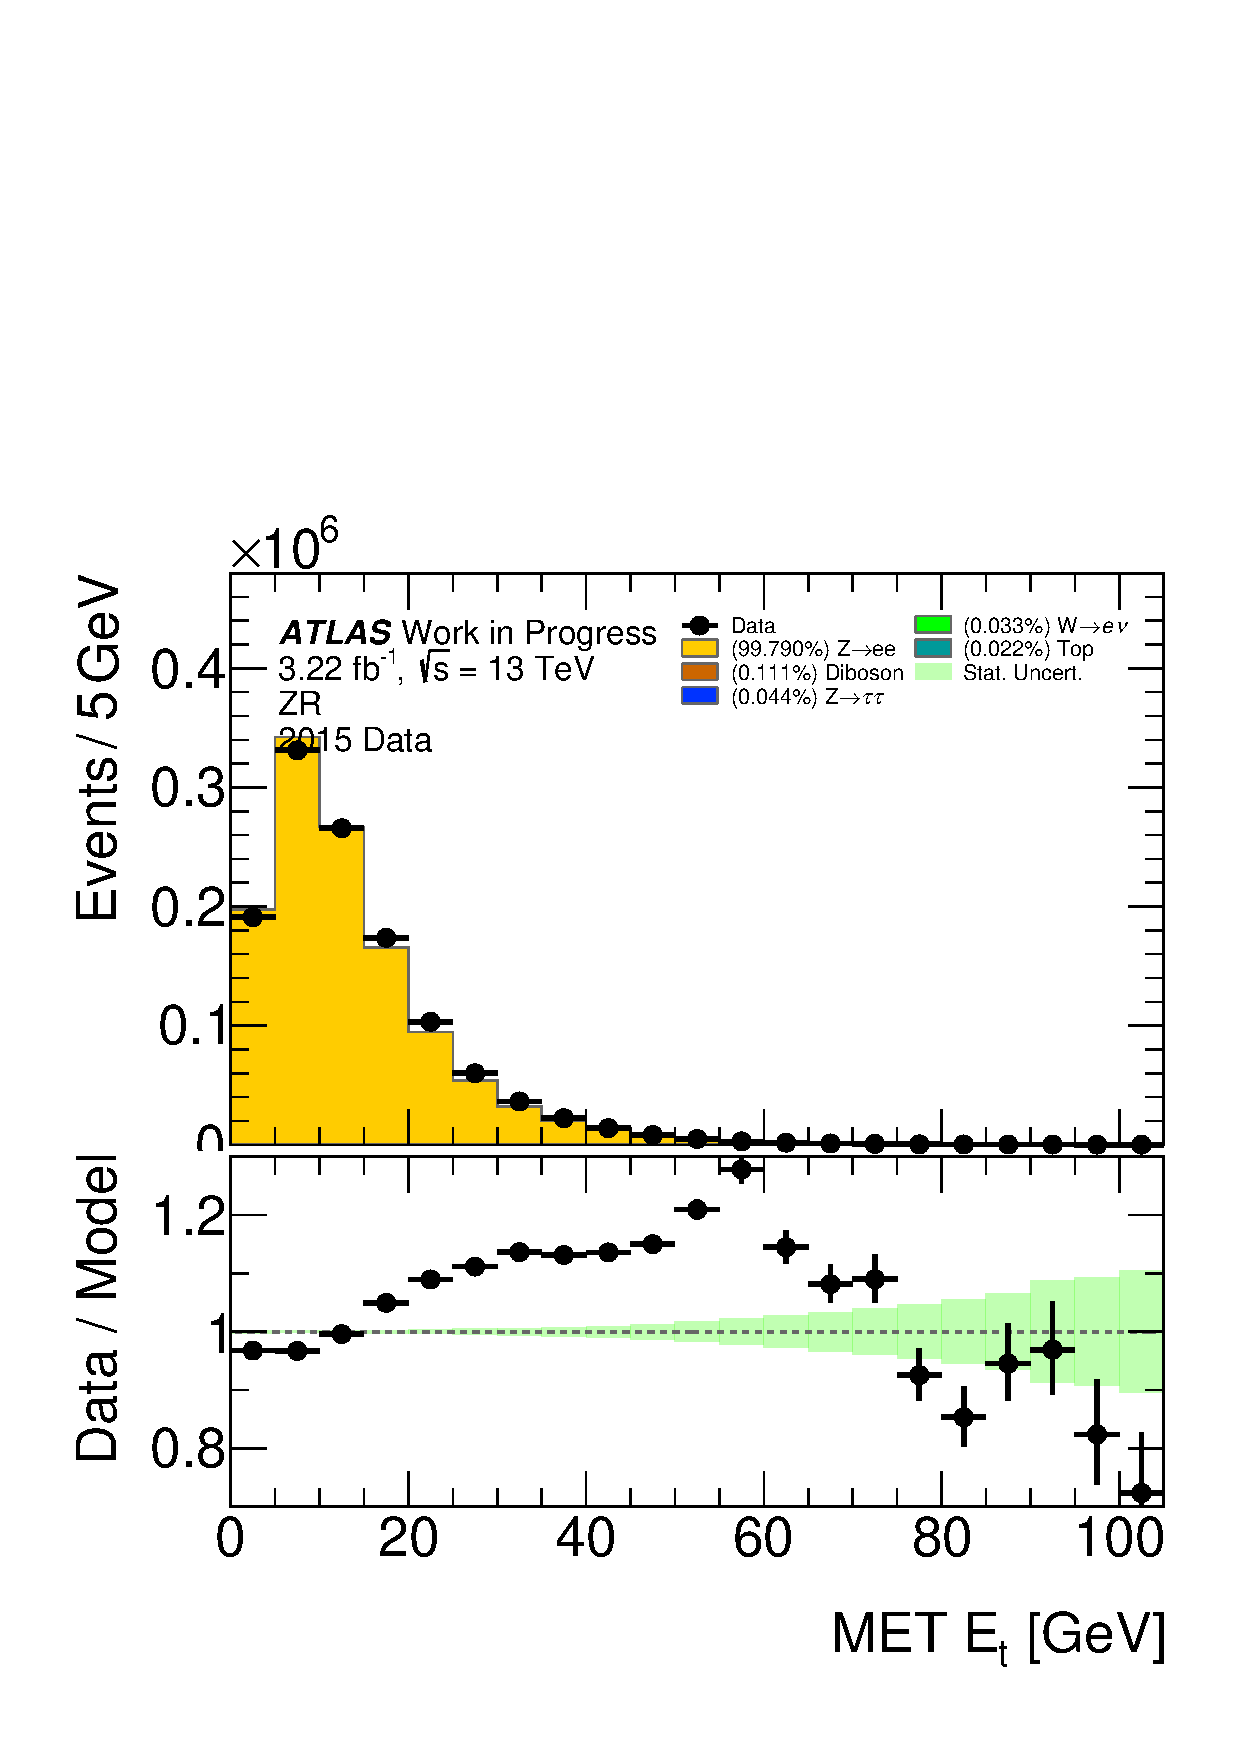
\includegraphics[width=0.45\textwidth]{figures/ZR/dataMc-met_reco_et-ZR-el.pdf}
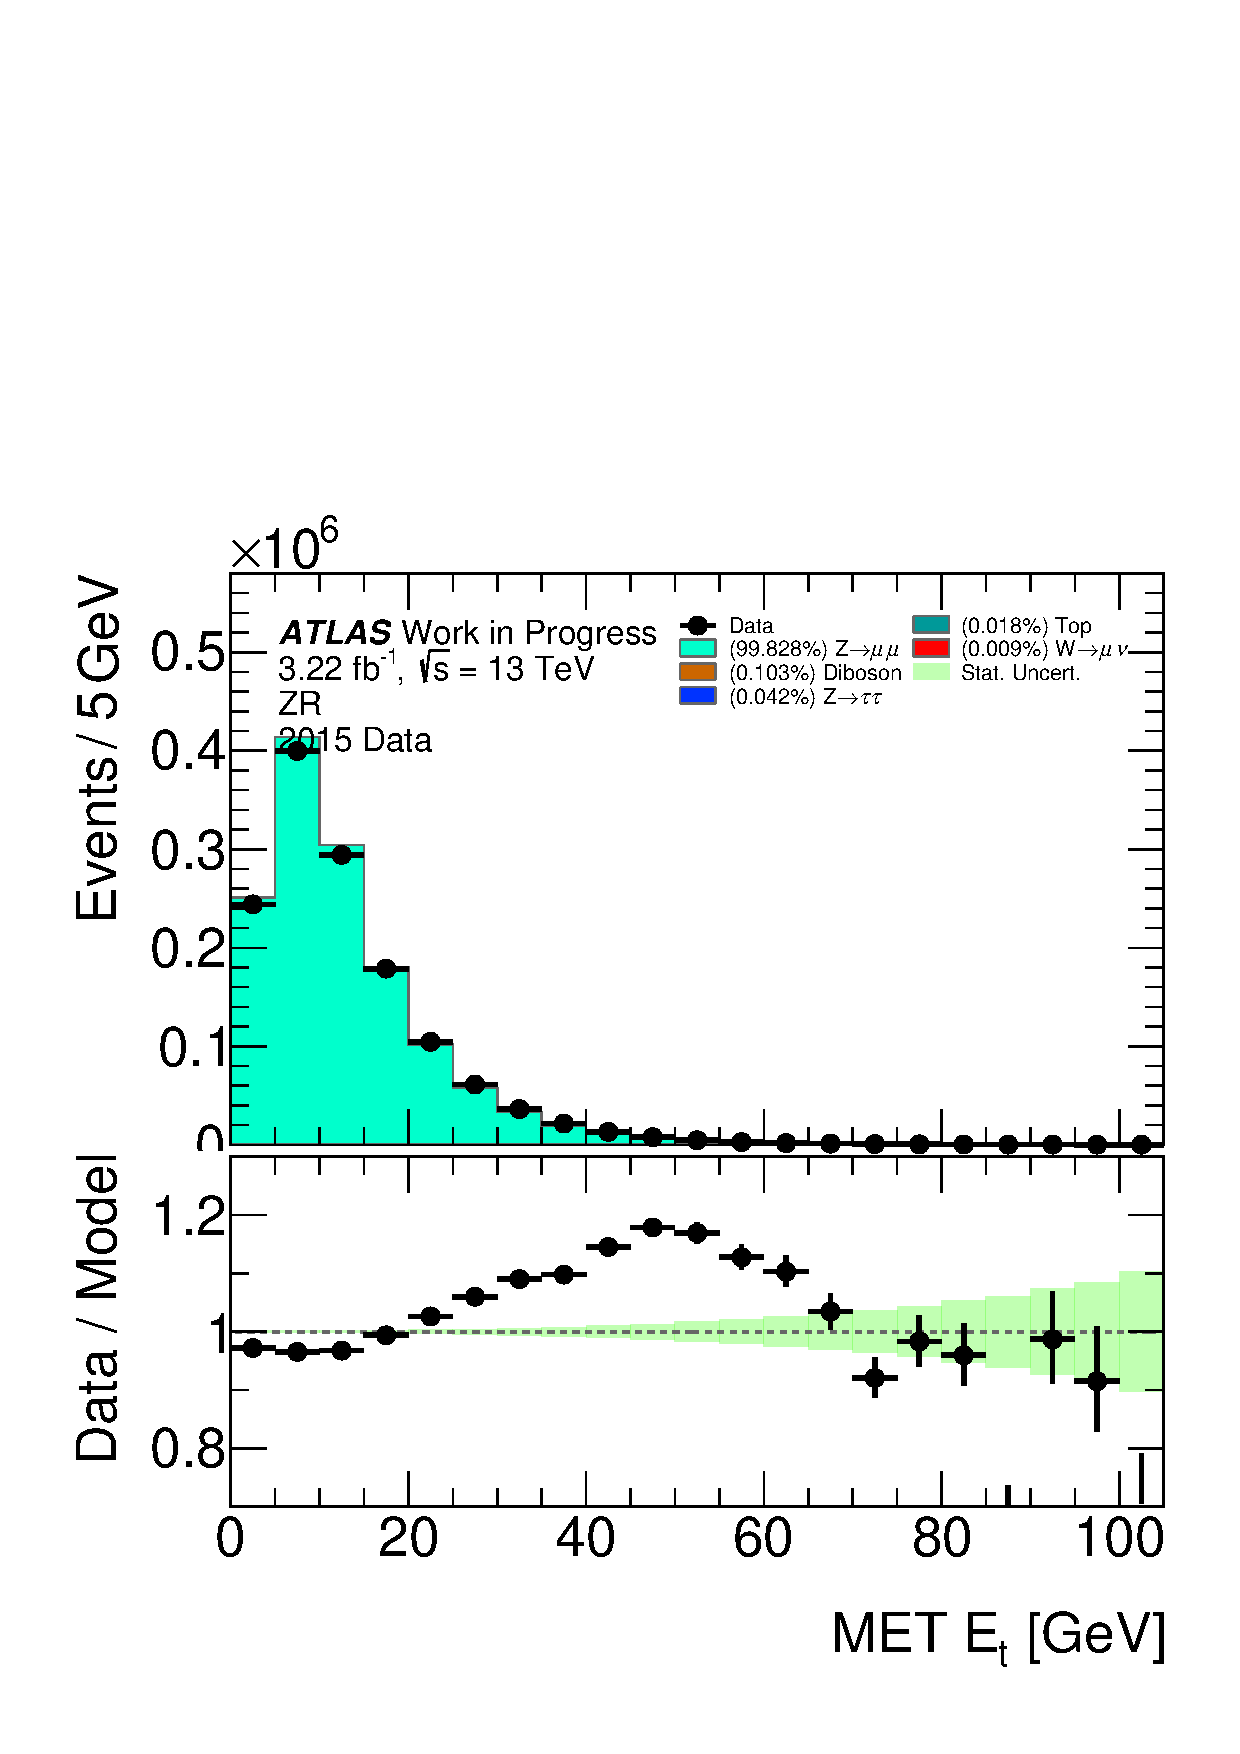
\includegraphics[width=0.45\textwidth]{figures/ZR/dataMc-met_reco_et-ZR-mu.pdf}
\caption{
 Missing transverse energy distribution from the $Z \rightarrow e^+e^-$ selection (left) and the $Z \rightarrow \mu^+\mu^-$  selection (right).
The expected contributions from all backgrounds are estimated with Monte Carlo simulations.
The background processes are heavily suppressed and not visible on the linear scale. 
% Systematic uncertainties for the signal and background distributions are combined in the shaded band, and 
Statistical uncertainties are shown on the data points.
Luminosity uncertainties are not included.
}
\label{fig:ZR_met_reco_et}
\end{figure}

\begin{figure}[htbp]
\centering
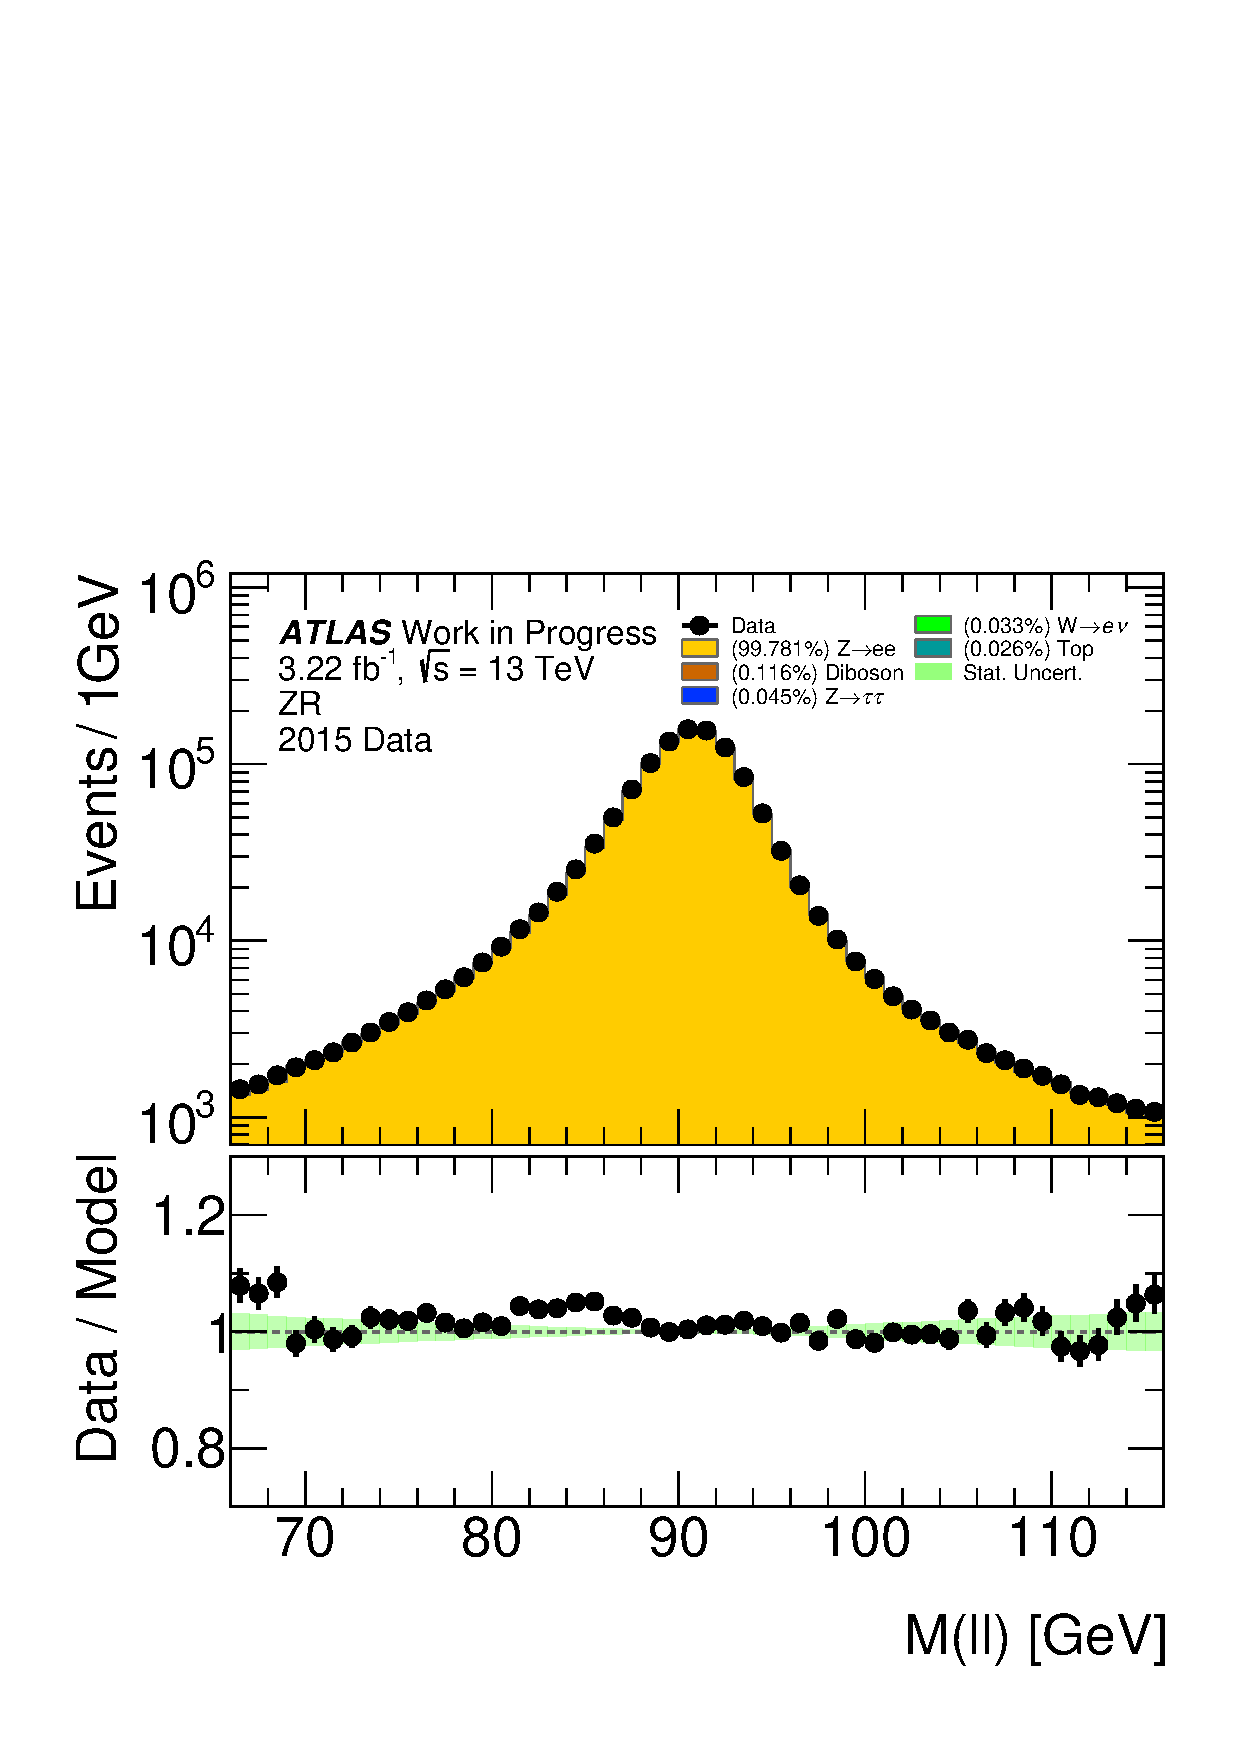
\includegraphics[width=0.45\textwidth]{figures/ZR/dataMc-dilep_m-ZR-el-log.pdf}
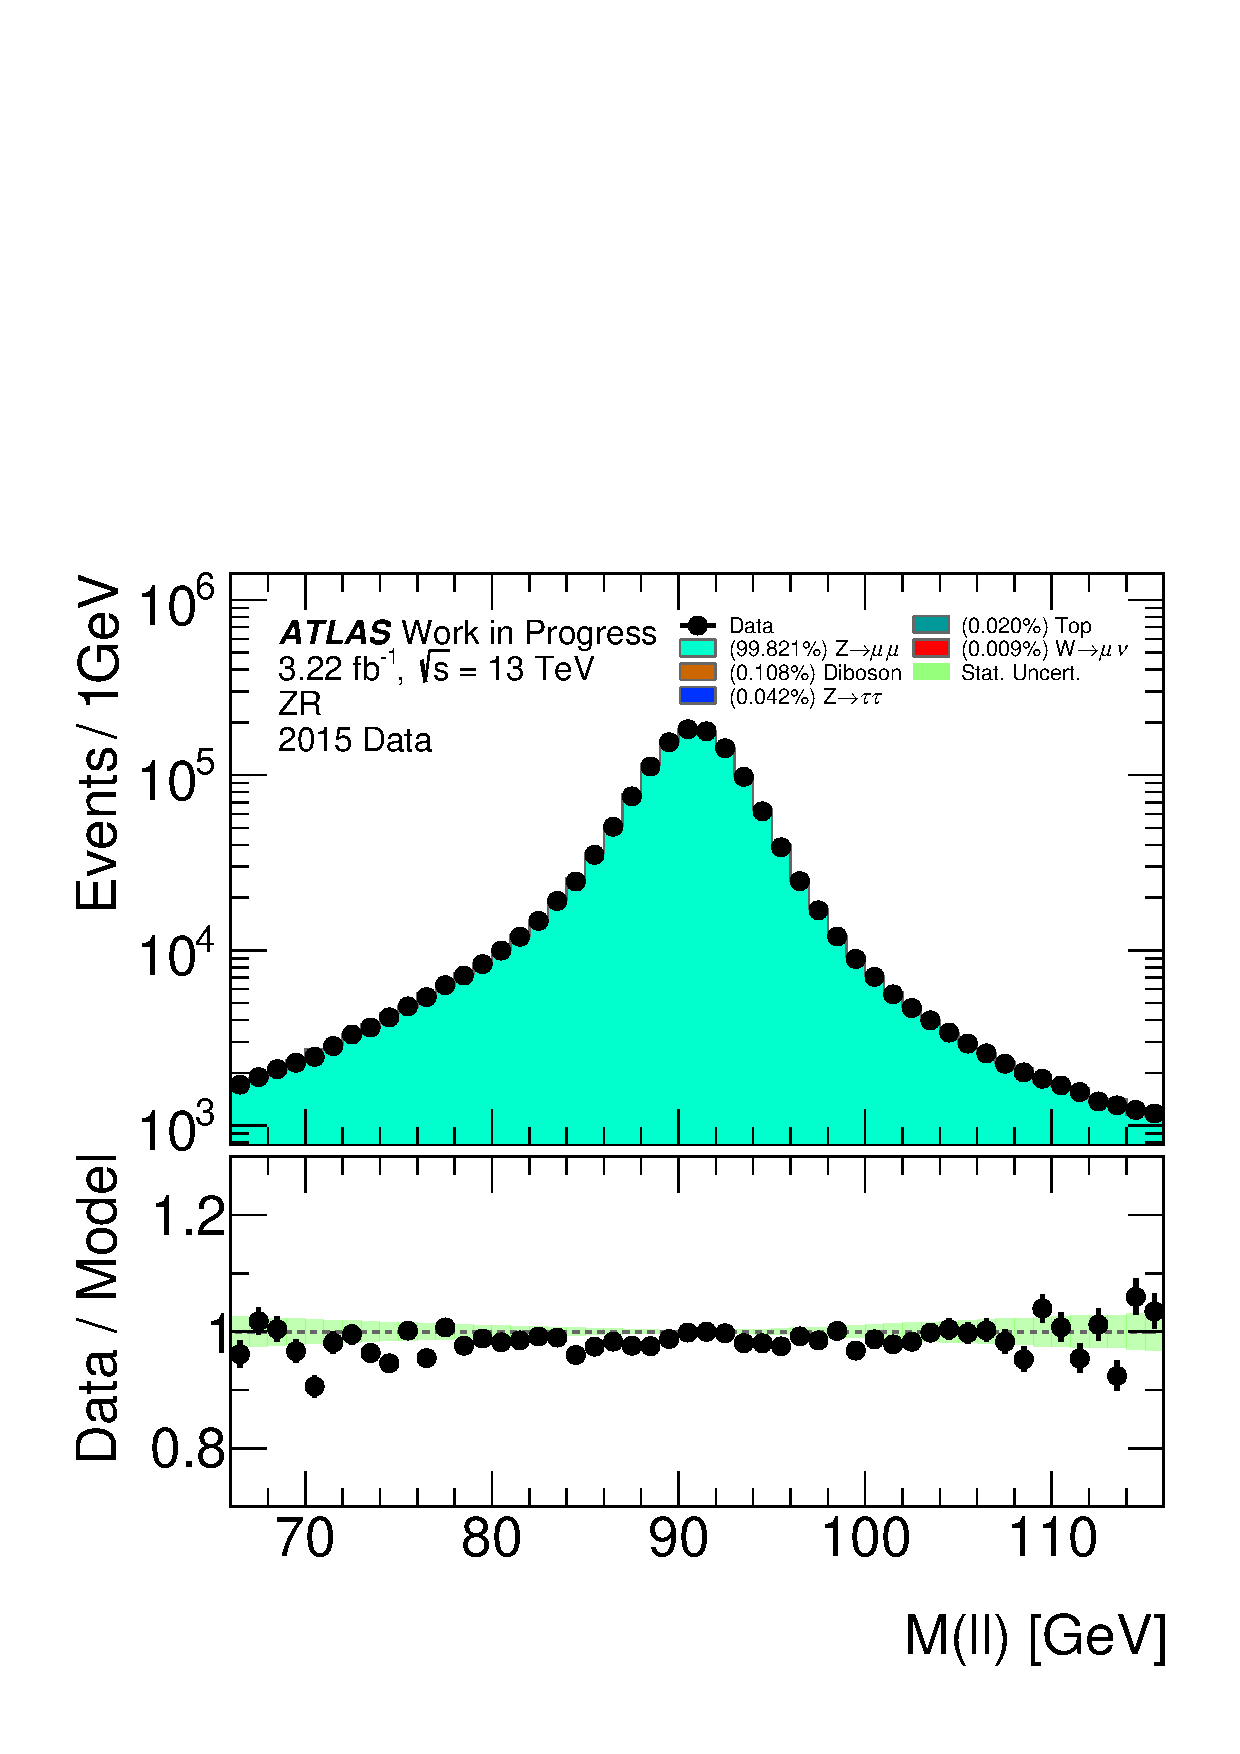
\includegraphics[width=0.45\textwidth]{figures/ZR/dataMc-dilep_m-ZR-mu-log.pdf}
\caption{
Dilepton mass distribution after the $Z \rightarrow e^+e^-$ selection (left) and the $Z \rightarrow \mu^+\mu^-$  selection (right).
Both leptons is required to satisfy $p_T > 27$ GeV.
The expected contributions from all backgrounds are estimated with Monte Carlo simulations.
% The background processes are heavily suppressed and not visible on the linear scale. 
% Systematic uncertainties for the signal and background distributions are combined in the shaded band, and 
Statistical uncertainties are shown on the data points.
Luminosity uncertainties are not included.
}
\label{fig:ZR_dilep_m_log}
\end{figure}

\begin{figure}[htbp]
\centering
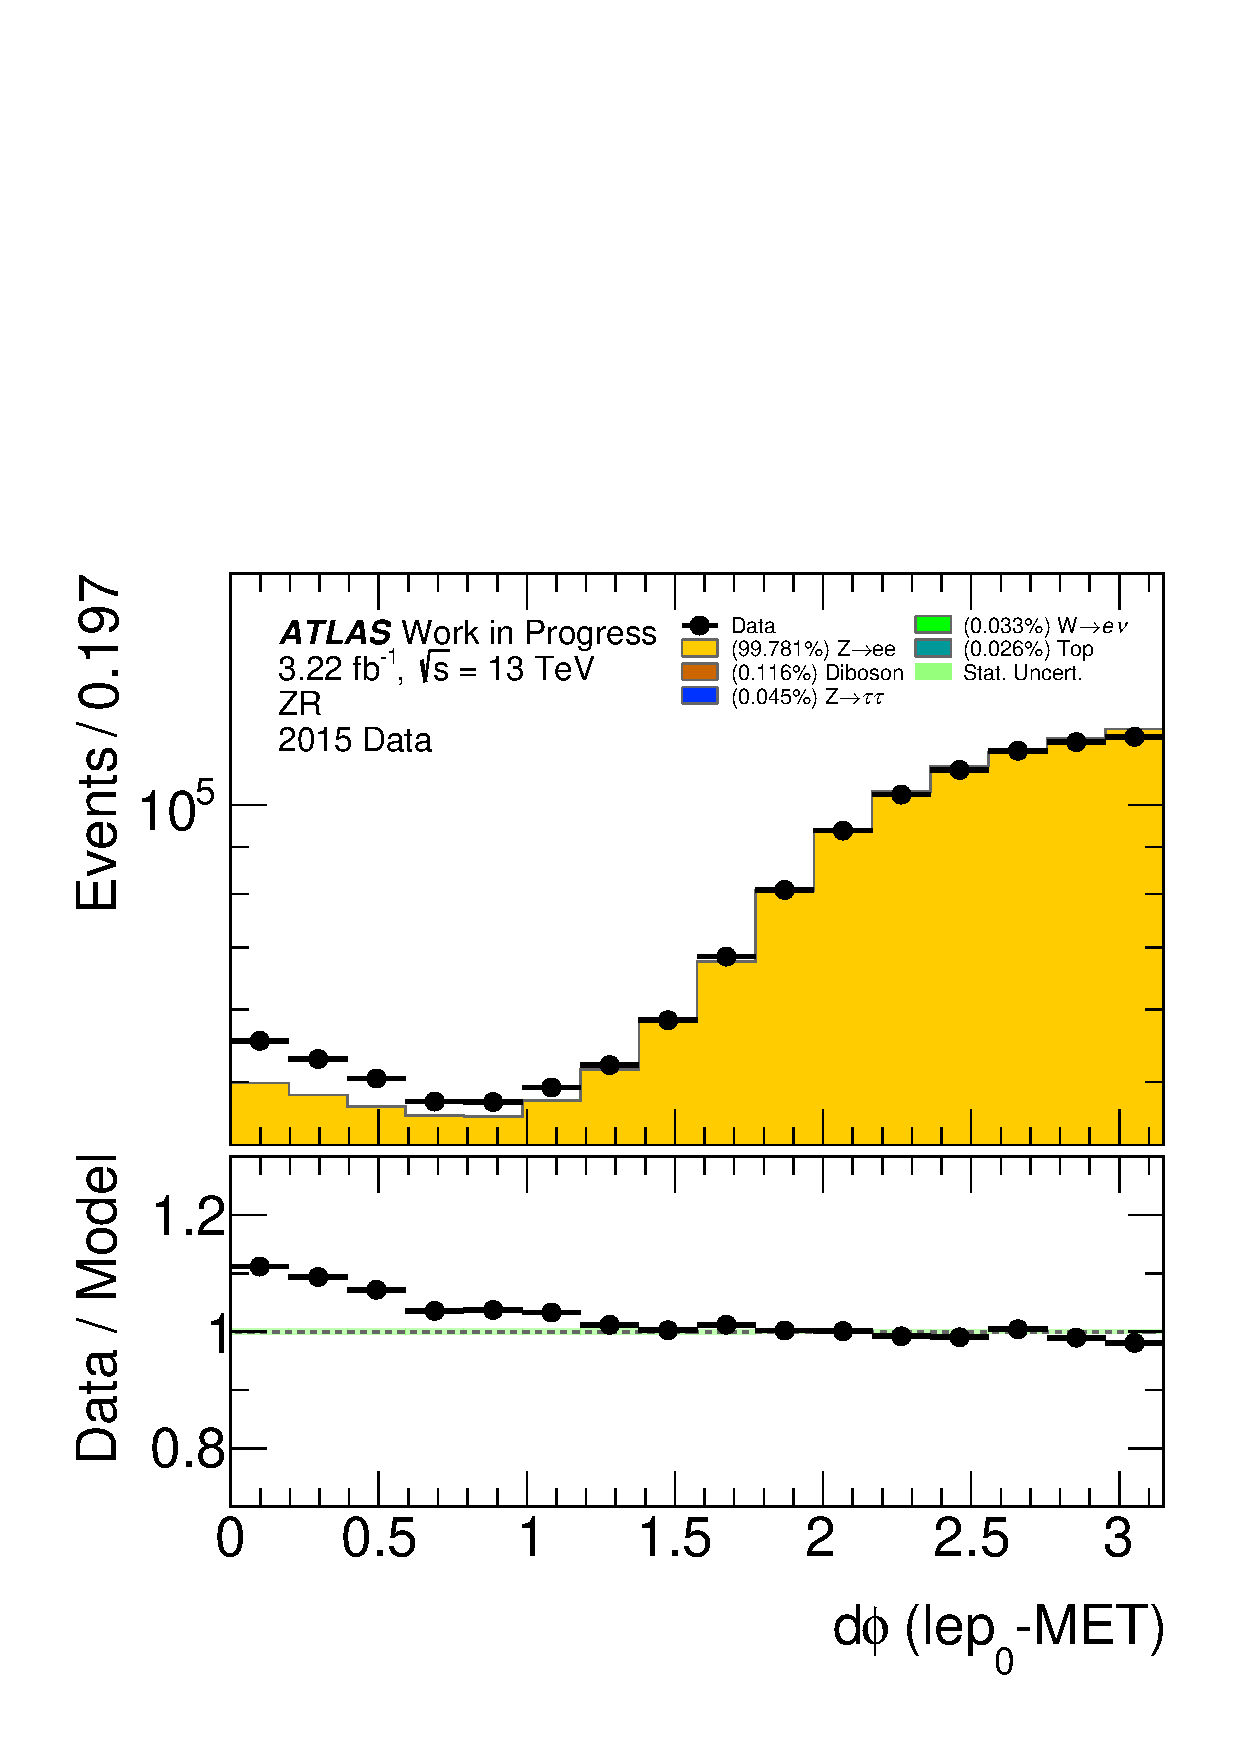
\includegraphics[width=0.45\textwidth]{figures/ZR/dataMc-lepmet_dphi-ZR-el-log.pdf}
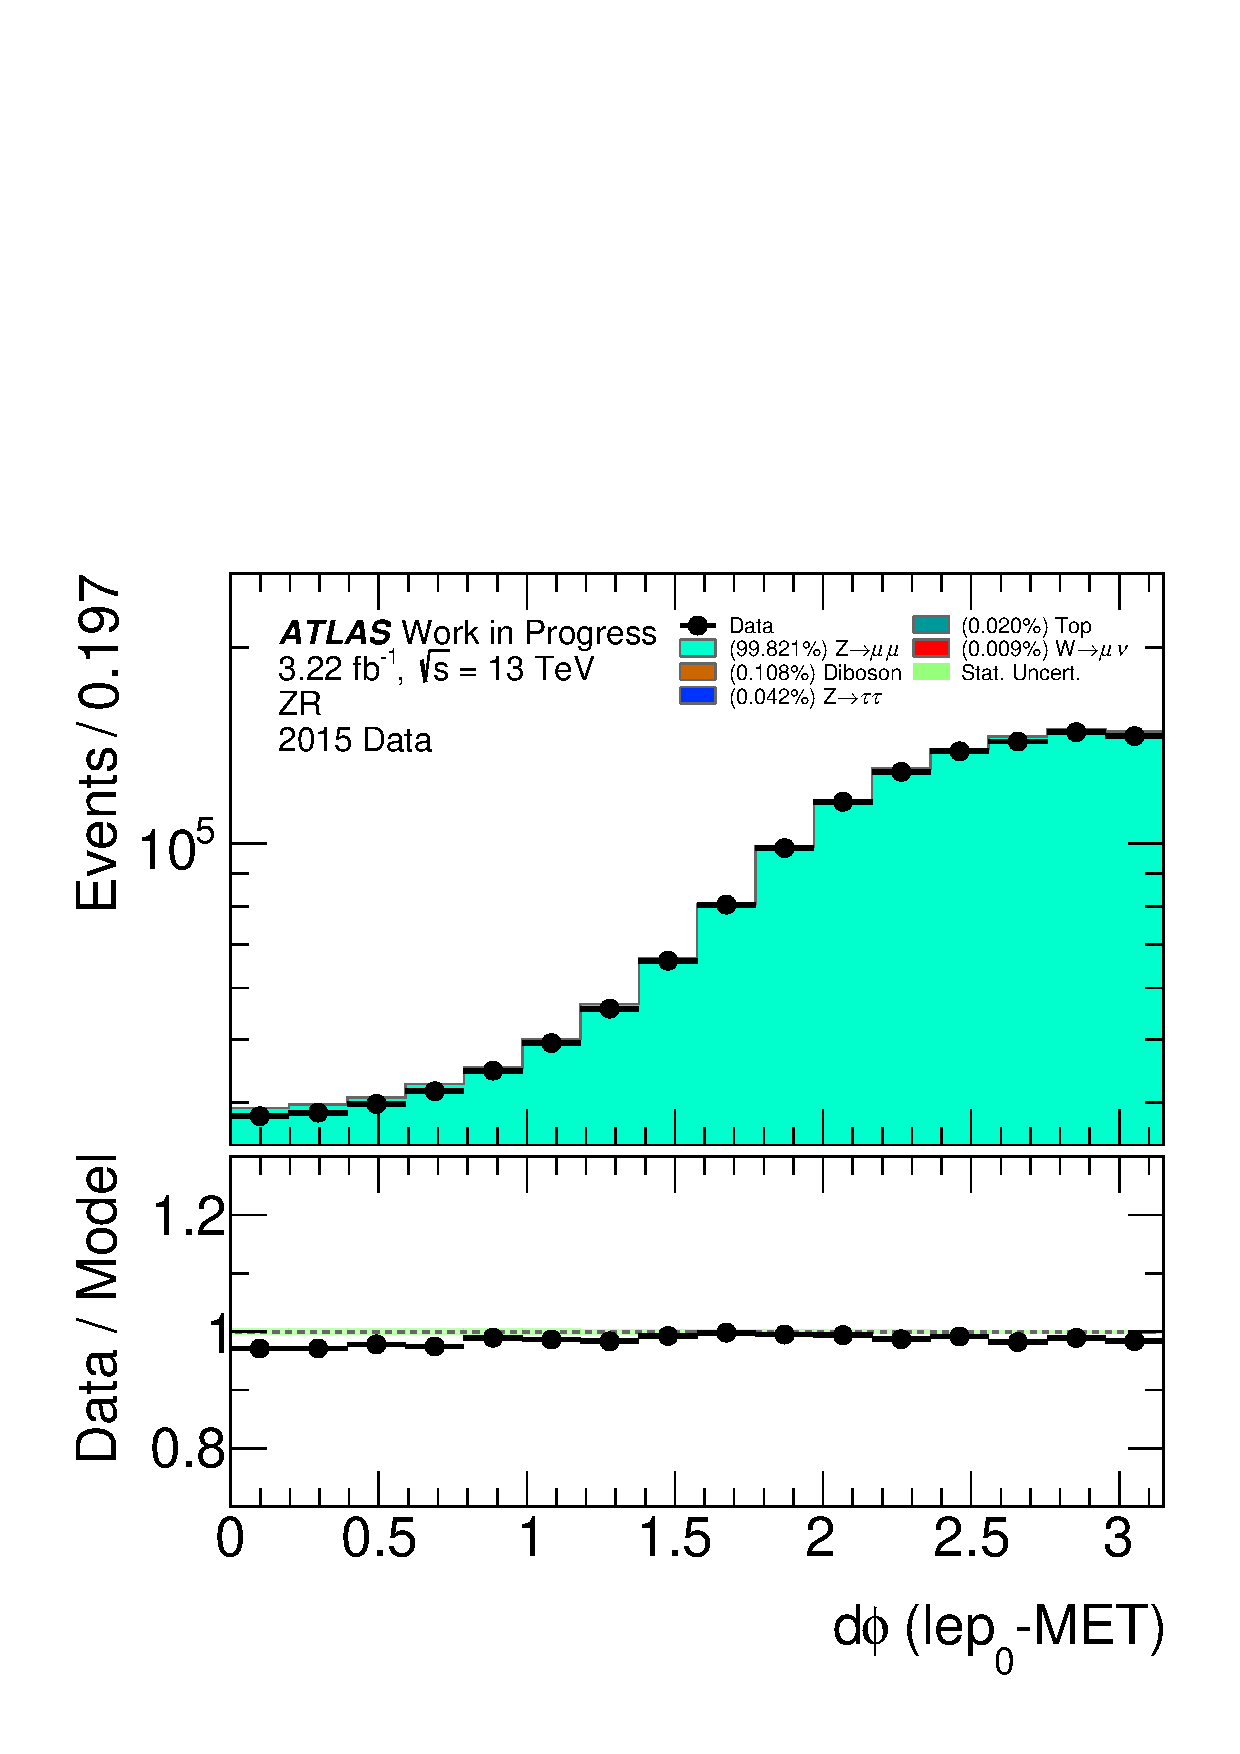
\includegraphics[width=0.45\textwidth]{figures/ZR/dataMc-lepmet_dphi-ZR-mu-log.pdf}
\caption{
Azimuthal angle distribution, calculated as azimuthal angle difference of the leading lepton and the $E_{T}^{miss}$ from the $Z \rightarrow e^+e^-$ selection (left) and the $Z \rightarrow \mu^+\mu^-$  selection (right).
The $E_{T}^{miss}$ has been recalibrated using the best energy calibration for each of the identified physics objects.
The expected contributions from all backgrounds are estimated with Monte Carlo simulations. 
% Systematic uncertainties for the signal and background distributions are combined in the shaded band, and 
Statistical uncertainties are shown on the data points.
Luminosity uncertainties are not included.
}
\label{fig:ZR_lepmet_dphi}
\end{figure}

\begin{figure}[htbp]
\centering
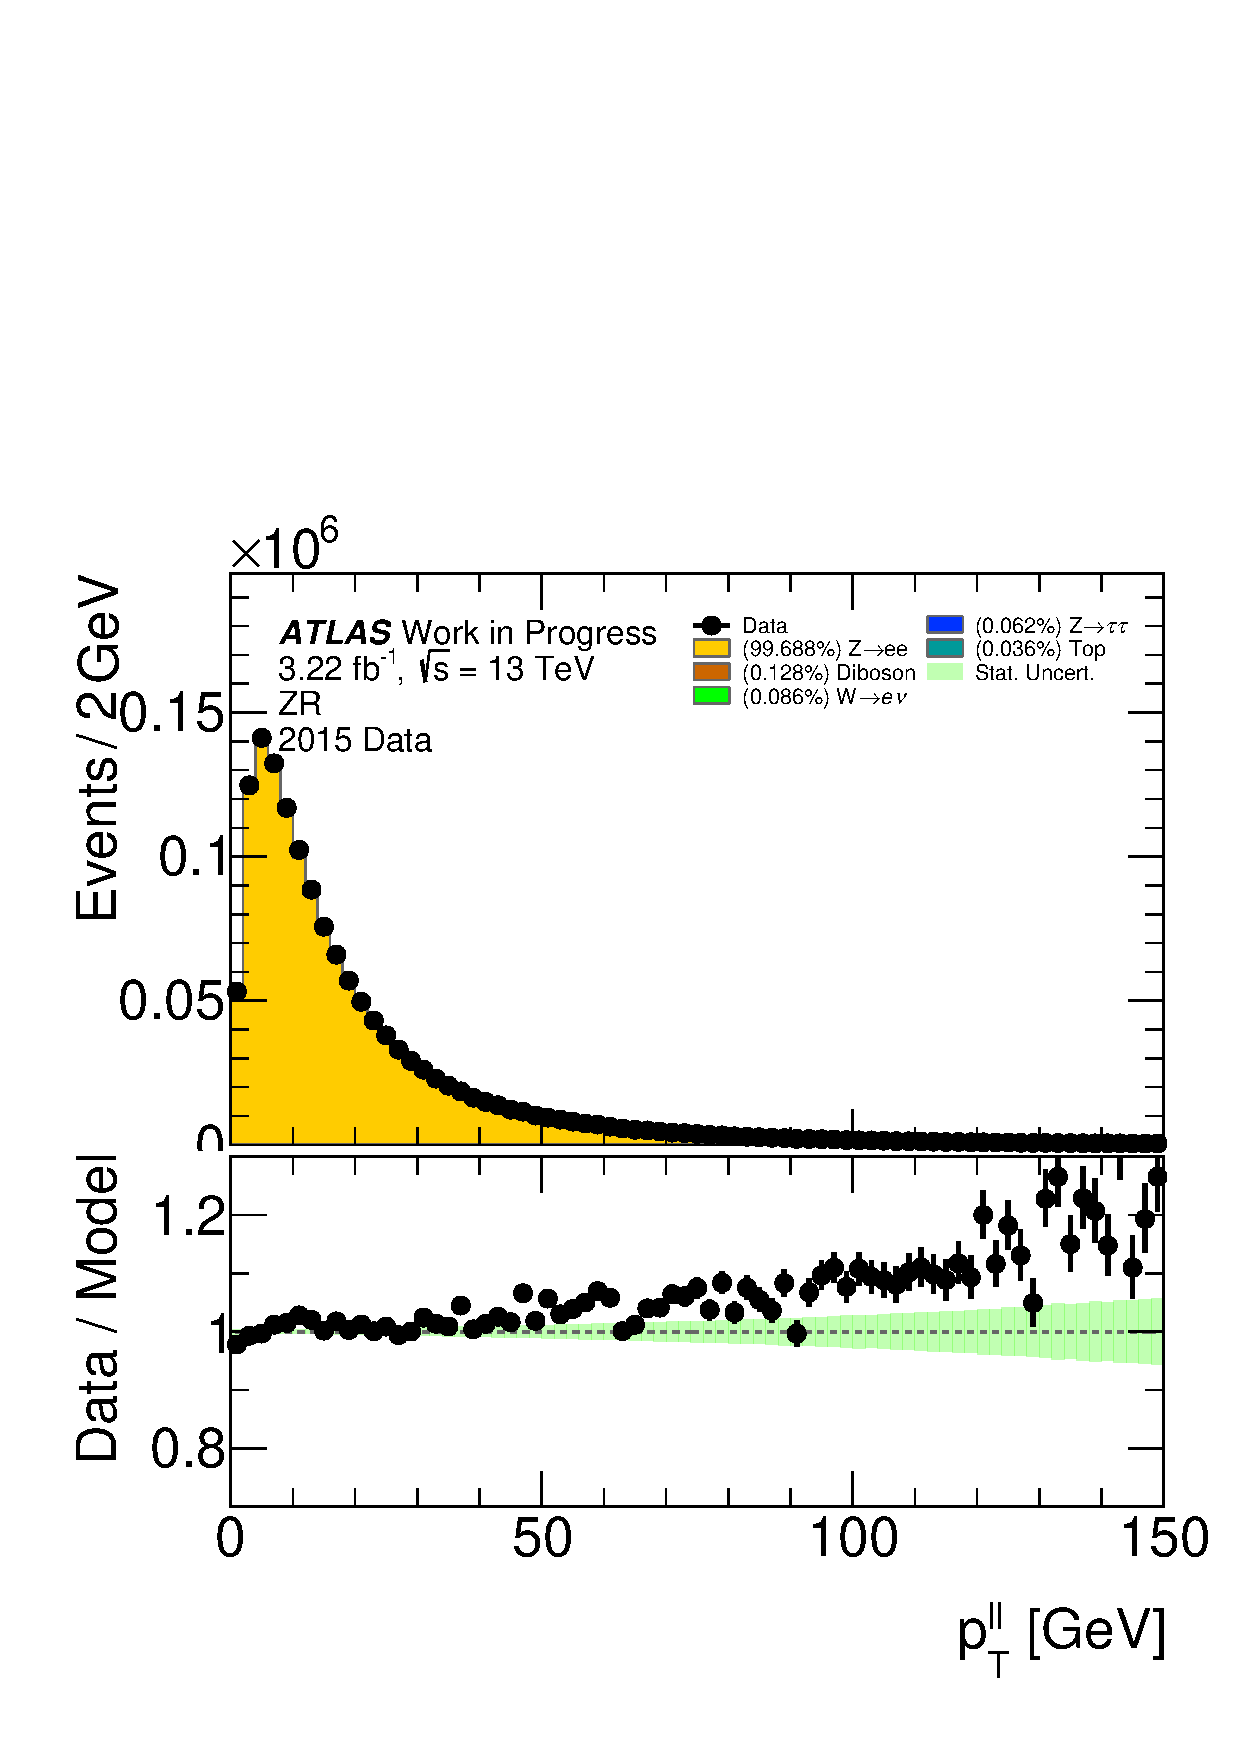
\includegraphics[width=0.45\textwidth]{figures/ZR/dataMc-dilep_pt-ZR-el.pdf}
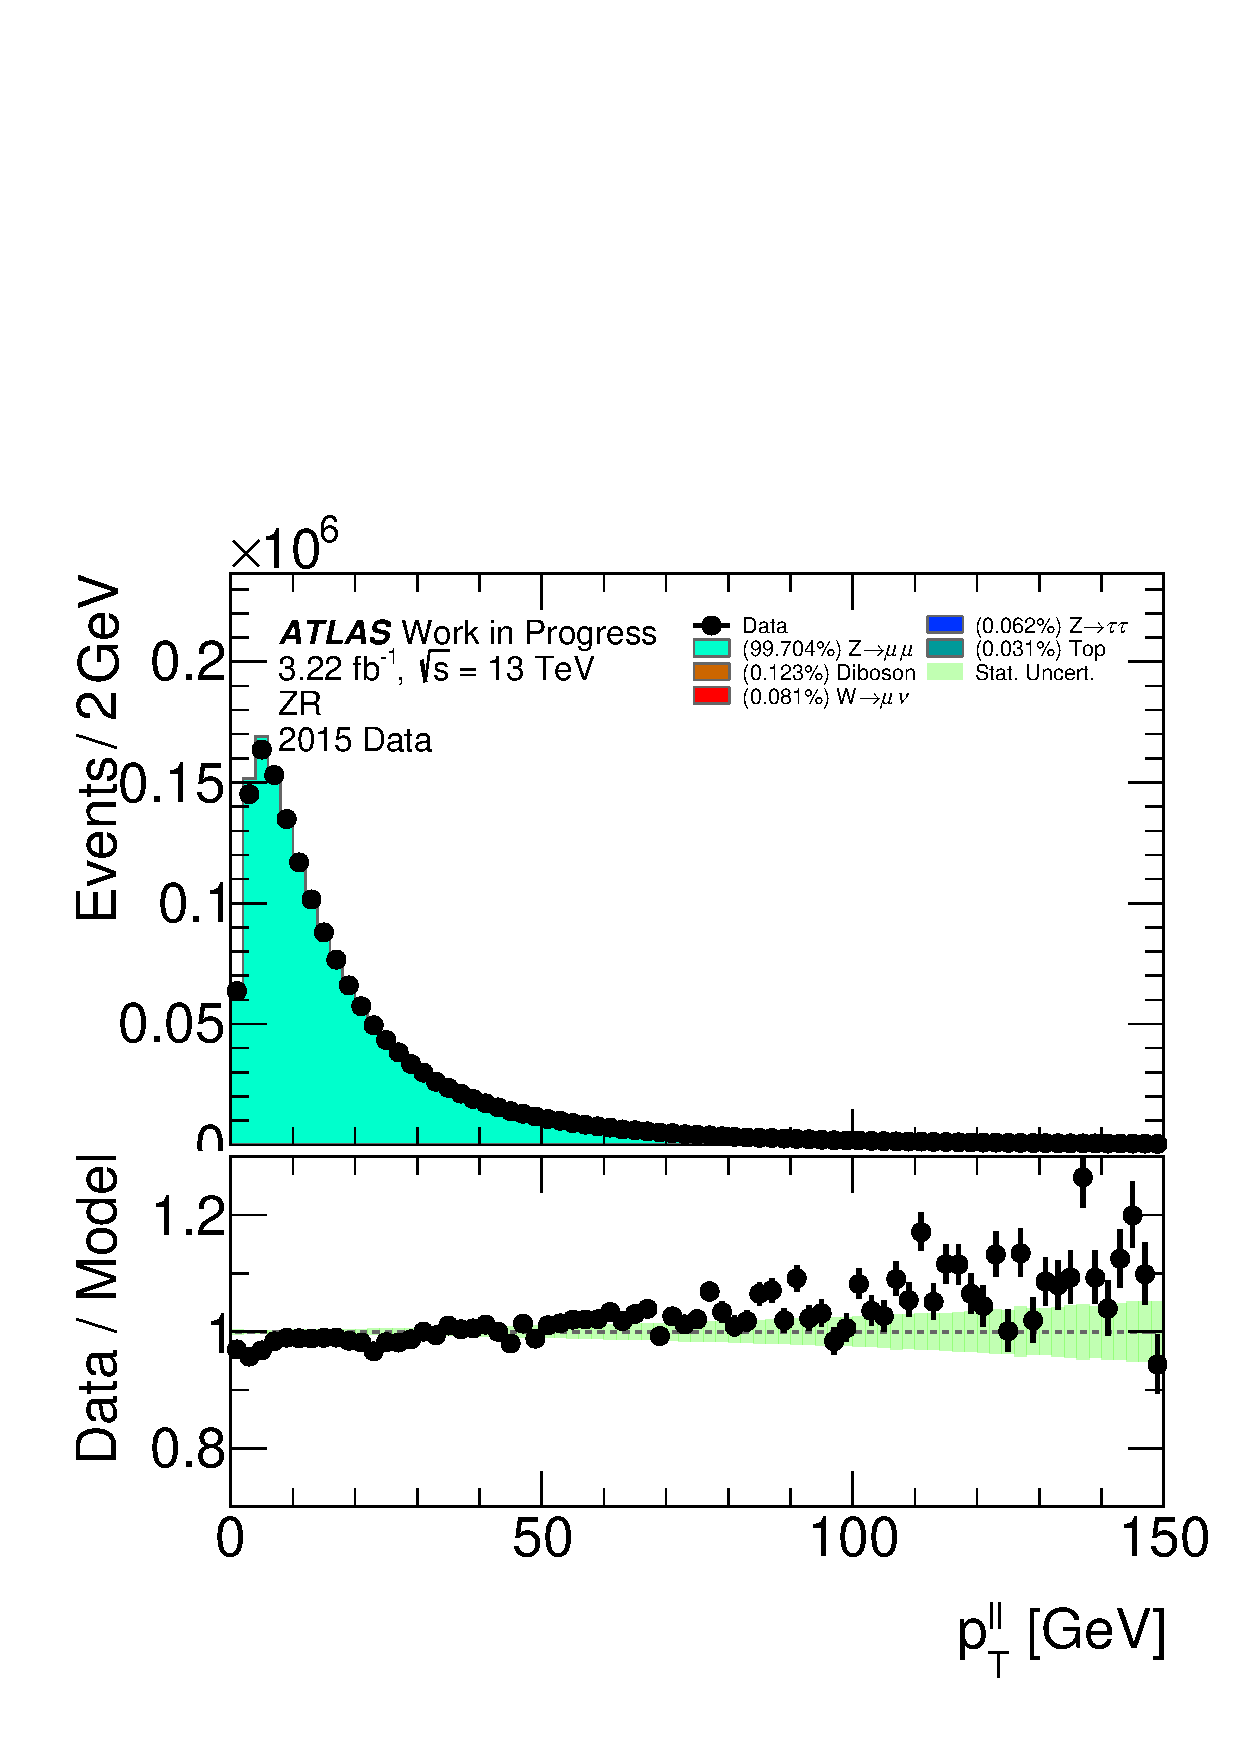
\includegraphics[width=0.45\textwidth]{figures/ZR/dataMc-dilep_pt-ZR-mu.pdf}
\caption{
Z boson transverse momentum distribution after the $Z \rightarrow e^+e^-$ selection (left) and the $Z \rightarrow \mu^+\mu^-$  selection (right).
The expected contributions from all backgrounds are estimated with Monte Carlo simulations.
The background processes are heavily suppressed and not visible on the linear scale. 
% Systematic uncertainties for the signal and background distributions are combined in the shaded band, and 
Statistical uncertainties are shown on the data points.
Luminosity uncertainties are not included.
}
\label{fig:ZR_dilep_pt}
\end{figure}

\begin{figure}[htbp]
\centering
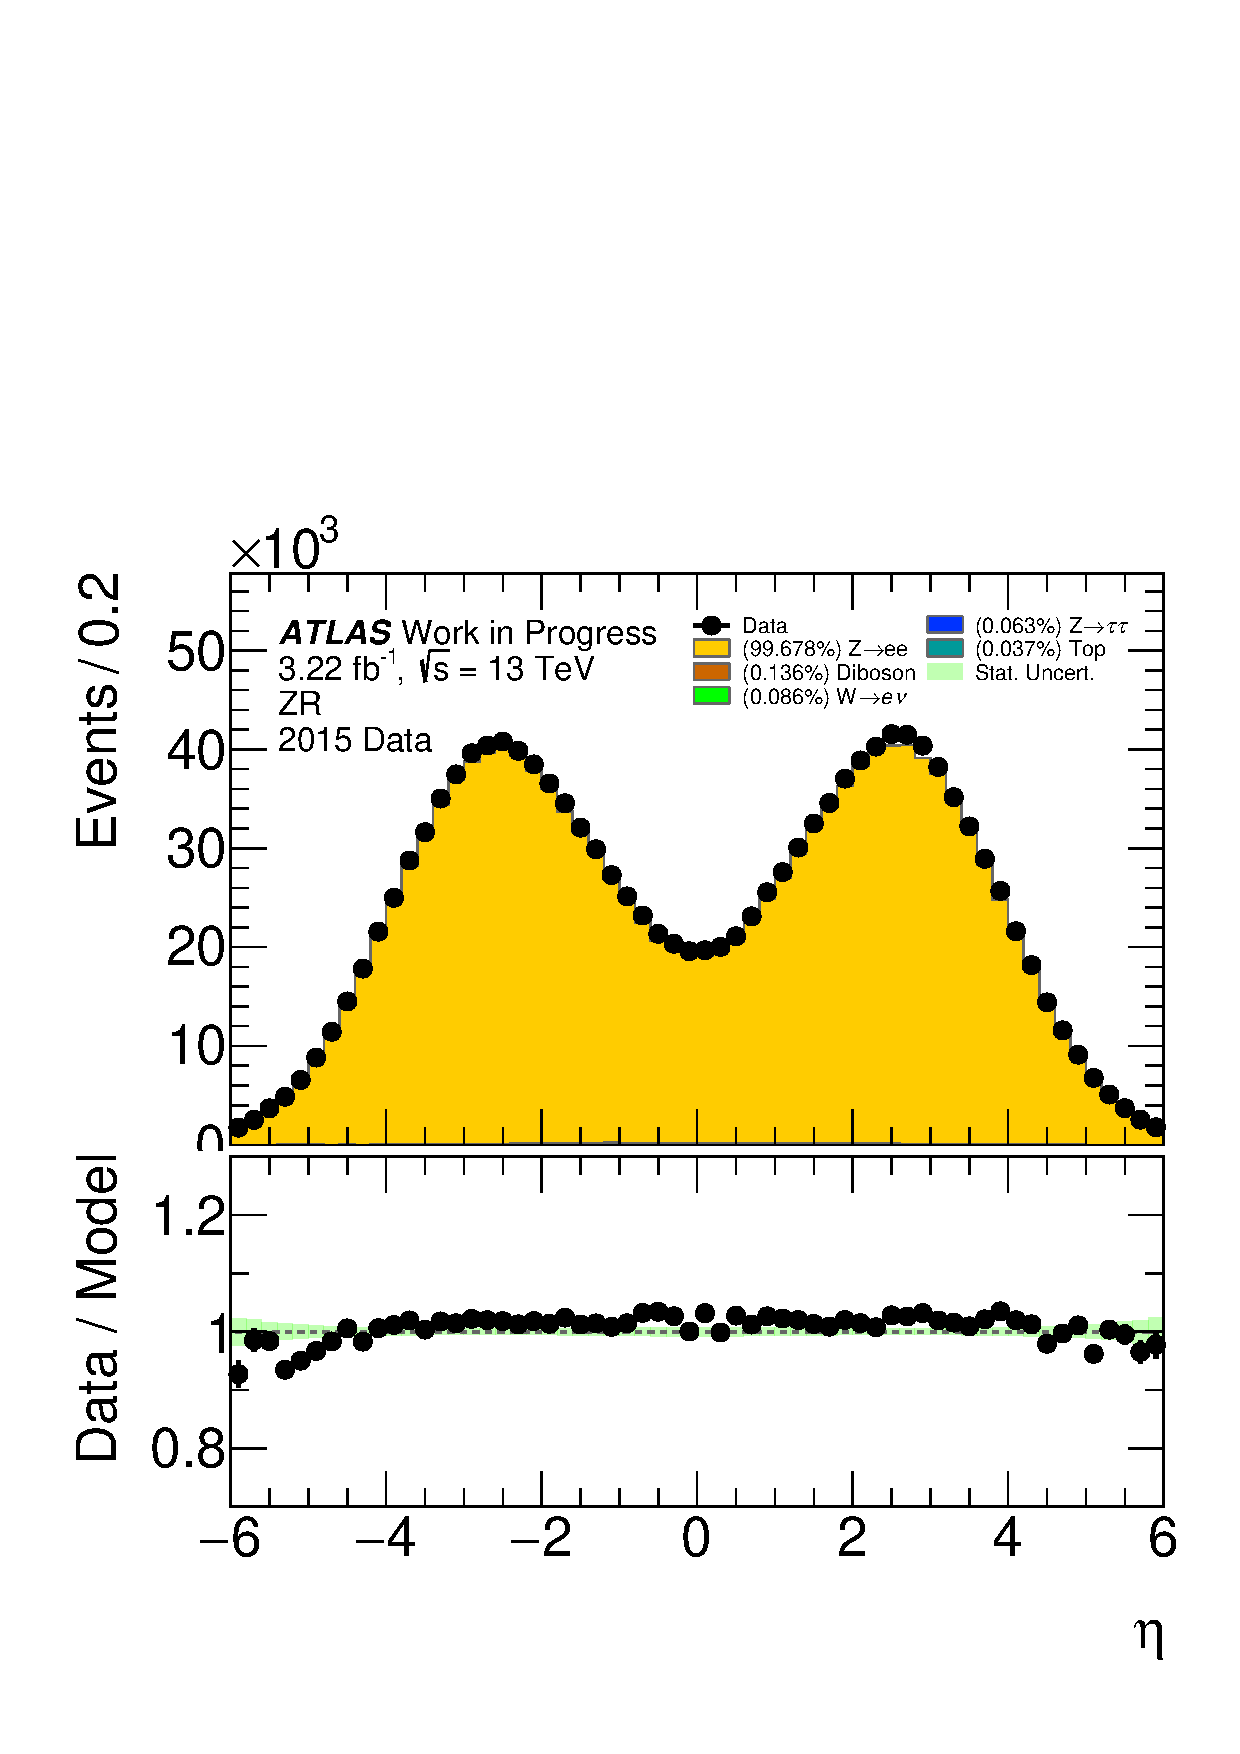
\includegraphics[width=0.45\textwidth]{figures/ZR/dataMc-dilep_eta-ZR-el.pdf}
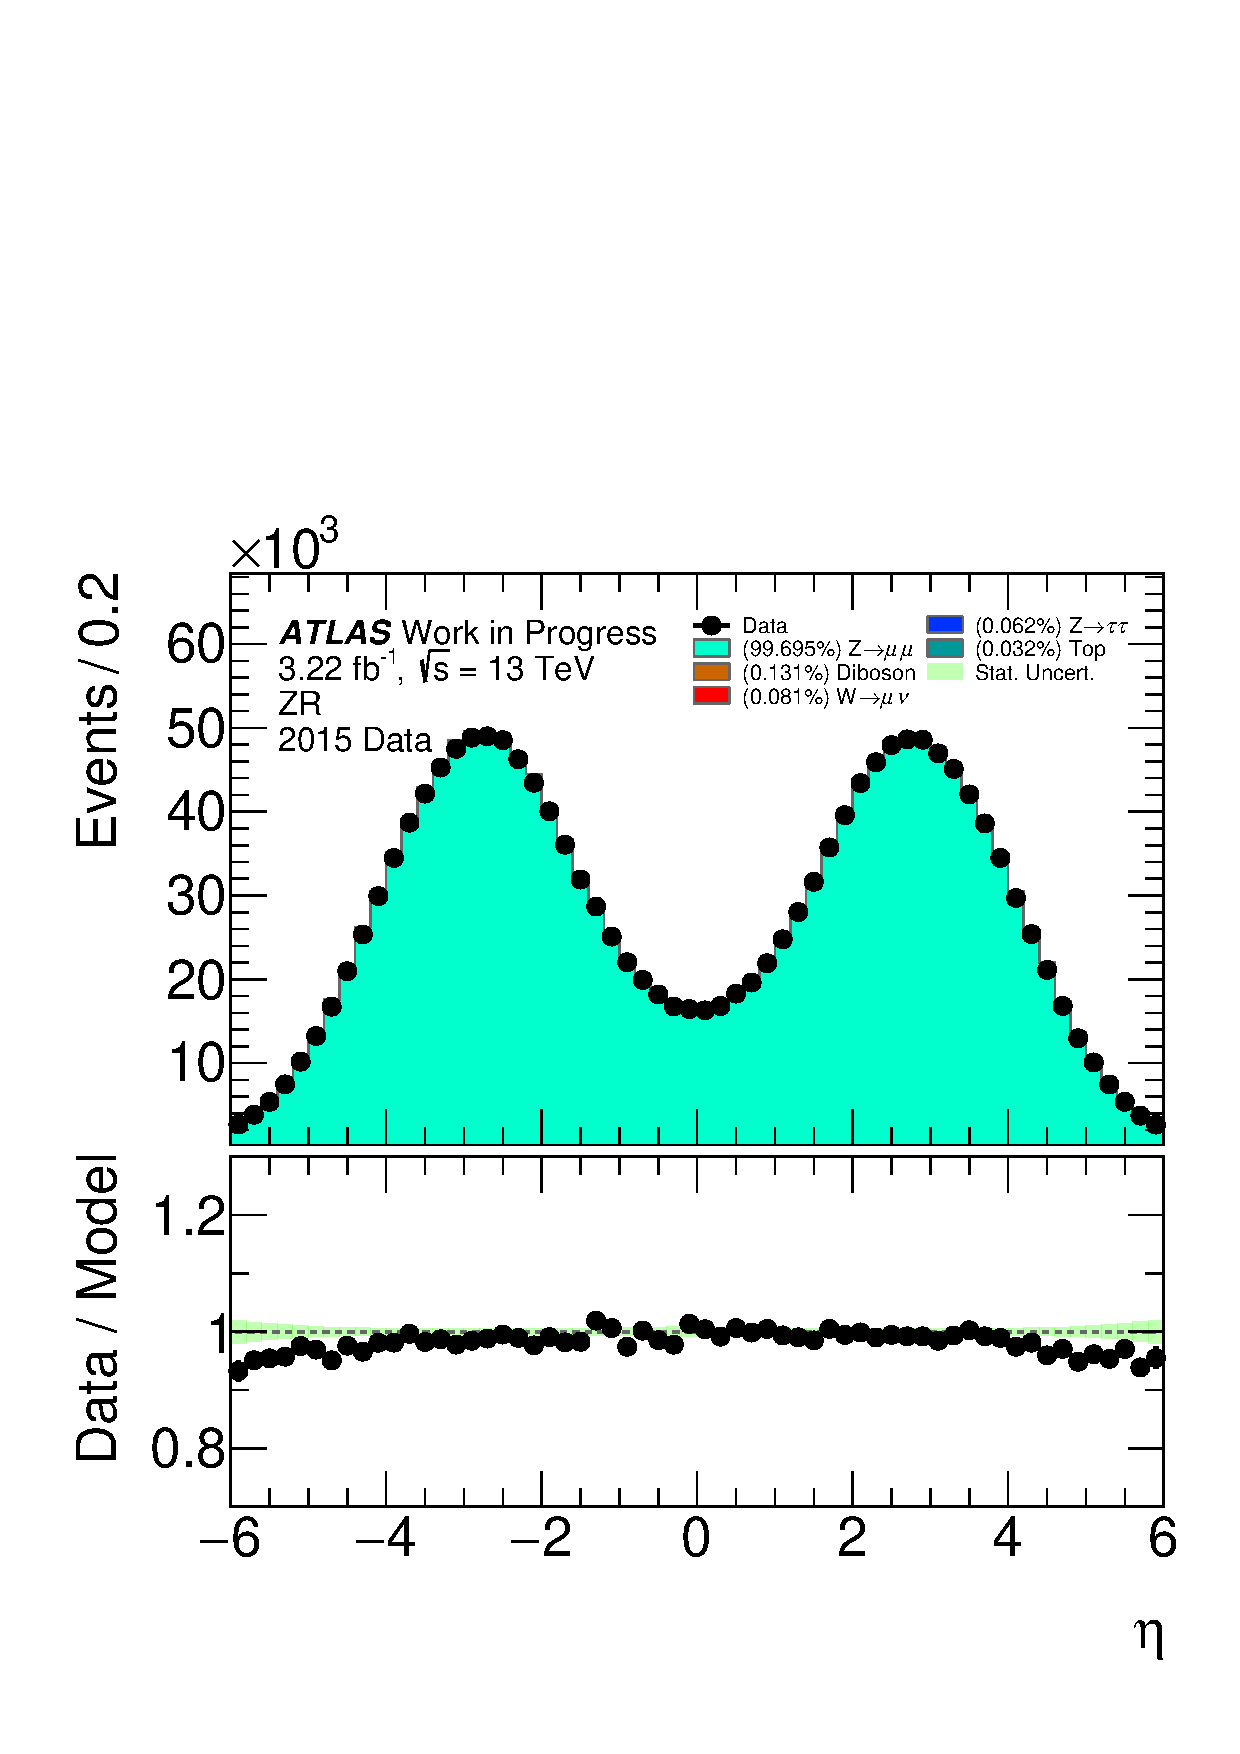
\includegraphics[width=0.45\textwidth]{figures/ZR/dataMc-dilep_eta-ZR-mu.pdf}
\caption{
Z boson pseudorapidity distribution after the $Z \rightarrow e^+e^-$ selection (left) and the $Z \rightarrow \mu^+\mu^-$  selection (right).
The expected contributions from all backgrounds are estimated with Monte Carlo simulations.
The background processes are heavily suppressed and not visible on the linear scale. 
% Systematic uncertainties for the signal and background distributions are combined in the shaded band, and 
Statistical uncertainties are shown on the data points.
Luminosity uncertainties are not included.
}
\label{fig:ZR_dilep_eta}
\end{figure}

\subsection{Background-subtracted W and Z candidate events}
\label{sec:Background_subtracted_candidate_events}

Tables~\ref{tbl:SR_observed_candidates} and~\ref{tbl:ZR_observed_candidates} summarise the numbers of observed candidate events for the $W \rightarrow \ell\nu$ and $Z \rightarrow \ell\ell$ channels, respectively, and include the number of expected background events from both the multijet process and electroweak plus $t\bar{t}$ processes and the number of background-subtracted signal events. 
The first uncertainty is due to statistics. 
% Monte Carlo statistical uncertainties are considered to be negligible in comparison to the statistical uncertainties associated to the data and to the estimation of the QCD background. 
\todo{The second uncertainty is a systematic one.}
The QCD background systematic uncertainties were explained in Section~\ref{sec:bkg_mj}. 
\todo{The luminosity determination uncertainty of 5\% is used.}

% ################################
% SR background composition table
% ################################

% \begin{table}[h]
% \begin{center}
%  \begin{tabular}{ | c || c || c | c || c |  } 
%  \hline
%  $\ell$ & Observed   &  Background & Background & Background-subtracted \\
%         & candidates & (EW + top)  & (Multijet) & Signal $N_{W\tau}^{sig}$ \\
%  \hline
%  \hline
%  $e^{\pm}$ &    &   &  & \\
%  \hline
%  $\mu^{\pm}$ &    &   &  & \\
%  \hline
% \end{tabular}
% \caption{
% Numbers of observed candidate events for the $W \rightarrow \tau\nu \rightarrow \ell\nu\nu$ channel, electroweak (EW) plus top, and data derived QCD background events, and background-subtracted signal events. 
% The first uncertainty is statistical.
% The second uncertainty represents the systematics (as described in the text).
% In addition to what is quoted in this table, \todo{an 5\%} uncertainty on the luminosity determination is applicable to the electroweak plus top background.
% The uncertainty considered for the EW+top backgrounds is the combination of the experimental uncertainties, described in \todo{Section 6}, the \todo{NNLO normalisation uncertainties}, described in \todo{Table 9}, and the statistical uncertainty on the MC.
% The uncertainty on the multijet estimate \todo{is shown as stat+syst}, as described in Section~\ref{sec:bkg_mj}.
% On $N - B$ the data statistical uncertainty, and the total systematic ones, obtained summing in quadrature the EW+top uncertainties, and the multijet statistical and systematic uncertainties.
% }
% \label{tbl:SR_observed_candidates}
% \end{center}
% \end{table}

\begin{table}[h]
\begin{center}
\begin{tabular}{ | c || c || c | c || c |  }
\hline
$\ell$ & Observed   &  Background & Background & Background-subtracted \\
        & candidates & (EW + top)  & (Multijet) & Signal $N_{W\tau}^{sig}$ \\
\hline
\hline
$e^{\pm}$ & 15844096.00 $\pm$ 3980.46 & 14448983.00 $\pm$ 11936.92 & 0.00 $\pm$ 0.00 & 1395113.00 $\pm$ 12583.09\\
\hline
$\mu^{\pm}$ & 16667946.00 $\pm$ 4082.64 & 16223126.65 $\pm$ 13865.15 & 0.00 $\pm$ 0.00 & 444819.35 $\pm$ 14453.73\\
\hline
\end{tabular}
\caption{
Numbers of observed candidate events for the $W \rightarrow \tau\nu \rightarrow \ell\nu\nu$ channel, electroweak (EW) plus top, and data derived QCD background events, and background-subtracted signal events.
The first uncertainty is statistical.
The second uncertainty represents the systematics (as described in the text).
% In addition to what is quoted in this table, \todo{an 5\%} uncertainty on the luminosity determination is applicable to the electroweak plus top background.
% The uncertainty considered for the EW+top backgrounds is the combination of the experimental uncertainties, described in \todo{Section 6}, the \todo{NNLO normalisation uncertainties}, described in \todo{Table 9}, and the statistical uncertainty on the MC.
The uncertainty on the multijet estimate \todo{is shown as stat+syst}, as described in Section~\ref{sec:bkg_mj}.
On $N - B$ the data statistical uncertainty, and the total systematic ones, obtained summing in quadrature the EW+top uncertainties, and the multijet statistical and systematic uncertainties.
}
\label{tbl:SR_observed_candidates}
\end{center}
\end{table}

% ################################
% ZR background composition table
% ################################

\begin{table}[h]
\begin{center}
\begin{tabular}{ | c || c || c || c |  }
\hline
$\ell$ & Observed   &  Background & Background-subtracted \\
        & candidates & (EW + top)  & Signal $N_{Z}^{sig}$ \\
\hline
\hline
$e^{\pm}$ & 1456927.00 $\pm$ 1207.03 & 4603.41 $\pm$ 120.20 & 1452323.59 $\pm$ 1213.00\\
\hline
$\mu^{\pm}$ & 1676489.00 $\pm$ 1294.79 & 5151.34 $\pm$ 139.06 & 1671337.66 $\pm$ 1302.24\\
\hline
\end{tabular}
\caption{
Numbers of observed candidate events for the $Z \rightarrow \ell\ell$ channel, electroweak (EW) plus top, and multijet background events, and background-subtracted signal events.
The first uncertainty is statistical.
The second uncertainty represents the systematics (as described in the text).
% In addition to what is quoted in this table, \todo{an 5\%} uncertainty on the luminosity determination is applicable to the electroweak plus top background.
The multijet background is estimated to have less than 0.1\% contribution and neglected.
}
\label{tbl:ZR_observed_candidates}
\end{center}
\end{table}

\clearpage

% %-------------------------------------------------------------------------------
% \section{The definition of $d_0$ and its optimisation}
% \label{sec:d0optimisation}
% %-------------------------------------------------------------------------------
% 
In this analysis we use a definition of d0 that is relative to the beam line, and additionally correct for some global biases due to mis-alignment in the data only based on the year and period that the data is taken.
% These choices are explained in this section.

% \subsection{Beam Line} % vs Primary Vertex Reference Frame
% \label{sec:d0_beamLineVsprimaryVertex}

% By default in the ATLAS software d0 is defined with respect to the beam line. This gives a global reference frame for which it can be defined for any vertex, and for events without any primary vertex. 
% In this analysis we keep this reference frame such that muons in our control selection of $Z \rightarrow \mu\mu$ events have identical resolution to those in our signal $W$ selection. 
% In this section we briefly discuss this choice and alternatives.

\subsection{Alignment Corrections}
\label{sec:corrections}

% \begin{figure}[htbp]
% \centering
% \subfloat[Data 2017]{{\includegraphics[width=0.45\textwidth]{figures/intro/rdrds_summer18.png} }}
% \subfloat[Data 2018]{{\includegraphics[width=0.45\textwidth]{figures/intro/rdrds_summer18.png} }}
% \caption{
%   The $d_0$ distribution for probe muons in 2017 (blue) and 2018 (red) data in the $Z$ control selection. 
%   Gaussian fits are performed to determine any global mis-alignment and the resolution. 
%   Good alignment is seen in both datasets with sub-micro offsets from zero and there is reasonable agreement between the years in the resolution. 
%   This shows that the lack of re-processing of the 2018 data does not cause significant issues for this analysis.
% }
% \label{fig:d0_2017_2018}
% \end{figure}

% The inner detector tracking group ensures that the detector is properly aligned in the data. 
% The 2018 data has not been reprocessed as the alignment was deemed good enough for analyses based on the 2017 conditions. 
% Figure \ref{fig:d0_2017_2018} shows that the 2017 and 2018 data appear to have sub-micron offsets in $d_0$ such that any correction to re-center these distributions would not significantly improve the resolution. 
% Additionally the resolution of $d_0$ is very similar between the years indicating that the lack of re-processing of 2018 data is not a large issue for this analysis.

% After re-processing of the data there can remain residual imperfections in the alignment. 
% These can results in charge dependent or charge independent biases in the $d_0$ distribution. 
The time dependent, charge independent, bias of the $d_0$ distribution is shown in Fig.\ref{fig:d0_bias_per_years}. 
Clearly in 2015 
% and 2016 
there remains a significant bias.
% , while in 2017 and 2018 data the biases are small. 
Therefore in the analysis we correct $d_0$ using a simple charge independent shift in the $d_0$ value:
\begin{equation}
  \label{eq:d0bias}
  d_0^{'} = d_0 - \alpha
\end{equation}
for 2015 data where $\alpha = -0.004479 \pm 0.000013$ mm.
% , 2016 data in periods A+B (\todo{$\alpha = XX(\pm XX)$} mm), and the remainder of 2016 data (\todo{$\alpha = XX(\pm XX)$} mm).
We additionally check that these corrections are appropriate for all $p_T$, $\eta$, and $\varphi$ in \ref{fig:d0_bias_eat_pt} and see that the same correction can be applied independent of momentum and position.

These corrections to the 2015 data 
% and 2016 
are in agreement with corrections obtained by the Top group in the $t\bar{t}$ analysis \cite{Mcfayden:2667199} and are applied in the remainder of this analysis.

\begin{figure}[htbp]
\centering
\subfloat[2015 Data]{{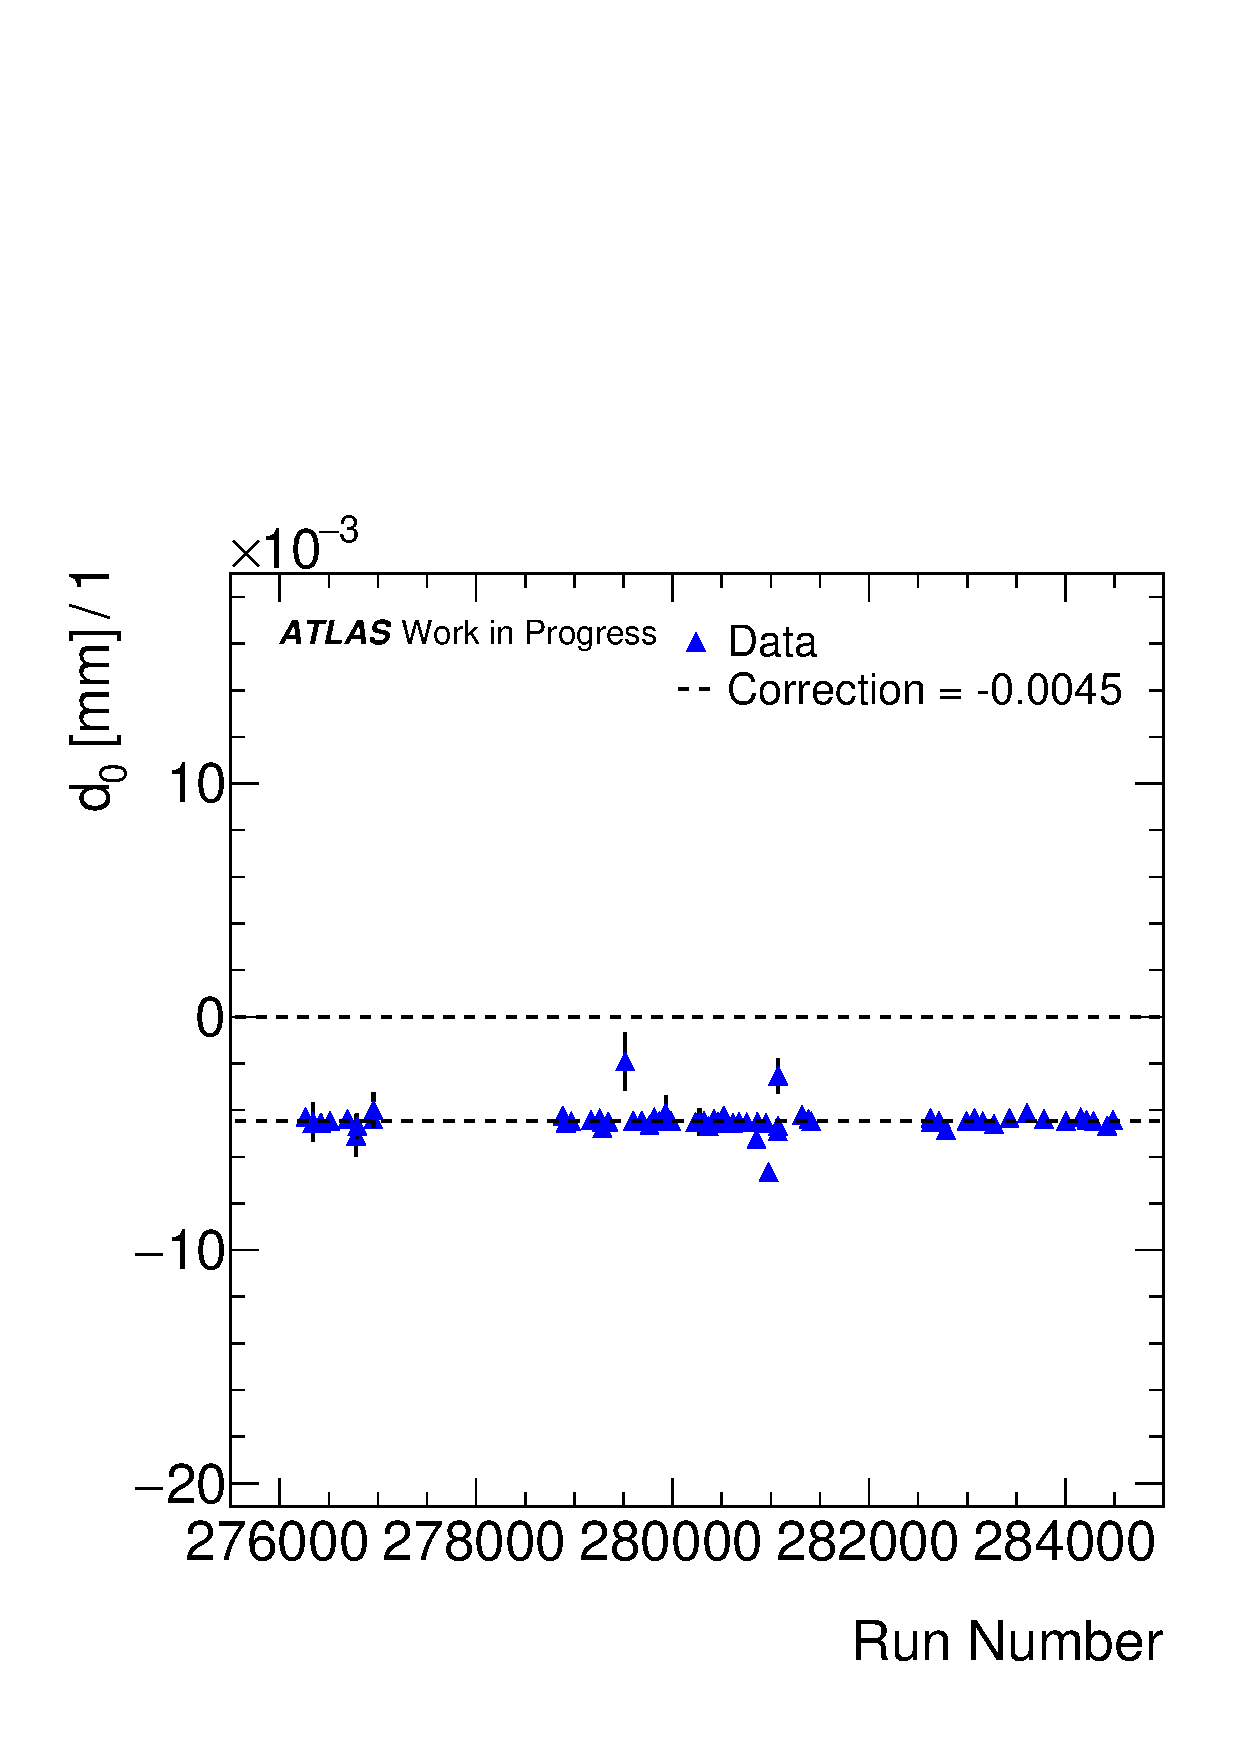
\includegraphics[width=0.45\textwidth]{figures/d0_bias/profile_lep_0_trk_d0_vs_RunNumber15-ZR-mu.pdf} }}
% \subfloat[2016 Data]{{\includegraphics[width=0.45\textwidth]{figures/intro/rdrds_summer18.png} }}
% \\
% \subfloat[2017 Data]{{\includegraphics[width=0.45\textwidth]{figures/intro/rdrds_summer18.png} }}
% \subfloat[2018 Data]{{\includegraphics[width=0.45\textwidth]{figures/intro/rdrds_summer18.png} }}
\caption{
  The average $d_0$ of leading leptons in $Z \rightarrow \mu\mu$ selection across 2015 year
%   different years 
  by RunNumber.
  The 
%   biases in 2017 and 2018 are very small but 
  significant biases relative to the resolution are seen in 2015 
%   and 2016 
  which we correct for.
}
\label{fig:d0_bias_per_years}
\end{figure}


\begin{figure}[htbp]
\centering
\subfloat[$\eta$ 2015]{{\includegraphics[width=0.31\textwidth]{figures/d0_bias/profile_lep_0_trk_d0_vs_lep_0_eta-ZR-mu.pdf} }}
\subfloat[$\varphi$ 2015]{{\includegraphics[width=0.31\textwidth]{figures/d0_bias/profile_lep_0_trk_d0_vs_lep_0_phi-ZR-mu.pdf} }}
\subfloat[$p_T$ 2015]{{\includegraphics[width=0.31\textwidth]{figures/d0_bias/profile_lep_0_trk_d0_vs_lep_0_pt-ZR-mu.pdf} }}
% \\
% \subfloat[$\eta$ 2016AB]{{\includegraphics[width=0.31\textwidth]{figures/intro/rdrds_summer18.png} }}
% \subfloat[$\varphi$ 2016AB]{{\includegraphics[width=0.31\textwidth]{figures/intro/rdrds_summer18.png} }}
% \subfloat[$p_T$ 2016AB]{{\includegraphics[width=0.31\textwidth]{figures/intro/rdrds_summer18.png} }}
% \\
% \subfloat[$\eta$ 2016Cp]{{\includegraphics[width=0.31\textwidth]{figures/intro/rdrds_summer18.png} }}
% \subfloat[$\varphi$ 2016Cp]{{\includegraphics[width=0.31\textwidth]{figures/intro/rdrds_summer18.png} }}
% \subfloat[$p_T$ 2016Cp]{{\includegraphics[width=0.31\textwidth]{figures/intro/rdrds_summer18.png} }}
% \\
% \subfloat[$\eta$ 2017]{{\includegraphics[width=0.31\textwidth]{figures/intro/rdrds_summer18.png} }}
% \subfloat[$\varphi$ 2017]{{\includegraphics[width=0.31\textwidth]{figures/intro/rdrds_summer18.png} }}
% \subfloat[$p_T$ 2017]{{\includegraphics[width=0.31\textwidth]{figures/intro/rdrds_summer18.png} }}
% \\
% \subfloat[$\eta$ 2018]{{\includegraphics[width=0.31\textwidth]{figures/intro/rdrds_summer18.png} }}
% \subfloat[$\varphi$ 2018]{{\includegraphics[width=0.31\textwidth]{figures/intro/rdrds_summer18.png} }}
% \subfloat[$p_T$ 2018]{{\includegraphics[width=0.31\textwidth]{figures/intro/rdrds_summer18.png} }}
\caption{
  The dependence on $p_T$, $\eta$, and $\varphi$ of the bias in $d_0$ of the probe lepton in $Z \rightarrow \mu\mu$ selection in 2015 year.
%   different years and periods.
}
\label{fig:d0_bias_eat_pt}
\end{figure}



\subsubsection{Calibration of impact parameter of prompt muons}
\label{sec:d0calibration_of_prompt_muons}

The calibration of $d_0$ distribution of prompt leptons is performed using $Z^{0}\rightarrow\mu^{+}\mu^{-}$ events. The selection of the calibration sample is same as described in Section~\ref{sec:z_boson_selection}.

We perform the calibration independently for each year of data taking.
The obtained samples contain mainly prompt leptons coming from $Z^{0}\rightarrow\mu^{+}\mu^{-}$ with a very small contamination from other sources.
The details on the origin of the tag lepton in the 2015 sample are shown on \ref{fig:Zmumu_mass_composition}.
The composition of the samples in other years is similar.
Hence, the impact of systematic uncertainties due to modelling of different processes on the calibration procedure is negligible.

\begin{figure}[htbp]
\centering
\includegraphics[width=0.45\textwidth]{figures/ZR/dataMc-dilep_m-ZR-mu.pdf}
\caption{
   Classification of the probe leptons in the 2015 $\mu^+\mu^-$ sample selected for $d_0$ calibration.
}
\label{fig:Zmumu_mass_composition}
\end{figure}

The $d_0$ distribution varies for different values of $p_T$ and $\eta$ of the leading lepton as demonstrated in Figures \ref{fig:d0_2015_pTDep} and \ref{fig:d0_2015_etaDep}. 
It can be seen that the dependence of d0 distribution on the lepton $p_T$ is strong.
The variation of the distributions with the change of $\eta$ is also visible.
Therefore, we determine the $d_0$ distribution separately in several kinematic bins depending on $p_T$ and $|\eta|$ of the leading lepton.

\begin{figure}[htbp]
\centering
\includegraphics[width=0.45\textwidth]{figures/ZR/d0_smearing/twoplots_TwoPlots_pT-fit_fabs_lep_0_trk_d0_cor-SR-mu.pdf}
\includegraphics[width=0.45\textwidth]{figures/ZR/d0_smearing/twoplots_TwoPlots_pT-fit_fabs_lep_0_trk_d0_cor-ZR-mu.pdf}
\caption{
  Normalised $d_0$ distributions in data of muons with $30 < p_T < 35$ GeV and $80 < p_T < 250$ GeV.
  For all distributions muons with $0 < |\eta| < 0.8$ were used.
  Signal region (left) and $Z^{0}\rightarrow\mu^{+}\mu^{-}$ region (right).
}
\label{fig:d0_2015_pTDep}
\end{figure}

\begin{figure}[htbp]
\centering
\includegraphics[width=0.45\textwidth]{figures/ZR/d0_smearing/twoplots_TwoPlots_eta-fit_fabs_lep_0_trk_d0_cor-SR-mu.pdf}
\includegraphics[width=0.45\textwidth]{figures/ZR/d0_smearing/twoplots_TwoPlots_eta-fit_fabs_lep_0_trk_d0_cor-ZR-mu.pdf}
\caption{
  Normalised $d_0$ distributions in data of muons with $0 < |\eta| < 0.8$, $0.8 < |\eta| < 1.5$ and $1.5 < |\eta| < 2.5$. 
  For all distributions muons with $30 < p_T < 35$ GeV were used.
  Signal region (left) and $Z^{0}\rightarrow\mu^{+}\mu^{-}$ region (right).
}
\label{fig:d0_2015_etaDep}
\end{figure}

The whole $p_T$ range is divided into \todo{8 bins}.
The $|\eta|$ range is divided into three bins.
The details of these divisions are given in Tables~\ref{tbl:def_kinematicBinning_pT} and \ref{tbl:def_kinematicBinning_eta}.
By definition, the kinematic bin $i$ $j$ contains all muons with $p_T$ in bin $i$ and $|\eta|$ in bin $j$.
Thus, we define \todo{24} kinematic bins in total.
A considerable number of events in the selected calibration samples ensures that appropriate statistics is available in each bin.

\begin{table}[h]
\begin{center}
 \begin{tabular}{ c | c | c | c } 
 \hline
 $p_T$ bin number ($n_{p_T}$) & $p_T$ range (GeV) & $p_T$ bin number ($n_{p_T}$) & $p_T$ range (GeV) \\
 \hline
%  [27,30,35,40,45,50,65,80,250]
 0 & 27 - 30 & 5 & 50 - 65 \\
 1 & 30 - 35 & 6 & 65 - 80 \\
 2 & 35 - 40 & 7 & 80 - 250\\
 3 & 40 - 45 & & \\ % > 250??
 4 & 45 - 50 & & \\
 \hline
\end{tabular}
\caption{
    Definition of $p_T$ bins.
}%
\label{tbl:def_kinematicBinning_pT}
\end{center}
\end{table}

\begin{table}[h]
\begin{center}
 \begin{tabular}{ c | c  } 
 \hline
 $\eta$ bin number ($n_{\eta}$) & $\eta$ range \\
 \hline
%  [0, 0.8, 1.5, 2.5]
0 & 0 - 0.8 \\
1 & 0.8 - 1.5 \\
2 & 1.5 - 2.5 \\
 \hline
\end{tabular}
\caption{
    Definition of $\eta$ bins.
}%
\label{tbl:def_kinematicBinning_eta}
\end{center}
\end{table}

% To determine the impact of the difference in the $d_0$ resolution between data and MC on the $d_0$ distribution of $W \rightarrow \ell$, where $\ell = e, \mu$.
The resolution is determined by the fit to the $d_0$ distribution of muons in a sample selected in leptonic Z region. 
This sample contains mainly prompt leptons as demonstrated in Fig.\ref{fig:Zmumu_mass_composition}.
The fit is performed in each kinematic bin in the $d_0$ range between $\pm2\dot\sigma$.
% \todo{between $-0.02$ and $0.02$ mm}. 
We use a Gaussian with mean floating around zero as a fitting function.
An example of the fit for muons with $30 < p_T < 35$ GeV and $|\eta| < 0.8$ is shown in Fig.~\ref{fig:d0_2015_fitexample}.
The distribution of the $d_0$ resolution includes also the non-Gaussian tails.
% However, the Gaussian part contains significant fraction of all leptons.
% Moreover, the corrections to the $d_0$ templates due to the differences between data and MC are found to be at the level of ∼ 1\%, as shown in Fig. 23. 
Hence, using just a Gaussian part of the $d_0$ resolution is sufficient for this study.

\begin{figure}[htbp]
\centering
\includegraphics[width=0.55\textwidth]{figures/ZR/d0_smearing/fitDebug_lep_0_trk_d0_cor_kineticBinsResoFit-ZR_etaKinematicBinning_from_0p0_to_0p8_ptKinematicBinning_from_30p0_to_35p0_bin1-mu-Data.pdf}
\caption{
  The $d_0$ distribution of probe muons with $30 < p_T < 35$ GeV and $|\eta| < 0.8$ in the 2015 sample. 
  The full curve shows the fit of this distribution in the range $\pm2\dot\sigma$ by a Gaussian function. 
  The dashed curve shows the extrapolation of this curve beyond the fit range.
}
\label{fig:d0_2015_fitexample}
\end{figure}

The $d_0$ resolution of muons contained in different kinematic bins is shown in Fig.~\ref{fig:d0_resolution}.
In this figure, the kinematic bin number ($n_k$) for the kinematic bin $ij$ is defined as \todo{$n_k = i + 8\dot j$}.
The resolution in Monte Carlo is better than in data.
This effect is increased in the bins with high $p_T$ of the leading lepton.
% We also notice that the resolution is worse in 2015-2016 and is the best in the 2018 sample.

\begin{figure}[htbp]
\centering
\includegraphics[width=0.65\textwidth]{figures/ZR/d0_smearing/kinematic_lep_0_trk_d0_kineticBinsResoFit-ZR-mu.pdf} %2015
% \\
% \includegraphics[width=0.65\textwidth]{figures/intro/rdrds_summer18.png} %2016
% \\
% \includegraphics[width=0.65\textwidth]{figures/intro/rdrds_summer18.png} %2017
% \\
% \includegraphics[width=0.65\textwidth]{figures/intro/rdrds_summer18.png} %2018
\caption{
  The muon $d_0$ resolution for different kinematic bins. 
  The kinematic bin number ($n_k$) for the kinematic bin $ij$ is defined as \todo{$n_k = i + 8\dot j$}.
}
\label{fig:d0_resolution}
\end{figure}

The difference in $d_0$ resolution between data and MC must be taken into account in the $d_0$ templates for $W \rightarrow \ell$, where $\ell = e, \mu$.
We obtain the corrected $d_0$ distributions, $F^{ell}_{ij}(d_0)$, in each kinematic bin $ij$ using the following procedure.
In each MC event, on per event basis we smear the value of $d_0$ of the leptons by a Gaussian defined as:
\begin{equation}
  \label{eq:d0_smearing}
  F^{\ell}(d_{0}) = \sum^{7}_{i=0} \sum^{2}_{j=0} \left( \bar{d_0}_{ij}(MC) + (d_{0} - \bar{d_0}_{ij}(MC)) * \frac{\sigma_{ij}(RD)}{\sigma_{ij}(MC)} \right)
\end{equation}
where $\bar{d_0}_{ij}(MC)$ stands for mean value of $d_0$ distribution in Monte Carlo for the given kinematic bin $ij$ and the values of $\sigma_{ij}(RD)$ and $\sigma_{ij}(MC)$ are shown in Fig.~\ref{fig:d0_resolution}.

% The resulting corrections to the $F^{ell}(d_0)$ distributions due to the $d_0$ resolution is relatively small as it can be inferred from Fig.~\ref{fig:d0_correctionRatio_promt_mu}. 
% This figure shows the ratio of corrected and uncorrected $F^{\ell}(d_0)$ distribution.
% The variation for different values of $d_0$ is of the order \todo{of 15\%}.

% \begin{figure}[htbp]
% \centering
% \includegraphics[width=0.65\textwidth]{figures/intro/rdrds_summer18.png} %2015
% % \\
% % \includegraphics[width=0.65\textwidth]{figures/intro/rdrds_summer18.png} %2016
% % \\
% % \includegraphics[width=0.65\textwidth]{figures/intro/rdrds_summer18.png} %2017
% % \\
% % \includegraphics[width=0.65\textwidth]{figures/intro/rdrds_summer18.png} %2018
% \caption{
%   The ratio of corrected and uncorrected $F^{\ell}(d_0)$ distribution for \todo{$W \rightarrow \mu$}.
% }
% \label{fig:d0_correctionRatio_promt_mu}
% \end{figure}

\subsubsection{Impact parameter of muons produced in $\tau$-lepton decays}
\label{sec:d0calibration_of_tau_muons}

The distribution of d0 of muons produced in tauon decays (and denoted as $\tau \rightarrow \ell$, where $\ell = e, \mu$) is taken from Monte Carlo.
Therefore, the description of this variable in simulation must be tested.
This task is performed using the sample enriched in the $Z^{0}\rightarrow\tau^{+}\tau^{-}$ leptonic events.
To obtain this sample we require:
\begin{itemize}
\item one electron and one muon in the event;
\item the charges of the two leptons must be opposite;
\item \todo{$m(e\mu) < 85$} GeV
\item \todo{$p_{T}^{probe} > 15$} GeV
\end{itemize}

\todo{Show that we model Ztautau process well.}

\todo{Show that $d_0$ modelling in Ztautau match/not match data.}

\todo{If not match data, explain how we plan to apply corrections.}



\subsubsection{Impact parameter of fake muons}
\label{sec:d0calibration_of_fake_muons}

In this analysis we obtain fakes by fake factor method. 
The $d_0$ distribution of fake muons is taken from Data, after subtraction corrected MC events from the fake template region.






% %-------------------------------------------------------------------------------
% \section{Systematic uncertainties}
% \label{sec:Systematic}
% %-------------------------------------------------------------------------------
% 
\subsection{Pruning and smoothing of systematic variations}
\label{sec:pruning_smoothing}

% \subsection{Sources of uncertainty from data-driven corrections}
% \label{sec:WZ_noBkg}


% %-------------------------------------------------------------------------------
% \section{Fitting Procedure}
% \label{sec:fit}
% %-------------------------------------------------------------------------------
% 
\subsection{Fit setup}
\label{sec:fit_setup}

\subsection{Region definition and binning}
\label{sec:region_definition_and_binning}

\subsection{Fit validation}
\label{sec:fit_validation}

\subsubsection{Nuisance parameter pulls and constraints}
\label{sec:nuisance_parameter_pulls_and_constraints}

\subsubsection{Fit parameter covariance matrix}
\label{sec:fit_parameter_covariance_matrix}

\subsubsection{Nuisance parameter ranking (effect on POI)}
\label{sec:nuisance_parameter_ranking}


% %-------------------------------------------------------------------------------
% \section{Results}
% \label{sec:results}
% %-------------------------------------------------------------------------------
% 
\subsection{Prefit results}
\label{sec:prefit_results}

\subsubsection{Yields}
\label{sec:prefit_results_yields}

\subsubsection{Data/MC plots}
\label{sec:prefit_results_dataMC_plots}

\subsection{Post-fit results}
\label{sec:postfit_results}

\subsubsection{Measured $R(\tau/\ell)$ and uncertainty breakdown}
\label{sec:postfit_results_Measured_r_and_and_uncertainty_breakdown}

\subsubsection{Post-fit data/MC agreement}
\label{sec:postfit_results_dataMC_agreement}

\subsubsection{Analysis of fit results}
\label{sec:postfit_results_analysis_of_fit_results}


%-------------------------------------------------------------------------------
\section{Conclusion}
\label{sec:conclusion}
%-------------------------------------------------------------------------------

A measurement of $R(\tau/\ell)$ has been performed with direct leptonic W decay mode using a dataset corresponding to an integrated luminosity of \todo{XXX}fb$^{-1}$ of proton-proton collisions at $\sqrt{s} = 13$~TeV recorded by the ATLAS experiment at the LHC.

The expected precision on $R(\tau/\ell)$ is \todo{1.\%} and the best fit observed value of $R(\tau/\ell)$ is \todo{XX $\pm$ YY}. 
This surpasses the precision of the most precise previous measurement from LEP in WW production and \todo{[shows/does not show]} $W\sigma$ tension with the SM prediction.

%-------------------------------------------------------------------------------
% If you use biblatex and either biber or bibtex to process the bibliography
% just say \printbibliography here
\printbibliography
% If you want to use the traditional BibTeX you need to use the syntax below.
%\bibliographystyle{bib/bst/atlasBibStyleWithTitle}
%\bibliography{ANA-STDM-2018-50-INT1,bib/ATLAS,bib/CMS,bib/ConfNotes,bib/PubNotes}
%-------------------------------------------------------------------------------

%-------------------------------------------------------------------------------
% Print the list of contributors to the analysis
% The argument gives the fraction of the text width used for the names
%-------------------------------------------------------------------------------
\clearpage
\PrintAtlasContribute{0.30}


%-------------------------------------------------------------------------------
\clearpage
\appendix
\part*{Appendices}
\addcontentsline{toc}{part}{Appendices}
%-------------------------------------------------------------------------------

% %-------------------------------------------------------------------------------
% \section{List of MC samples}
% \label{sec:details_on_list_of_MC_samples}
% %-------------------------------------------------------------------------------
% 
The list of MC samples used in this analysis are shown.
% in Tables 24 and 25.
In all cases, MC16a was used for 2015 and 2016 sample, MC16d for 2017 sample and MC16e for 2018 sample.
For each sample we specify the p-tag used.
% The last columns states whether full (FS) or fast (AF) simulation was used.


\begin{table}[h]
\begin{center}
 \begin{tabular}{ l|rllrrr } 
 Sample &   DSID & Generator           & p-tag   &     xs [pb] &   $fe$ &   k-faktor \\
 \hline\hline
 $W\rightarrow\tau\nu$  & 361102 & PowhegPythia8EvtGen & p3729   & 11500.9     &   1       &    1.01724 \\
 $W\rightarrow\tau\nu$  & 361105 & PowhegPythia8EvtGen & p3729   &  8579.31    &   1       &    1.03579 \\
 $W\rightarrow e\nu$     & 361100 & PowhegPythia8EvtGen & p3731   & 11500.9     &   1       &    1.01724 \\
 $W\rightarrow e\nu$     & 361103 & PowhegPythia8EvtGen & p3731   &  8579.42    &   1       &    1.03577 \\
 $W\rightarrow\mu\nu$   & 361101 & PowhegPythia8EvtGen & p3731   & 11500.9     &   1       &    1.01724 \\
 $W\rightarrow\mu\nu$   & 361104 & PowhegPythia8EvtGen & p3731   &  8579.31    &   1       &    1.03576 \\
 $Z\rightarrow ee$      & 361106 & PowhegPythia8EvtGen & p3731   &  1950.53    &   1       &    1.026   \\
 $Z\rightarrow\mu\mu$   & 361107 & PowhegPythia8EvtGen & p3731   &  1950.63    &   1       &    1.02605 \\
 $Z\rightarrow\tau\tau$ & 361108 & PowhegPythia8EvtGen & p3729   &  1950.63    &   1       &    1.02605 \\
 Top                       & 410013 & PhPy8EG\_P2012       & p3729   &    35.8455  &   1       &    1.054   \\
 Top                       & 410014 & PhPy8EG\_P2012       & p3729   &    35.8244  &   1       &    1.054   \\
 Top                       & 410470 & PhPy8EG\_A14         & p3729   &   452.346   &   0.54385 &    1.13976 \\
 Top                       & 410644 & PowhegPythia8EvtGen & p3729   &     2.06146 &   1       &    1.017   \\
 Top                       & 410645 & PowhegPythia8EvtGen & p3729   &     1.28857 &   1       &    1.0167  \\
 Top                       & 410646 & PowhegPythia8EvtGen & p3729   &    35.8486  &   1       &    0.945   \\
 Diboson                   & 363356 & Sherpa\_221\_PDF30    & p3729   &     2.20355 &   0.14158 &    1       \\
 Diboson                   & 363358 & Sherpa\_221\_PDF30    & p3729   &     3.4328  &   1       &    1       \\
 Diboson                   & 363359 & Sherpa\_221\_PDF30    & p3729   &    24.708   &   1       &    1       \\
 Diboson                   & 363360 & Sherpa\_221\_PDF30    & p3729   &    24.724   &   1       &    1       \\
 Diboson                   & 363489 & Sherpa\_221\_PDF30    & p3729   &    11.42    &   1       &    1       \\
 Diboson                   & 364250 & Sherpa\_222\_PDF30    & p3729   &     1.2523  &   1       &    1       \\
 Diboson                   & 364253 & Sherpa\_222\_PDF30    & p3729   &     4.579   &   1       &    1       \\
 Diboson                   & 364254 & Sherpa\_222\_PDF30    & p3729   &    12.501   &   1       &    1       \\
 Diboson                   & 364255 & Sherpa\_222\_PDF30    & p3729   &     3.2344  &   1       &    1       \\
\hline
\end{tabular}
\caption{
 MC16a samples for 2015 and 2016
}%
\label{tbl:mc_samples_ewk}
\end{center}
\end{table}



% \begin{table}[h]
% \begin{center}
%  \begin{tabular}{ c | c  c  c } 
%  Sample & DSID & p-tag & Simulation \\
%  \hline\hline
%  & & & \\
%  \hline 
%  & & & \\
% \end{tabular}
% \caption{
%  MC samples Top
% }%
% \label{tbl:mc_samples_top}
% \end{center}
% \end{table}


\end{document}
